\subsection{Architettura delle informazioni}
La progettazione dell'interfaccia dell'applicazione è stata basata sul
modello top-down. Come primo step infatti, sono stati individuati i
dispositivi target e quale
struttura generale dare all'applicazione: layout delle schermate e menu di accesso
alle macrocategorie. In particolare si è deciso
di progettare l'applicazione principalemente per i dispositivi tablet, i
quali offrono uno schermo più grande rispetto agli smartphone e allo
stesso tempo offrono una buona mobilità. Scelta mossa anche dalla
considerazione che CookApp venga utilizzato in buona parte in
casa. Inoltre è stato deciso di progettare una parte di
funzionalità, quelle che necessitano di una maggiore mobilità,  anche
per gli smartwatch, sia per la facile trasportabilità che
offrono, sia per la loro crescita di mercato. Per quanto riguarda i
dispositivi, abbiamo deciso infine di considerare anche la possibilità
che un utente molto tecnologico possegga uno smartfridge, il quale
potrebbe comunicare gli ingredienti attualmente presenti al suo interno
al dispositivo su cui è installato CookApp. In questo modo si possono
filtrare facilmente i risultati di ricerca in base agli ingredienti
presenti nel frigo dell'utente.

Dopo aver pensato agli scopi dell'utente e ai mezzi utilizzati per
raggiungerli ci siamo concentrati sulla progettazione dell'interfaccia.
In particolare abbiamo optato per un'interfaccia semplice, chiara e ben
strutturata. Il layout è coerente in tutta l'applicazione e in nessuna
delle
sue diramazioni o funzioni presenta deviazioni dalla struttura decisa in
partenza. In aggiunta abbiamo posto molta attenzione nel mantenere una
struttura molto simile nell'interfaccia per smartwatch, in modo da
fornire familiarità all'utente anche dopo il cambio di dispositivo.

Infine dopo aver deciso la struttura generale dell'interfaccia abbiamo
progettato le funzionalità, dalle principali a quelle minori e di
supporto.

Vedremo in seguito tutta l'interfaccia
CookApp nel dettaglio.

\subsection{Design dell'interazione}

In figura \ref{blueprint} viene mostrato il blueprint dell'interazione
di CookApp. Si può notare come l'utente possa raggiungere le
funzionalità principali dell'applicazioni in bravi passi grazie ad
interfaccia semplice ed intuitiva. All'apertura dell'applicazione
l'utente si trova nella schermata ``Home page'' dalla quale può raggiungere 7
macrocategorie, le quali si diramano poi in diverse funzionalità che verranno
mostrate in seguito più nel dettaglio.\\
Si può inoltre notare dal blueprint che tutte le funzionalità della
sezione ``Lista della spesa''  sono raggruppate in un contenitore con la
denominazione ``SMARTWATCH''. Infatti quest'ultimo insieme di
funzionalità è disponibile anche nell'interfaccia per i dispositivi
smartwatch. Si assume che un utente utilizzi lo stesso account di
sistema tra i suoi dispositivi, i quali sincronizzano i loro dati
tramite il cloud condiviso.


\begin{landscape}
\label{fig:blueprint}
\begin{figure}[!h]
\centering
\fbox{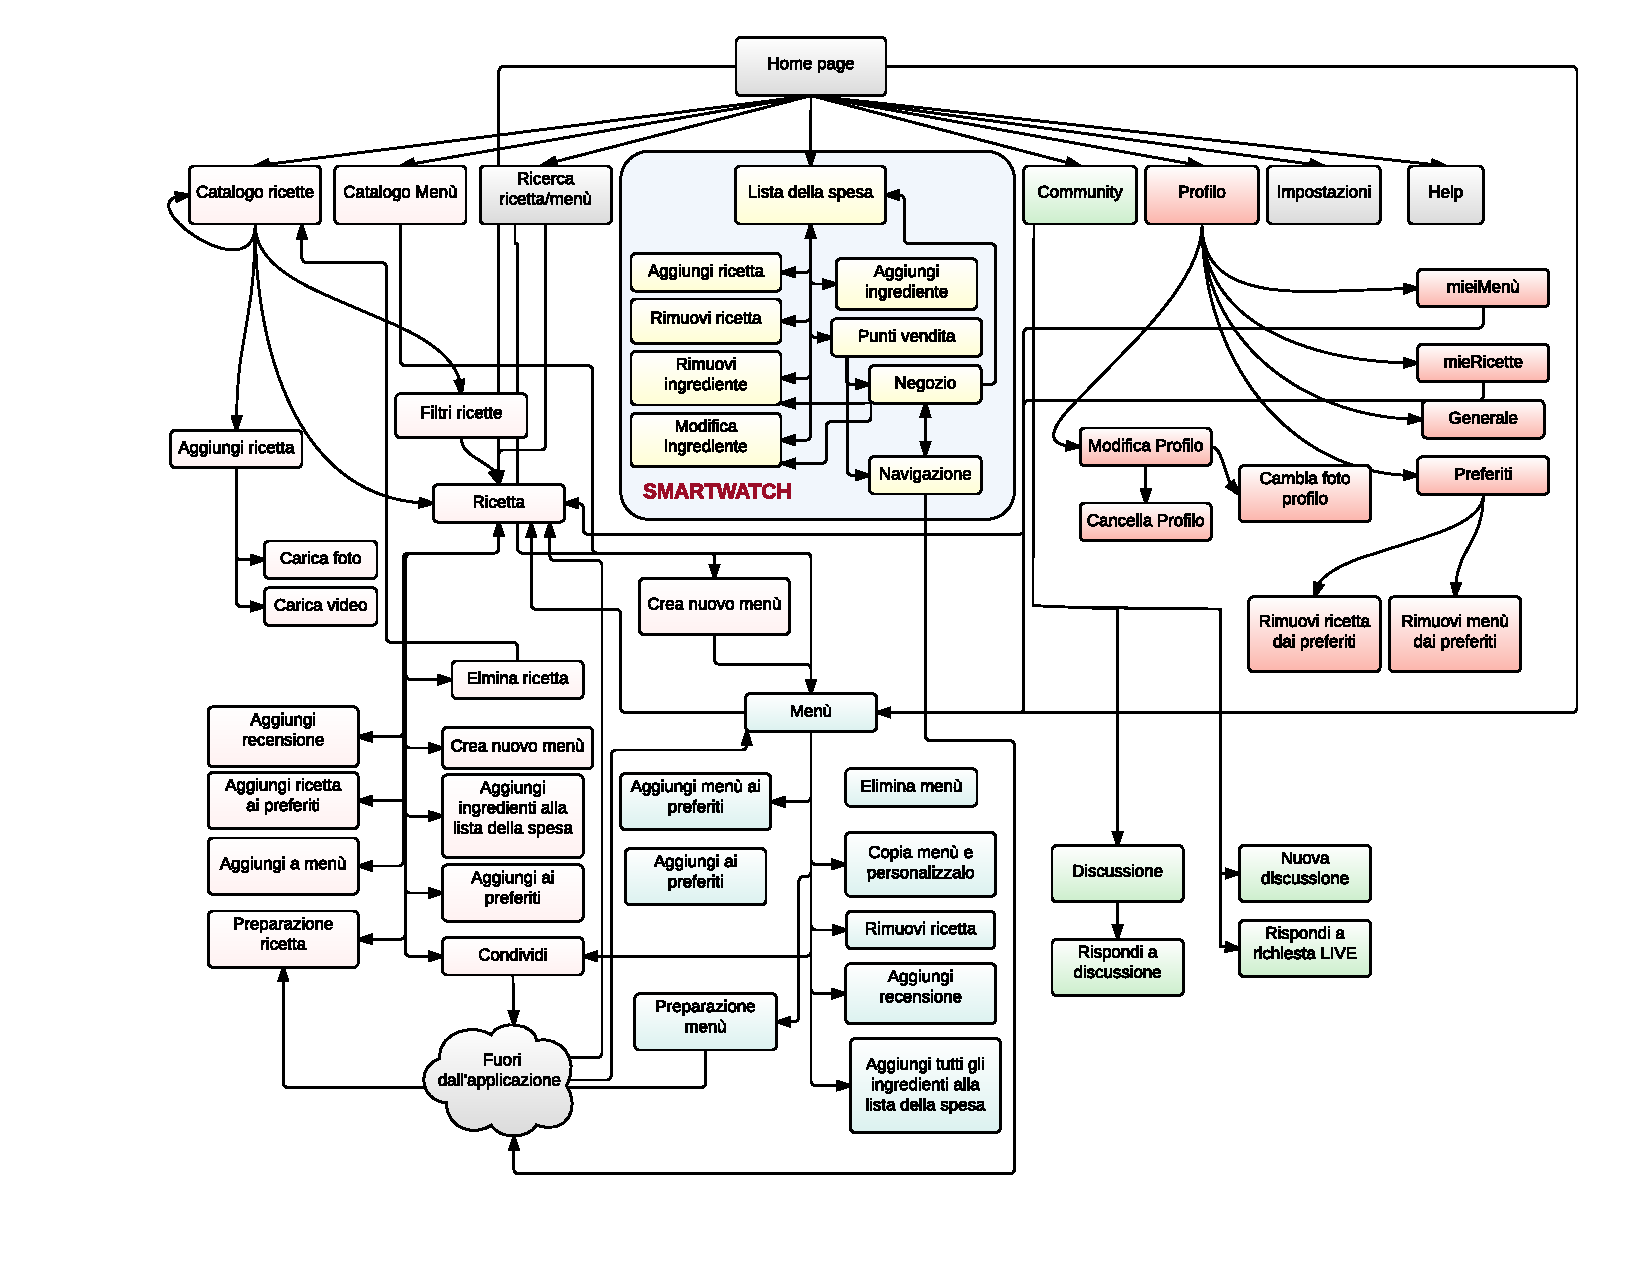
\includegraphics[width=0.9\linewidth]{img/blueprint.pdf}}
\end{figure}
\end{landscape}


\subsection{Prototipo dell'interfaccia}
\subsubsection{Homepage}
Una volta effettuato il login, all'utente viene mostrata la homepage.\\
Subito si può notare la struttura generale dell'applicazione:
\begin{itemize}
\item Una barra orizzontale posta nella parte superiore dell'app permette di fare operazioni di undo/redo per tornare in schede già visitate in precedente o per annullare certe azioni; al centro viene sempre visualizzato il logo appositamente creato mentre a destra è possibile cercare una ricetta o un menù semplicemente immettendo il nome della ricetta stessa o degli ingredienti separati da virgole; infine l'avatar a destra permette di accedere al proprio profilo.
\item La barra verticale posta a sinistra è il menù delle sezioni dell'applicazione; in ordine troviamo la homepage, il ricettario, i menù, la lista della spesa, la sezione community, le impostazioni e l'help. In fondo è visibile l'icona per i comandi vocali attivabili tramite il comando "Ehy CookAp".
\item In basso a destra è sempre visibile un'icona raffigurando la chat delle richieste di aiuto live attive. Nel momento in cui si riceve una risposta a qualche richiesta, l'icona cambia e diventa di colore giallo, in attesa di una sua lettura. Successivamente viene descritta più approfonditamente la chat.
\item Infine al centro della pagina è visibile il contenuto iniziale della homepage, in questo caso.
\end{itemize}
La homepage è il punto di ingresso dell'applicazione: al centro è possibile avere un'overview generale, un \textit{Cover flow} sfogliabile con swipe orizzontali, permette la visualizzazioni del piatto del giorno, del menù del giorno e di piatti legati a festività o eventi inerenti al periodi.\\
Sotto, invece, vi sono due scorciatoie per le ricette e i menù recentemente visitati, insieme a una serie di riquadri delle ricette più cliccate in generale.
\begin{figure}[H]
	\centering
	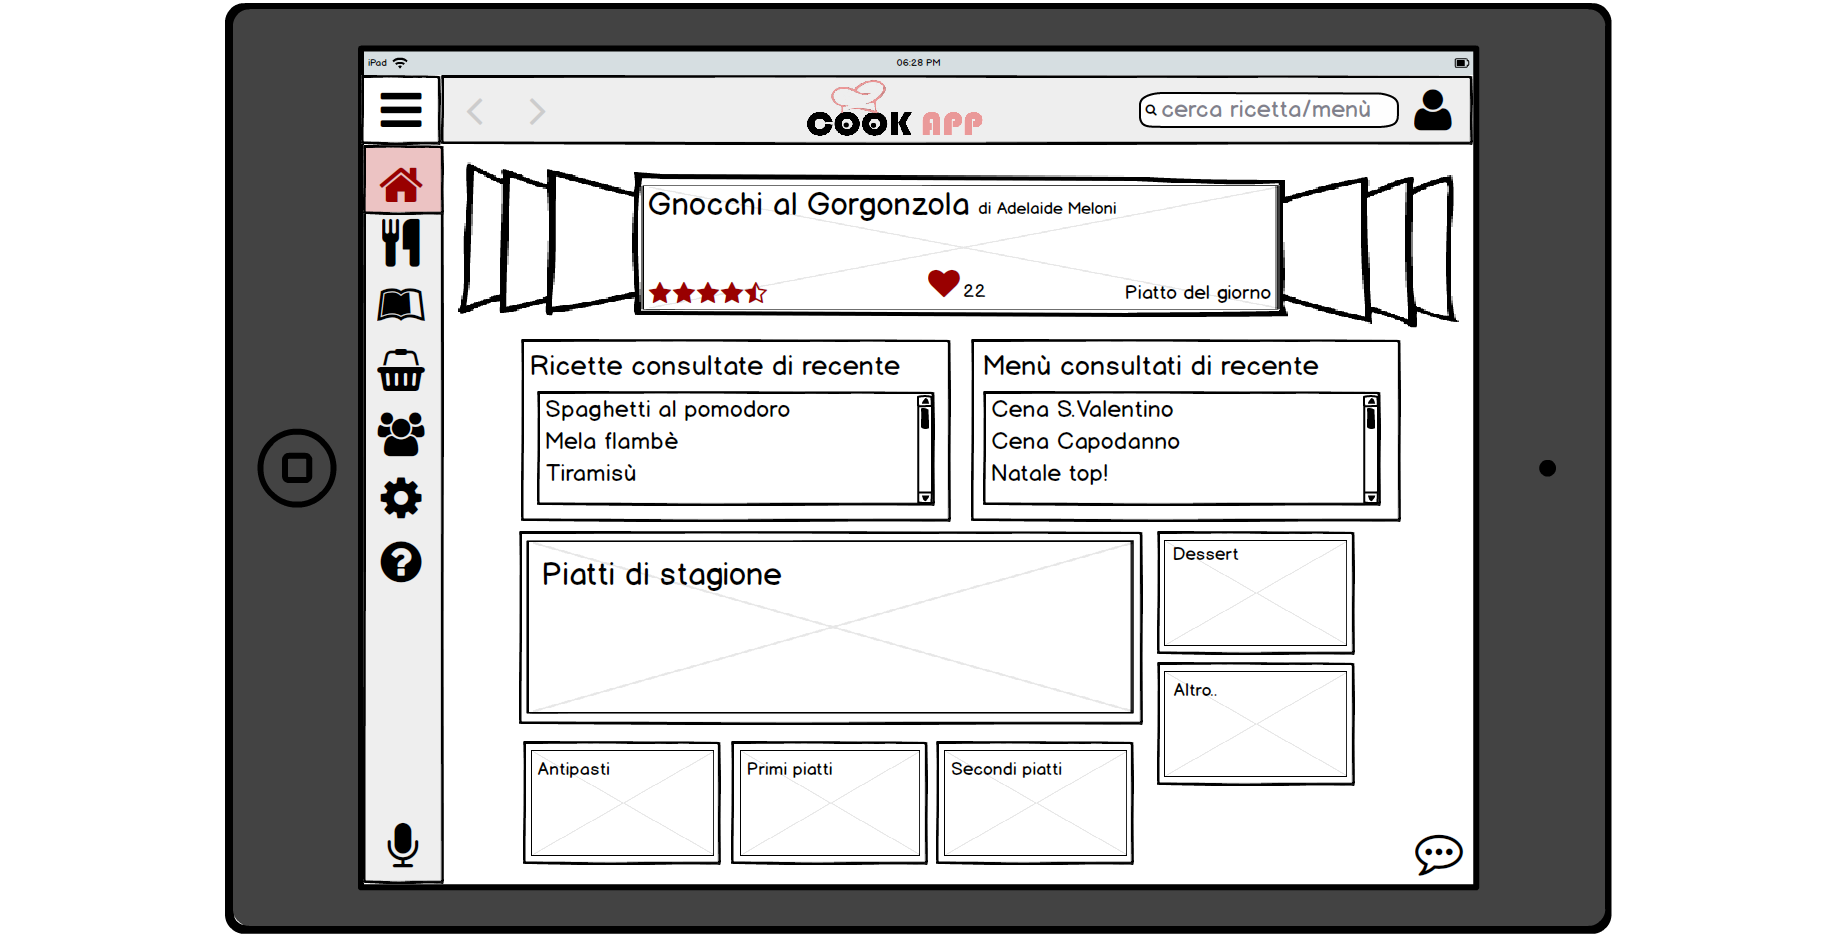
\includegraphics[width=0.95\linewidth]{img/mockup/Homepage.png}
\end{figure}
\begin{figure}[H]
	\centering
	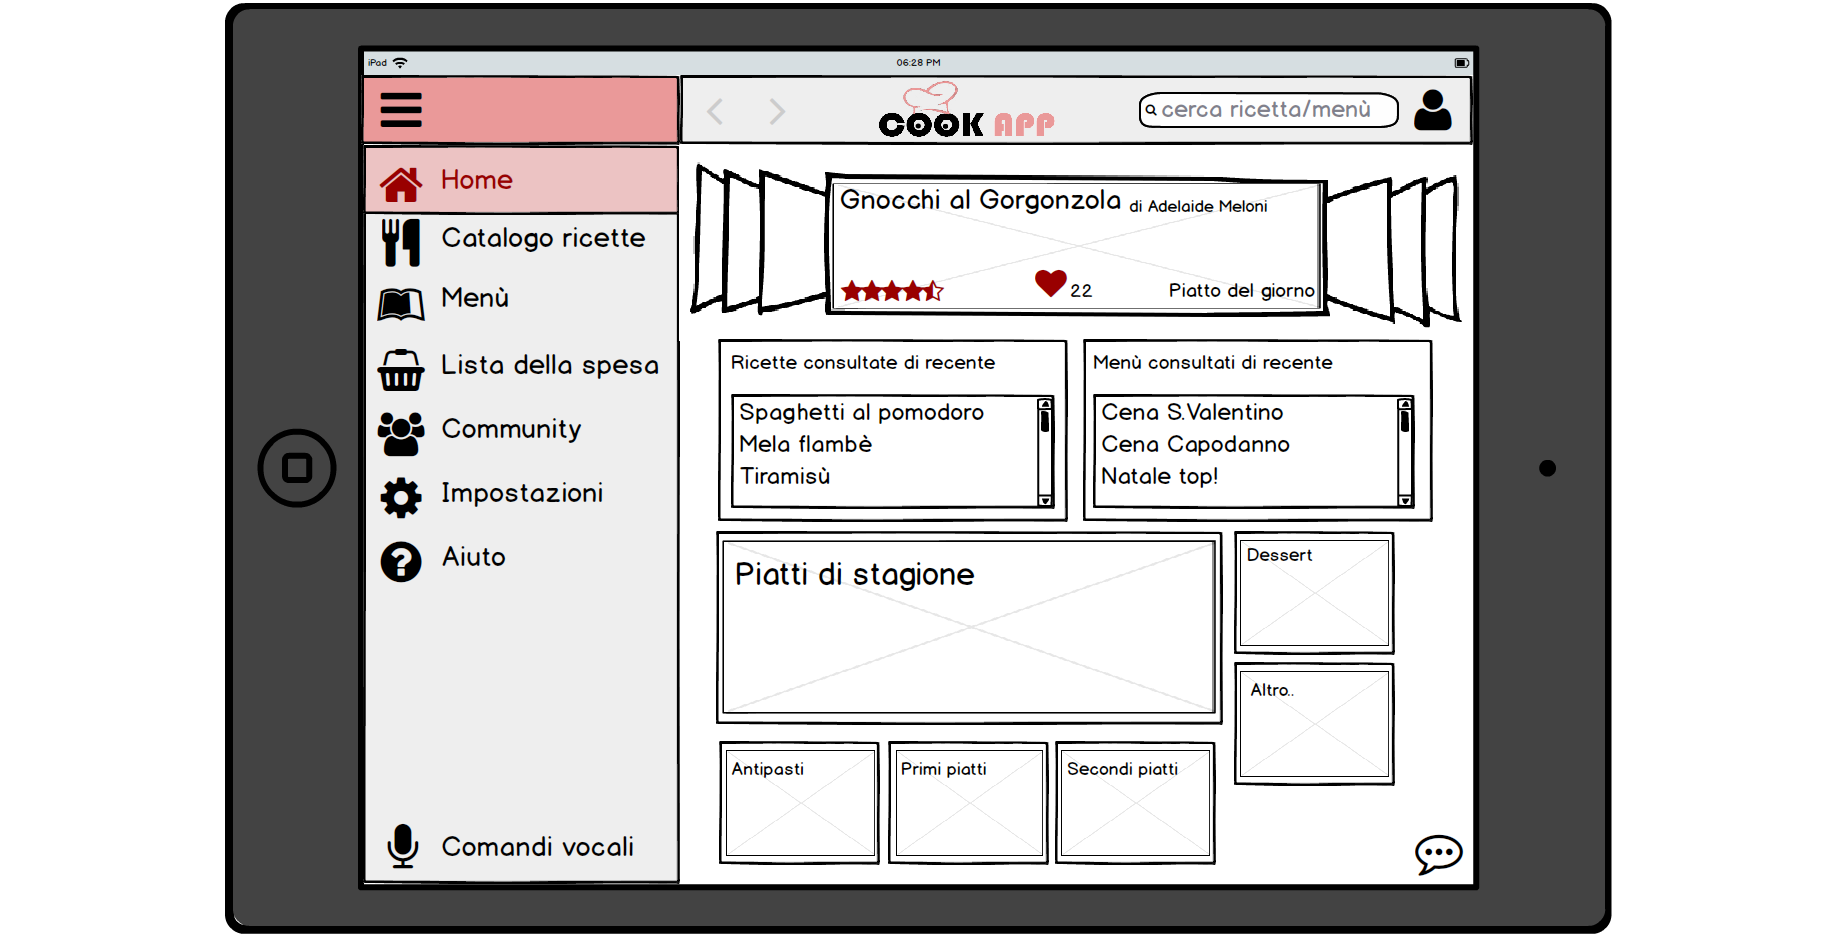
\includegraphics[width=0.95\linewidth]{img/mockup/Homepage-menu.png}
\end{figure}
\begin{figure}[H]
	\centering
	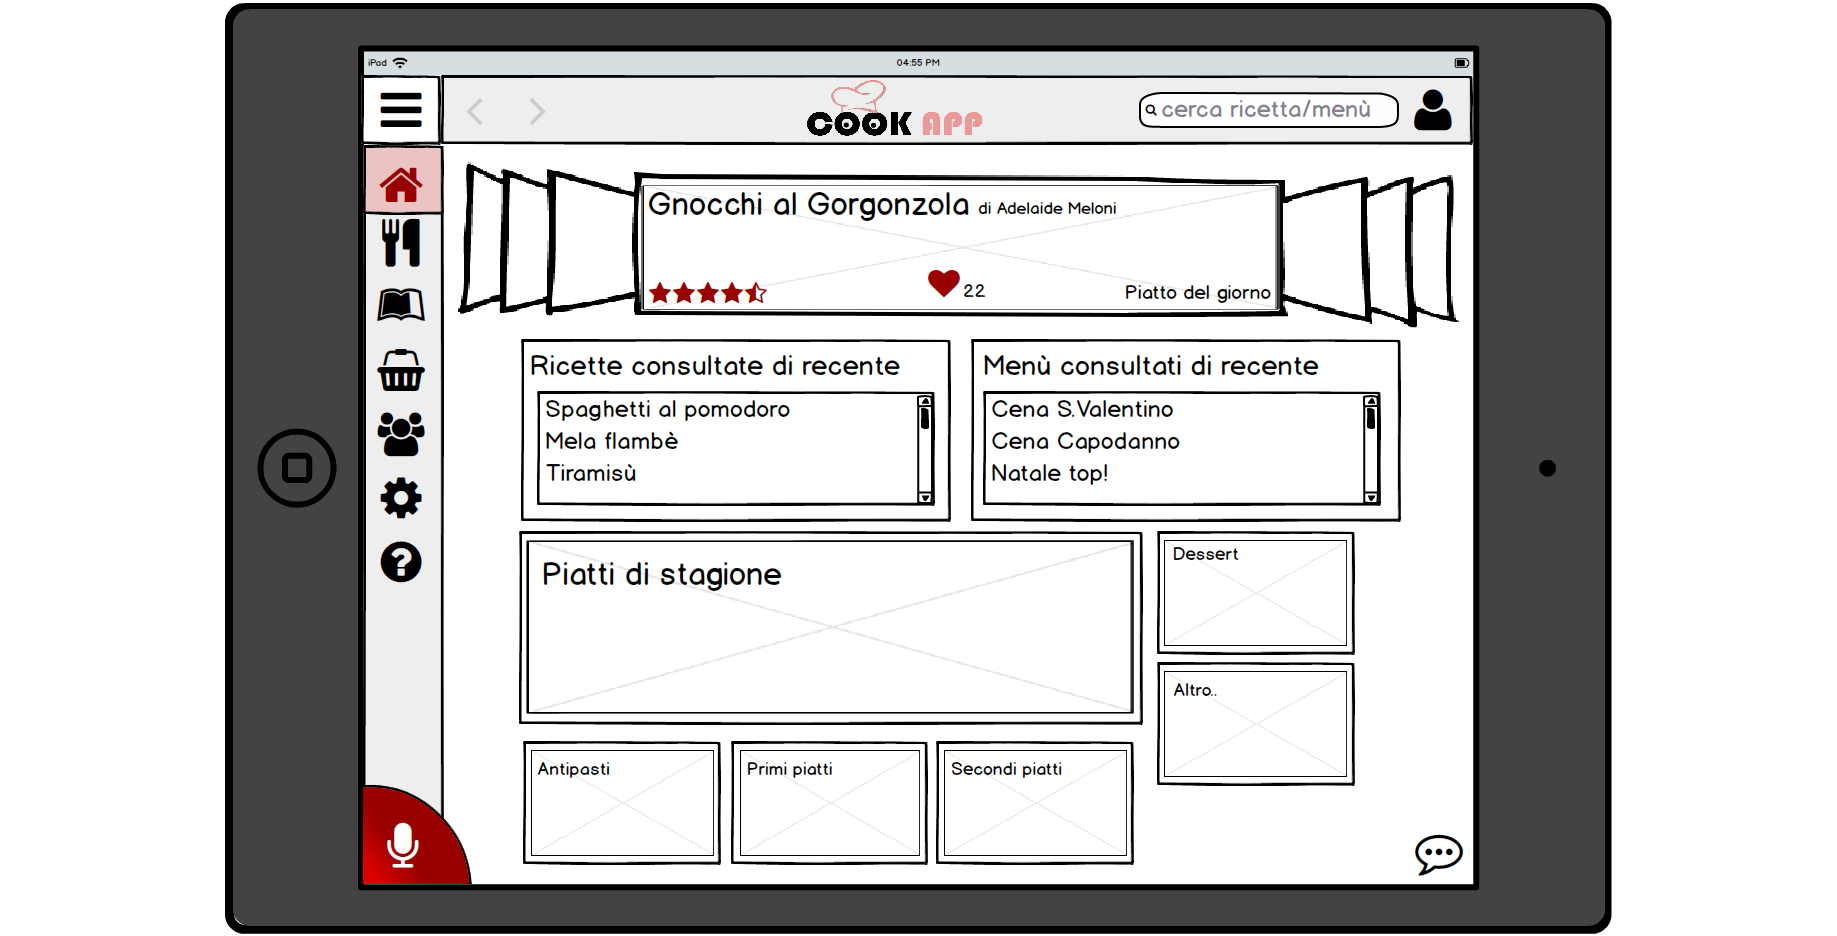
\includegraphics[width=0.95\linewidth]{img/mockup/Homepage-microphone.png}
\end{figure}

\subsubsection{Ricerca}
La barra in alto a destra permette di accedere facilmente alla
funzionalità di ricerca di ricette e menù.
\begin{figure}[H]
	\centering
	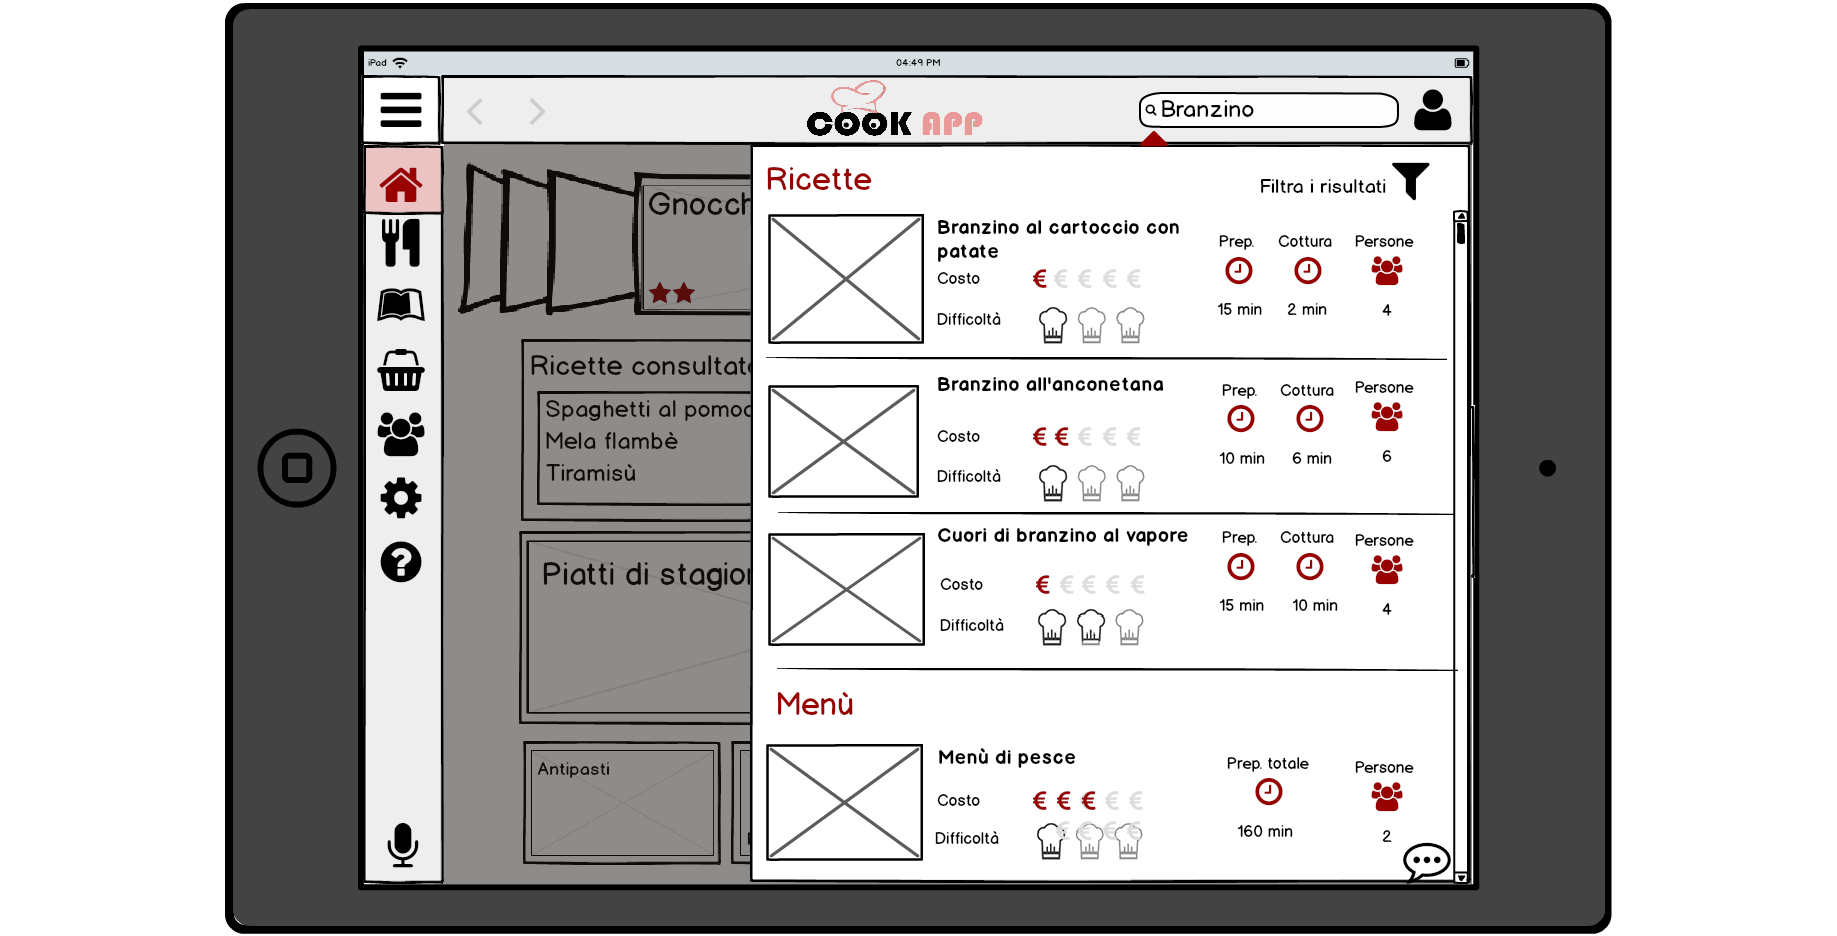
\includegraphics[width=0.95\linewidth]{img/mockup/ricerca.png}
\end{figure}


\subsubsection{Aiuto LIVE}
Ogniqualvolta un utente chieda aiuto alla community durante la preparazione di un piatto, viene automaticamente creata un'apposita voce nella sezione, sempre consultabile, degli aiuti live.\\
Ordinati in ordine cronologico, ogni voce è eliminabile in ogni momento e si presenta di diversi colori:
\begin{itemize}
\item Bianco: la richiesta è presente, ma non vi sono ancora risposte
\item Giallo: la richiesta ha alcune risposte, ma nessuna è stata selezionata come esaustiva
\item Verde: la richiesta è stata soddisfatta e non è più presente nelle richieste pendenti.
\end{itemize}
\begin{figure}[H]
	\centering
	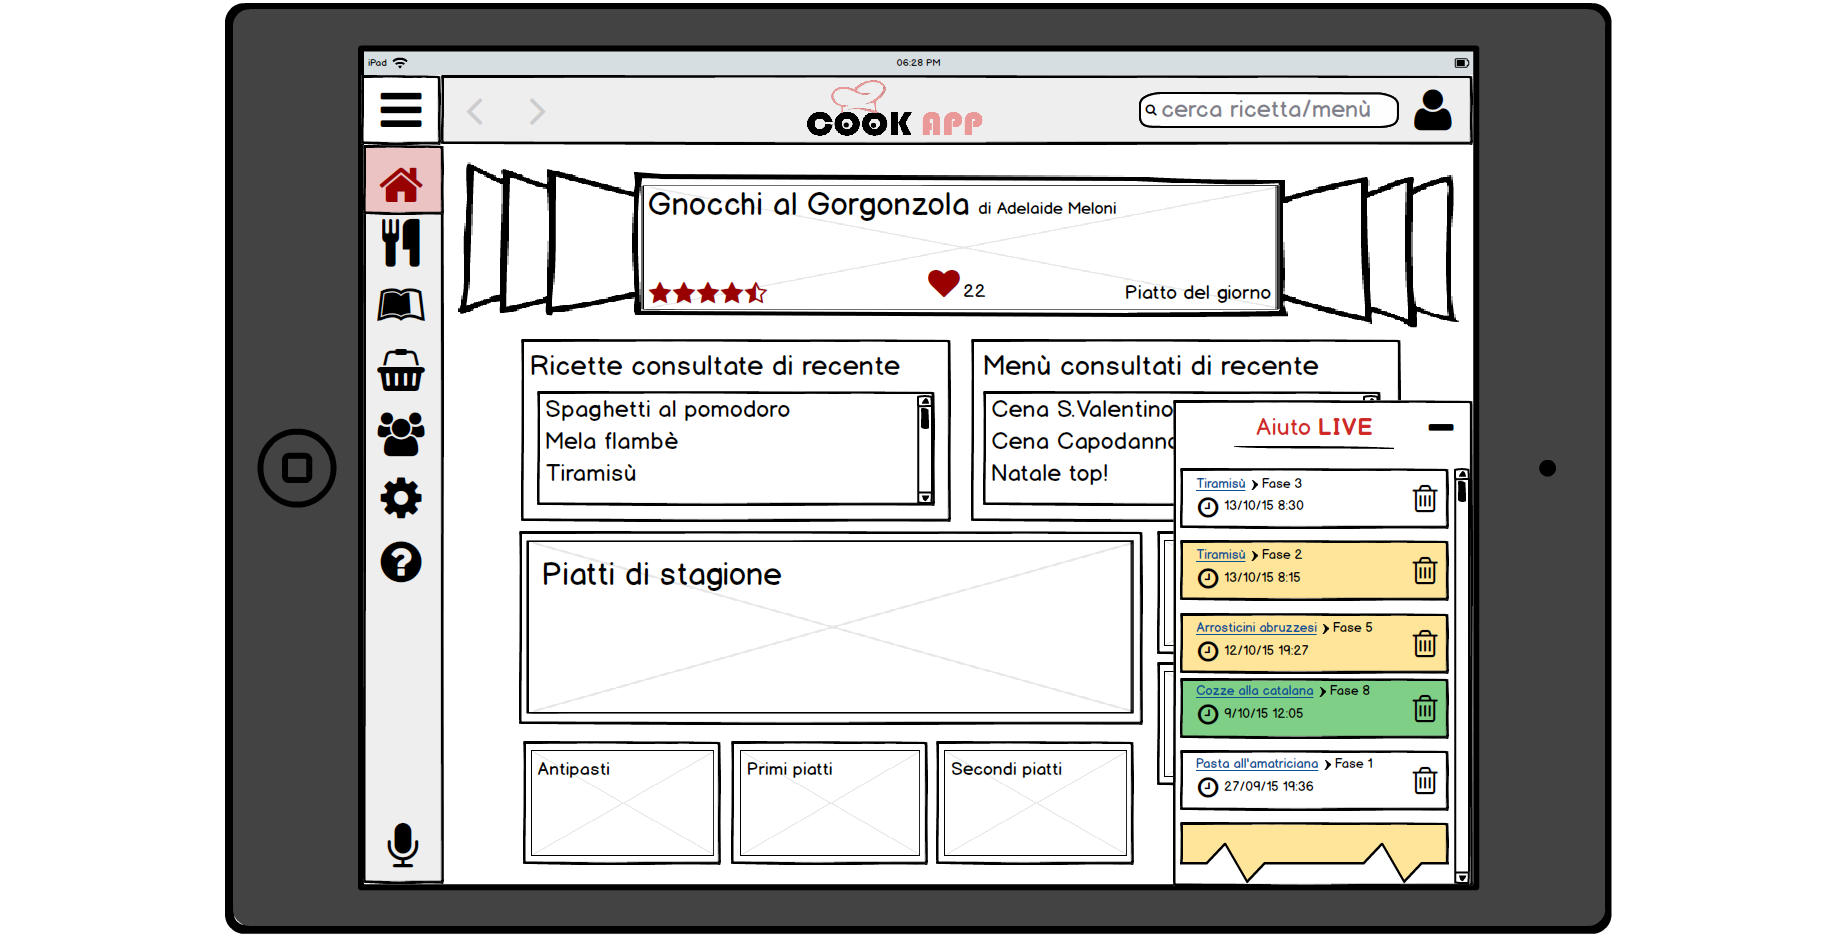
\includegraphics[width=0.95\linewidth]{img/mockup/Live1.png}
\end{figure}
\begin{figure}[H]
	\centering
	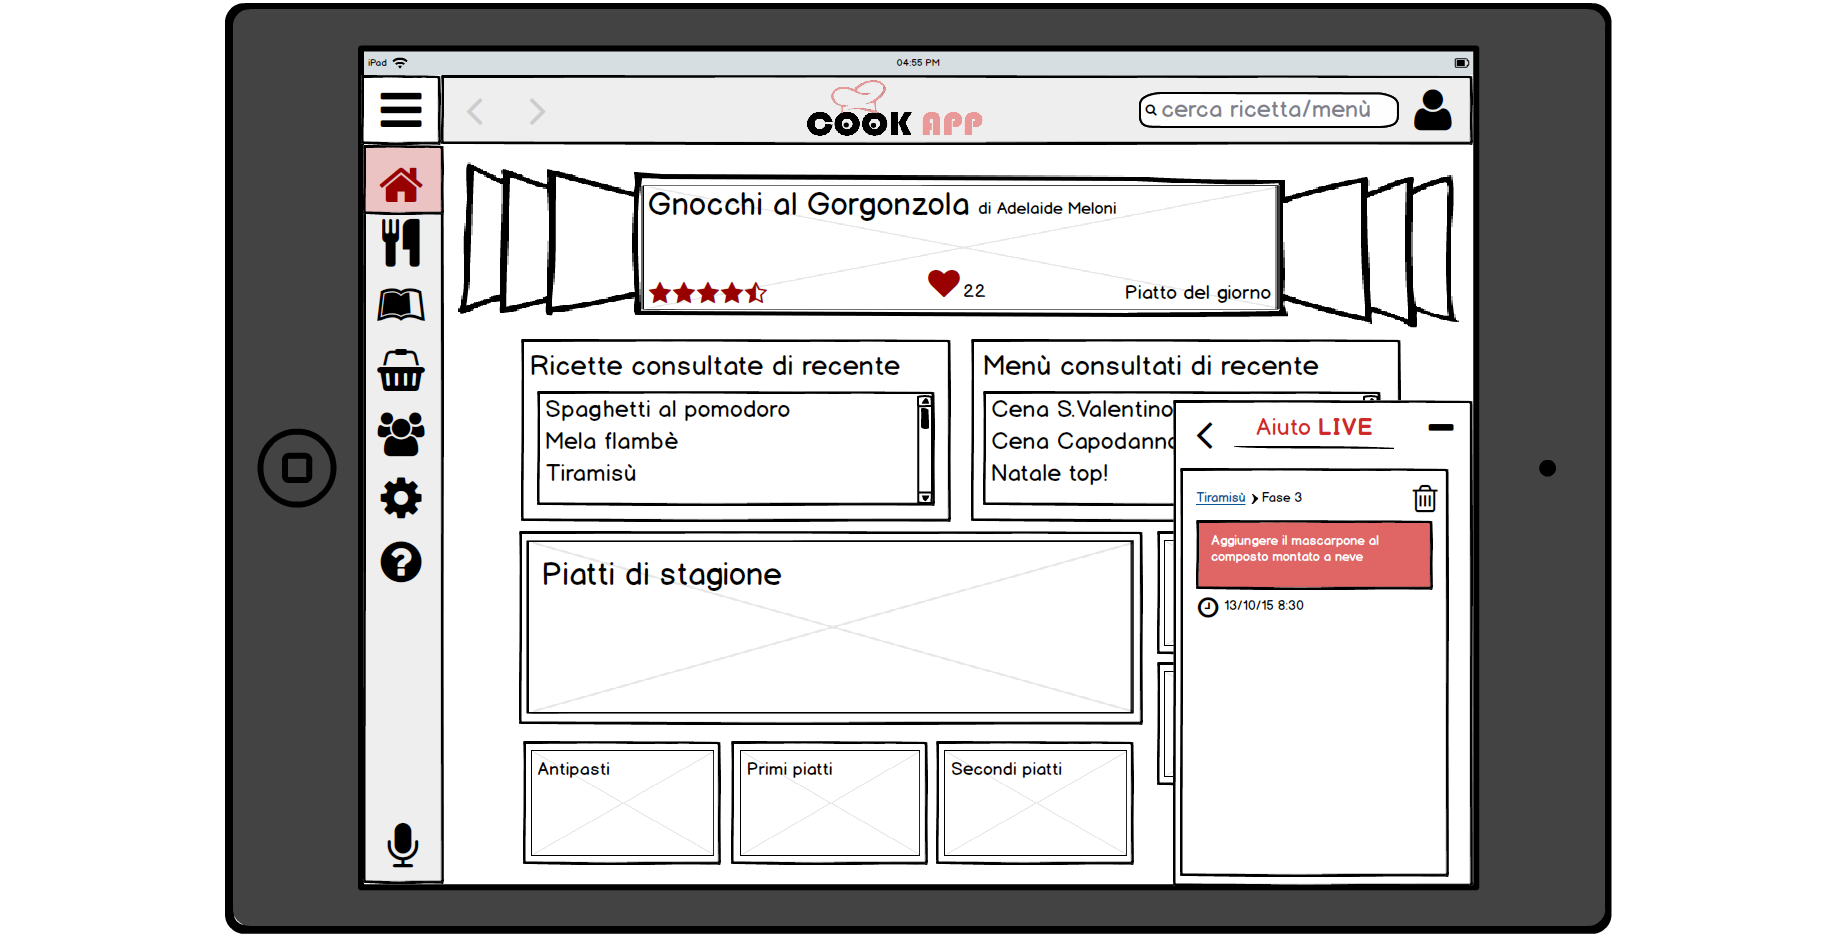
\includegraphics[width=0.95\linewidth]{img/mockup/Live2.png}
\end{figure}
\begin{figure}[H]
	\centering
	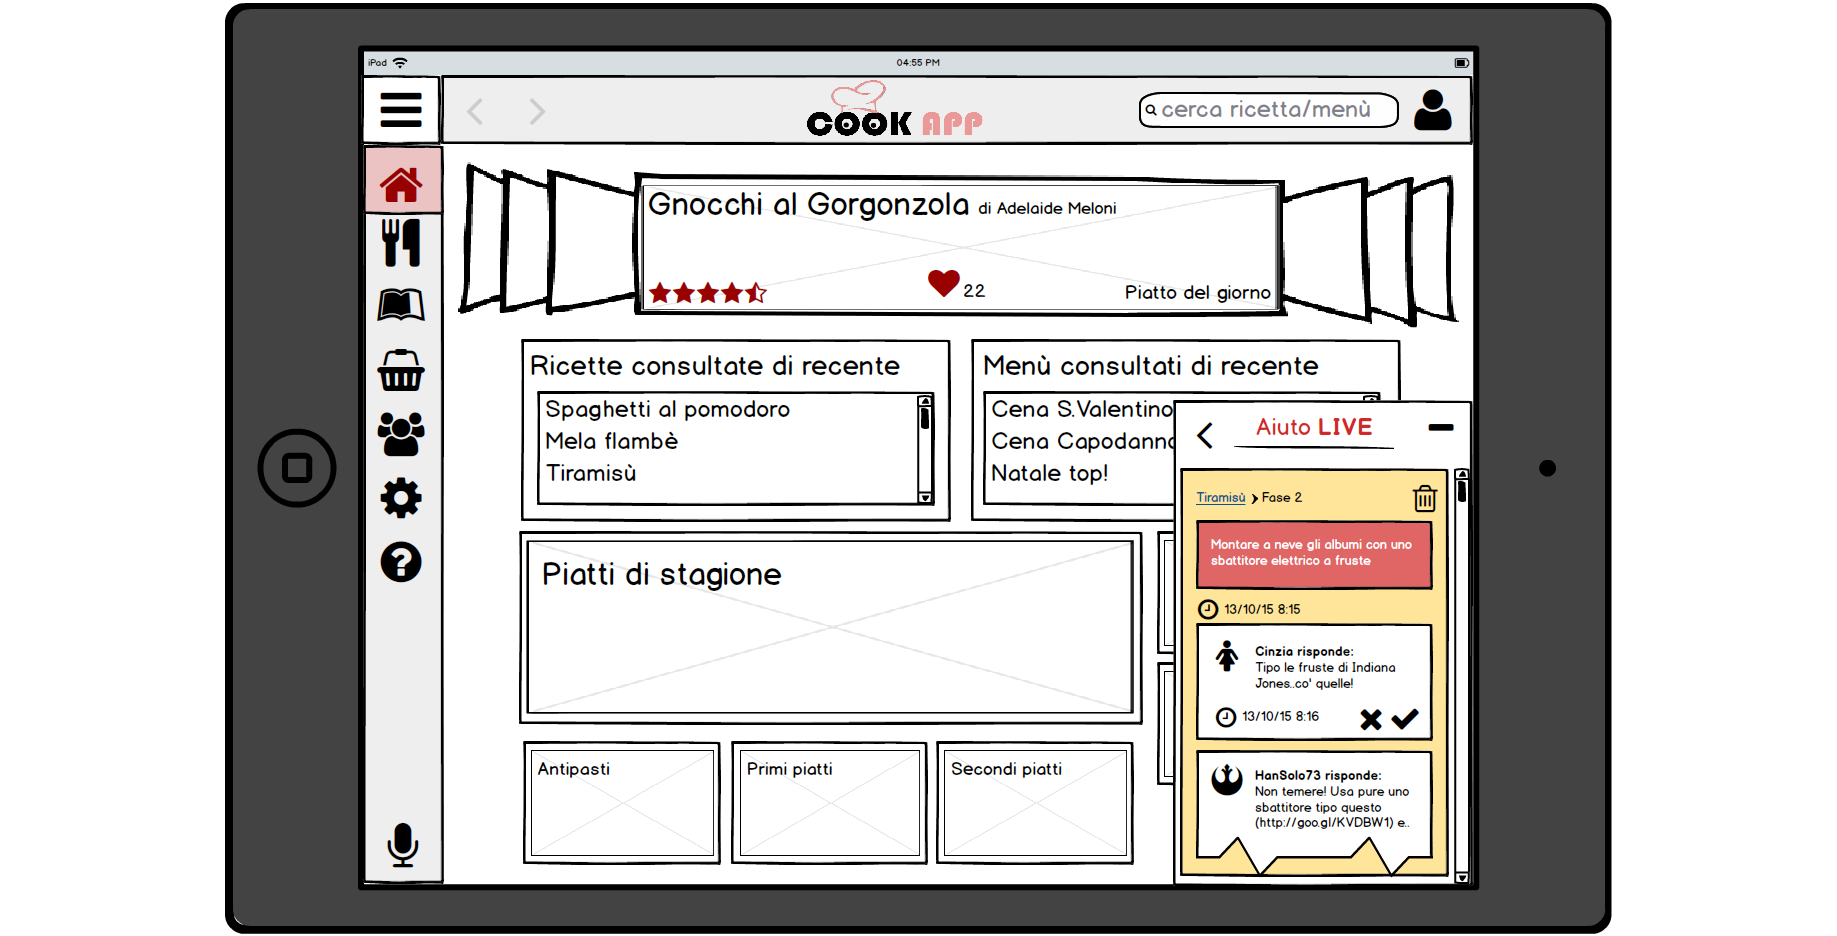
\includegraphics[width=0.95\linewidth]{img/mockup/Live3.png}
\end{figure}
\begin{figure}[H]
	\centering
	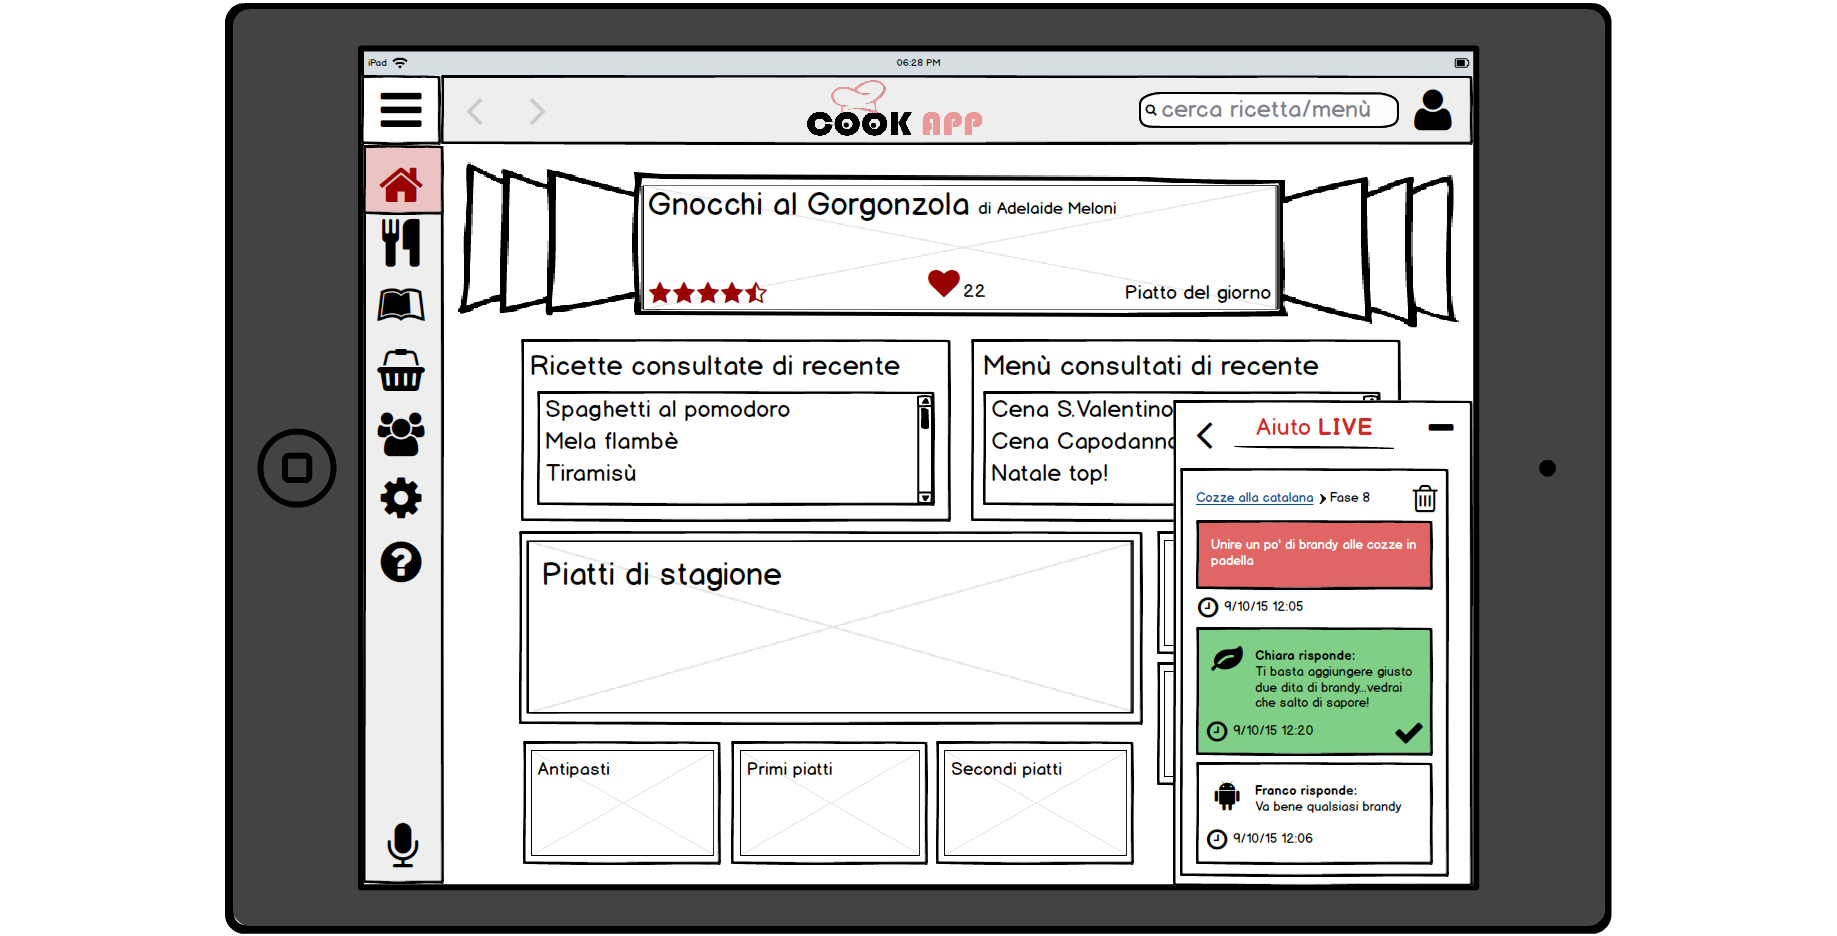
\includegraphics[width=0.95\linewidth]{img/mockup/Live4.png}
\end{figure}

\subsubsection{Ricettario}
Il ricettario è il cuore dell'intero catalogo di CookApp: svariate categorie sono presentate all'utente disposte in un design a mosaico. Le categorie più gettonate tendono a coprire un'area maggiore rispetto alle ricette meno selezionate dalla comunità.\\
Con un semplice tocco delle dita è possibile aprire ogni categoria per ottenere la lista delle ricette.\\
L'utente è inoltre invitato a inserire una propria ricetta mediante l'apposito pulsante oppure può filtrare i risultati visibili cliccando sul simbolo dell'imbuto.\\\\

Ogni categoria mostra le ricette disposte in ordine alfabetico (se l'ordinamento è attivo) ed è possibile già individuare eventuali ricette vegetariane o vegane dall'apposito simbolo presente nei riquadri.\\
L'apposito filtro permette di selezionare determinate tipologie di ricette, in base agli ingredienti presenti, facendo anche particolarmente attenzione a diete particolari e all'intolleranza al lattosio e al glutine. Ulteriori parametri sui quali è possibile fare l'operazioni di filtro sono il tempo il preparazione e le variante vegatariane e vegane di piatti simili.\\
L'opzione "Cos'hai in frigo" è appositamente studiata in CookApp per collegarsi con i modelli più moderni di smartFridge: la sincronizzazione cloud con il frigorifero permetterà di filtrare i risultati in base ai prodotti freschi presenti nel frigo. L'opzione è ovviamente disabilitata se non è presente uno smartFridge collegato.\\
\begin{figure}[H]
	\centering
	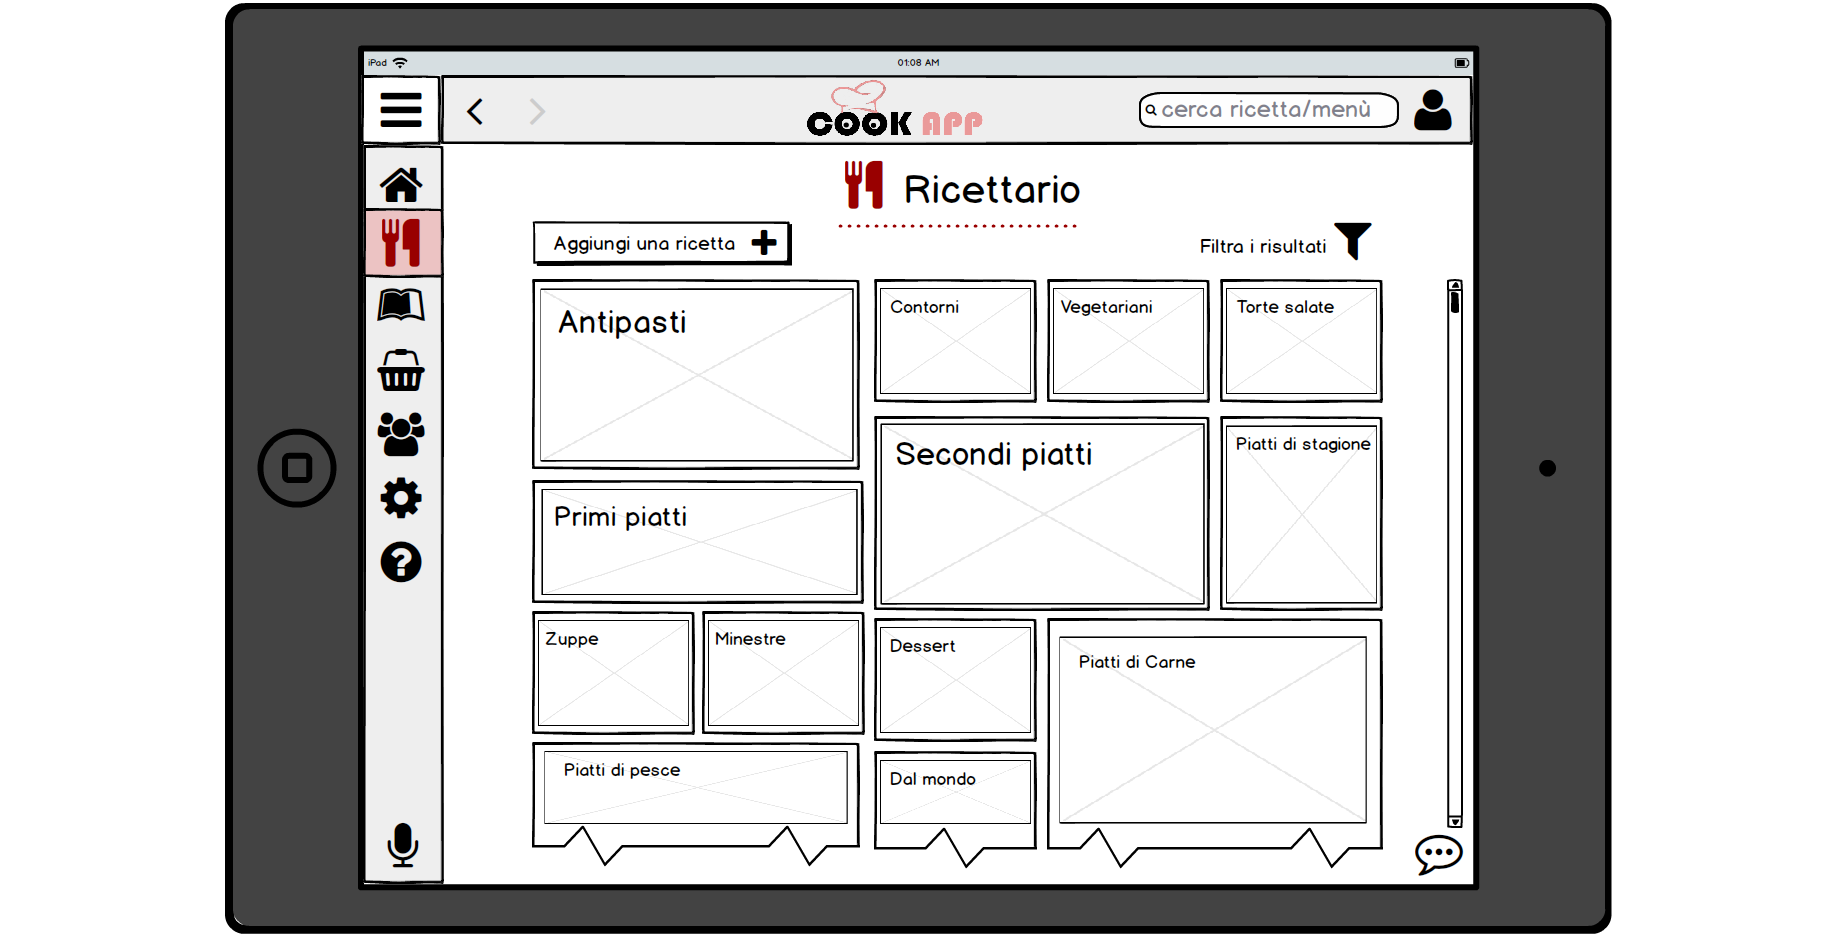
\includegraphics[width=0.95\linewidth]{img/mockup/Ricettario.png}
\end{figure}
\begin{figure}[H]
	\centering
	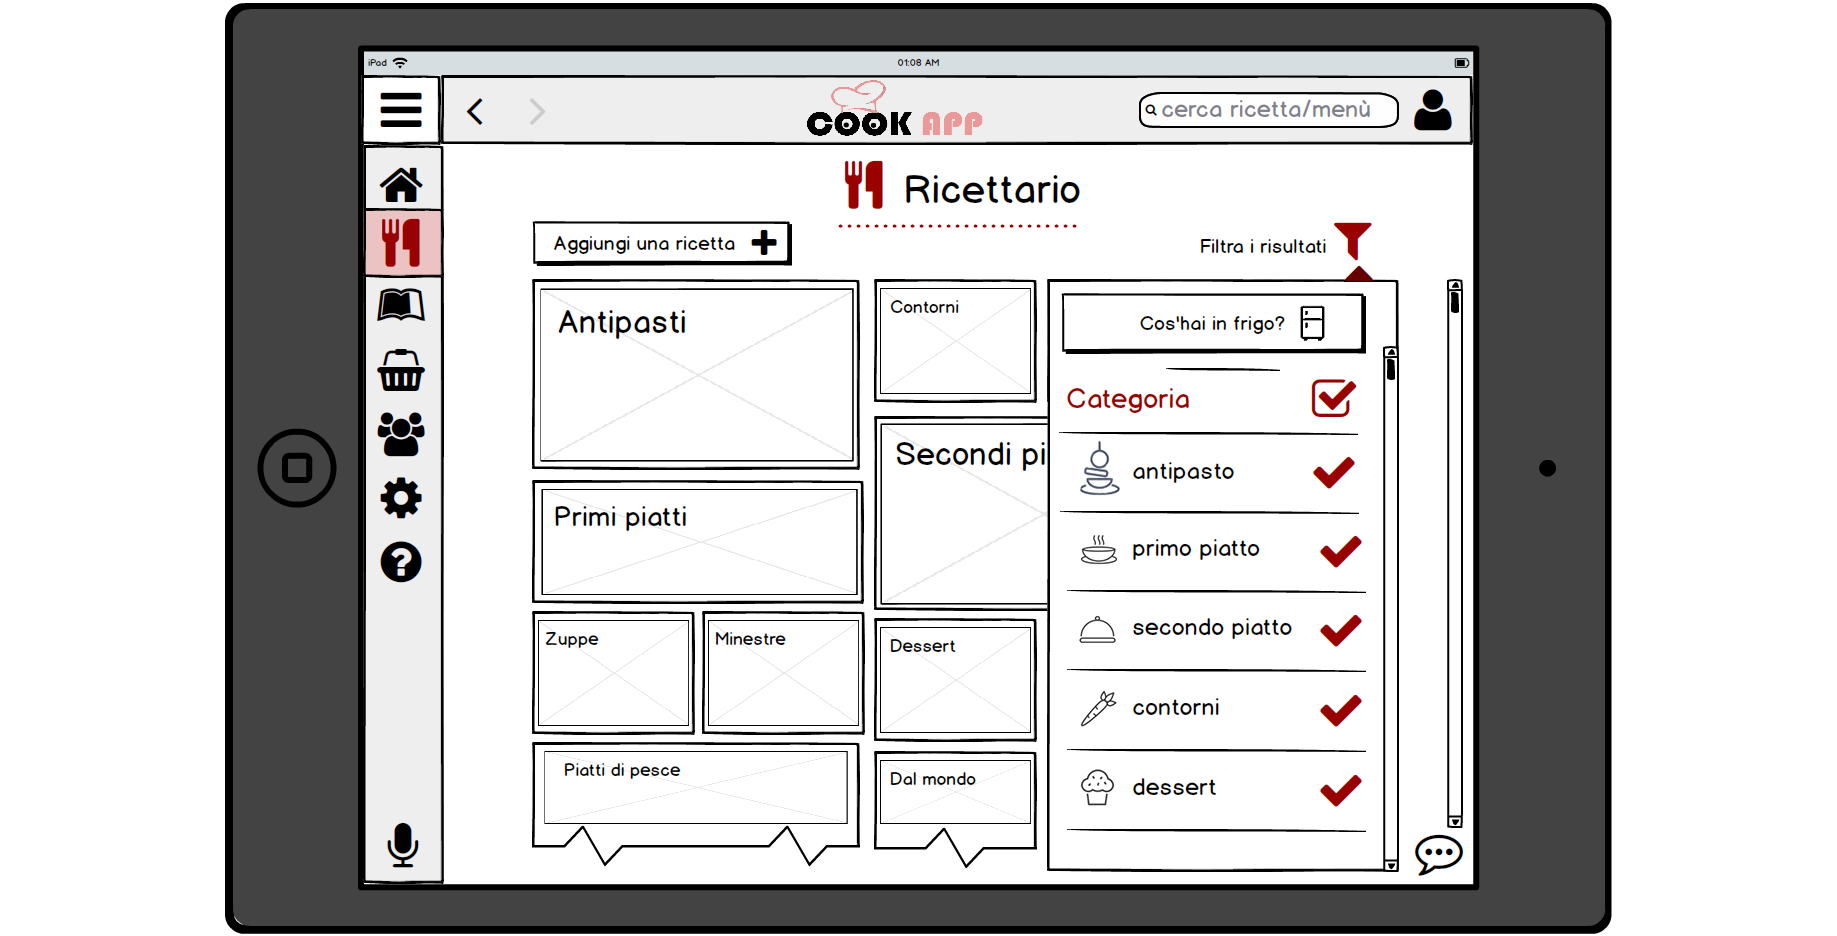
\includegraphics[width=0.95\linewidth]{img/mockup/Ricettario-filtro.png}
\end{figure}
\begin{figure}[H]
	\centering
	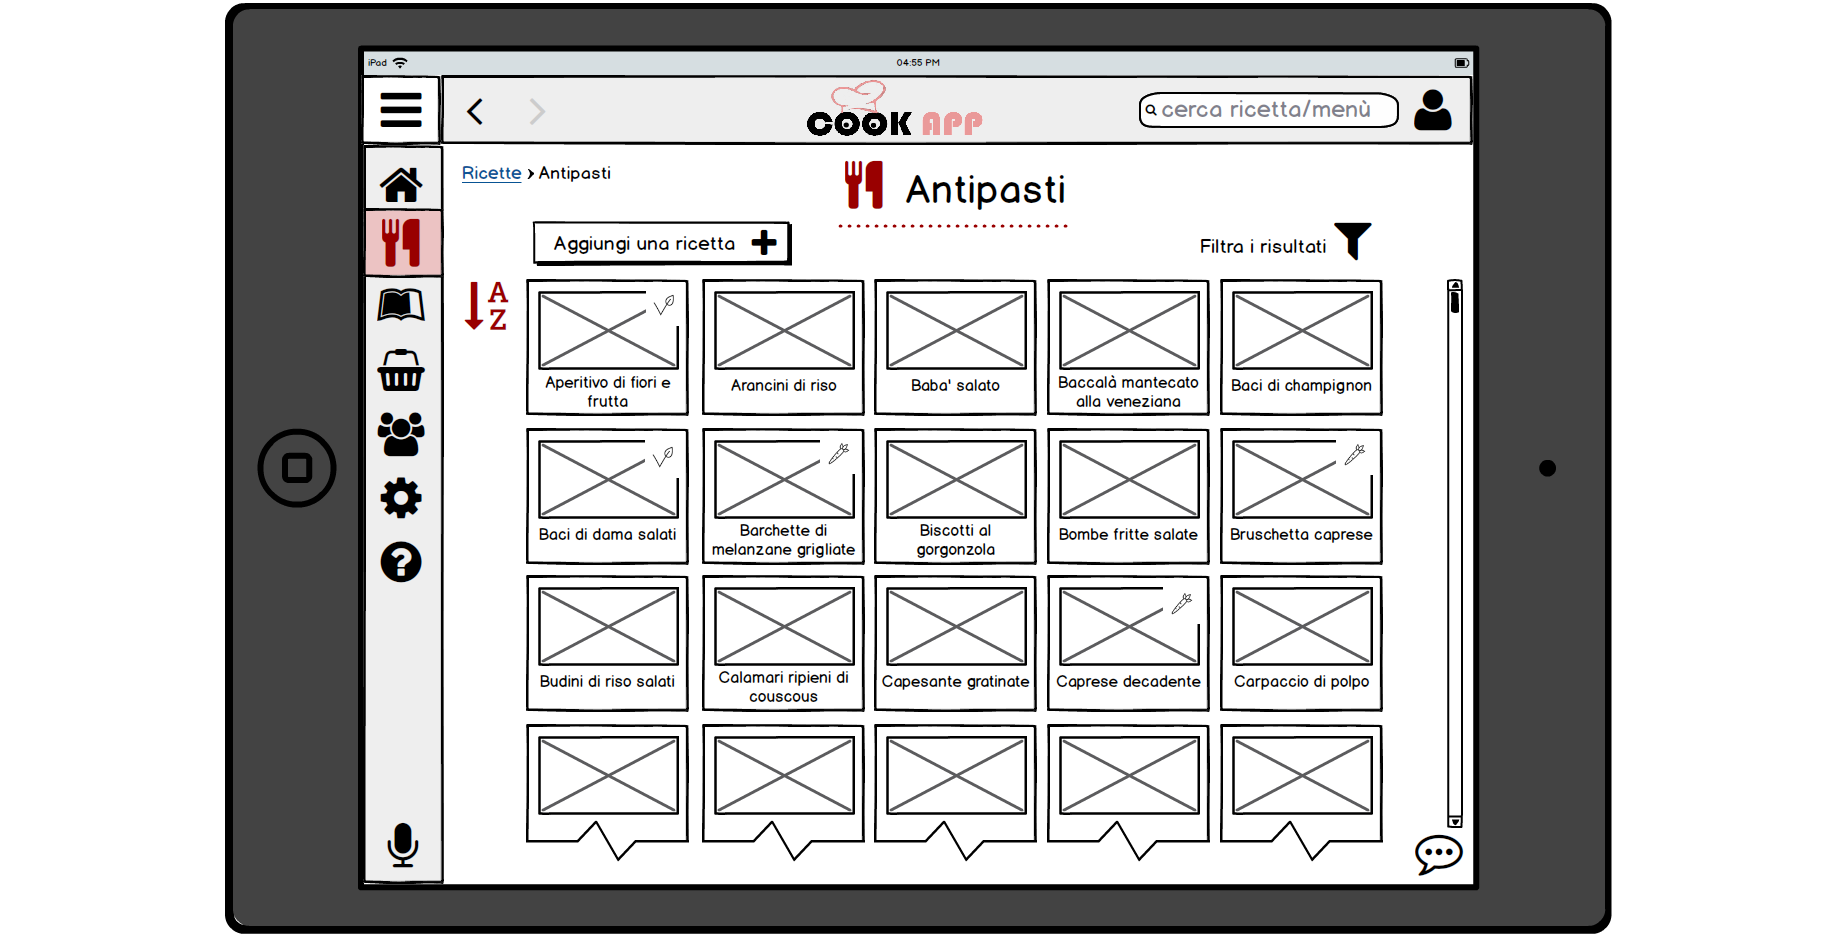
\includegraphics[width=0.95\linewidth]{img/mockup/Ricettario-antipasti.png}
\end{figure}
\begin{figure}[H]
	\centering
	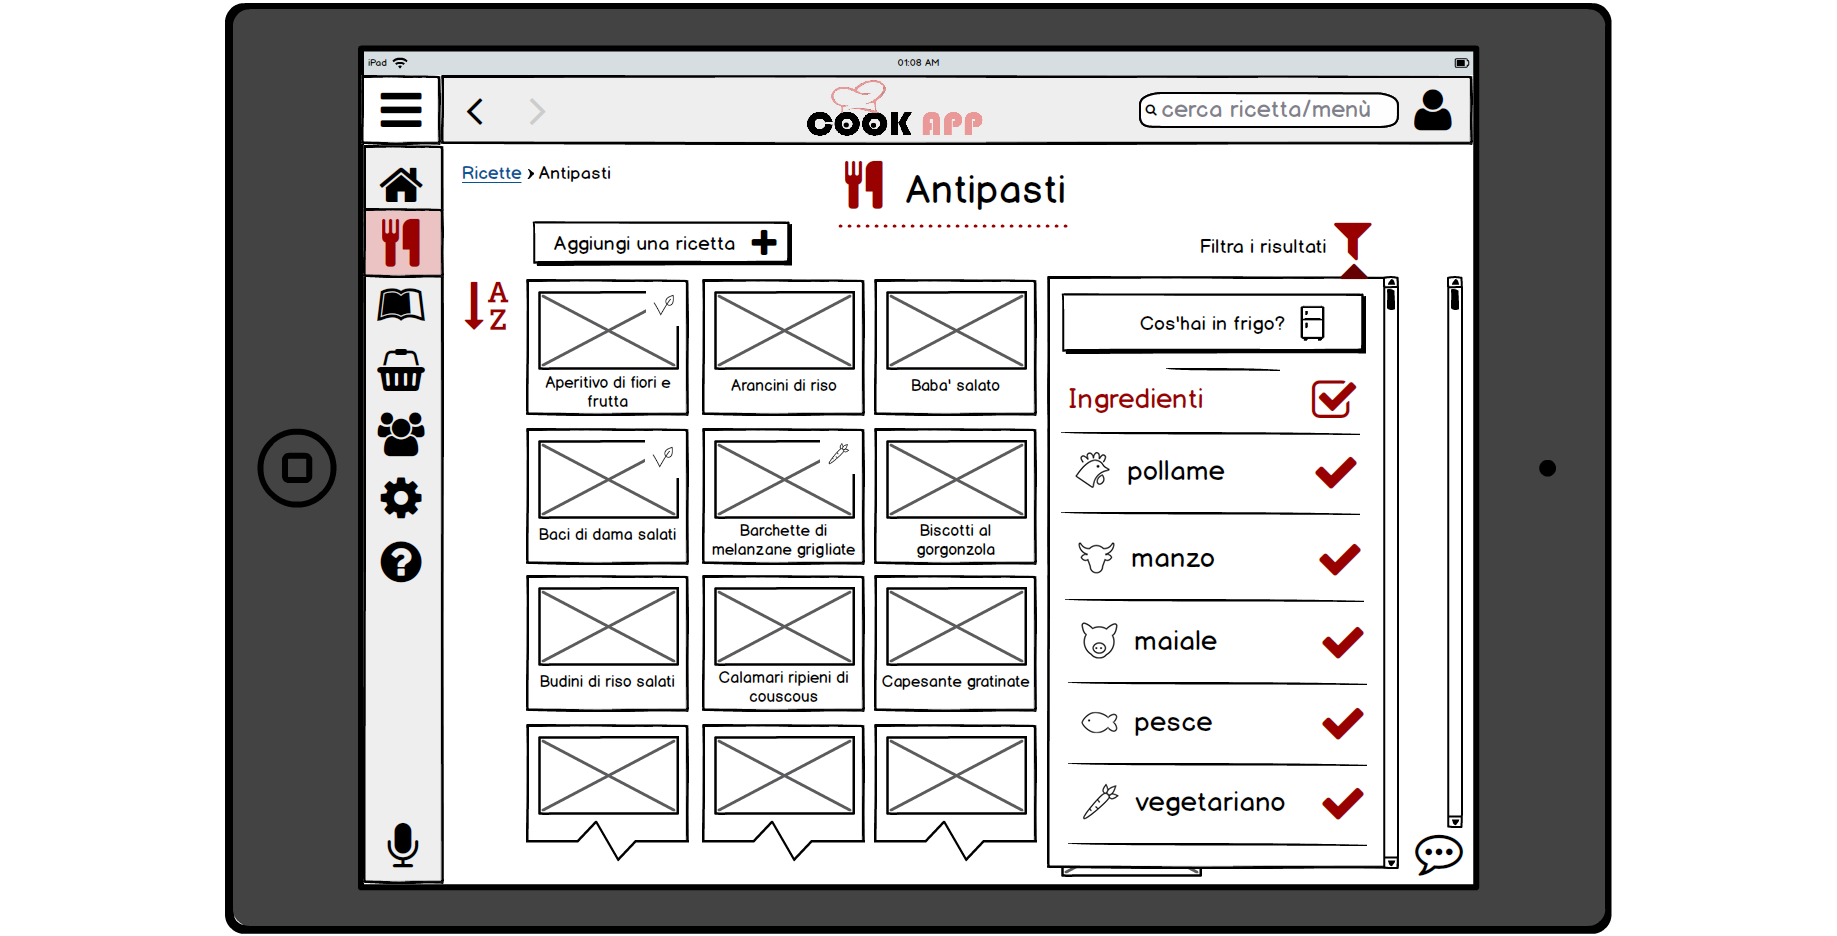
\includegraphics[width=0.95\linewidth]{img/mockup/Ricettario-antipasti-filtro.png}
\end{figure}
\begin{figure}[H]
	\centering
	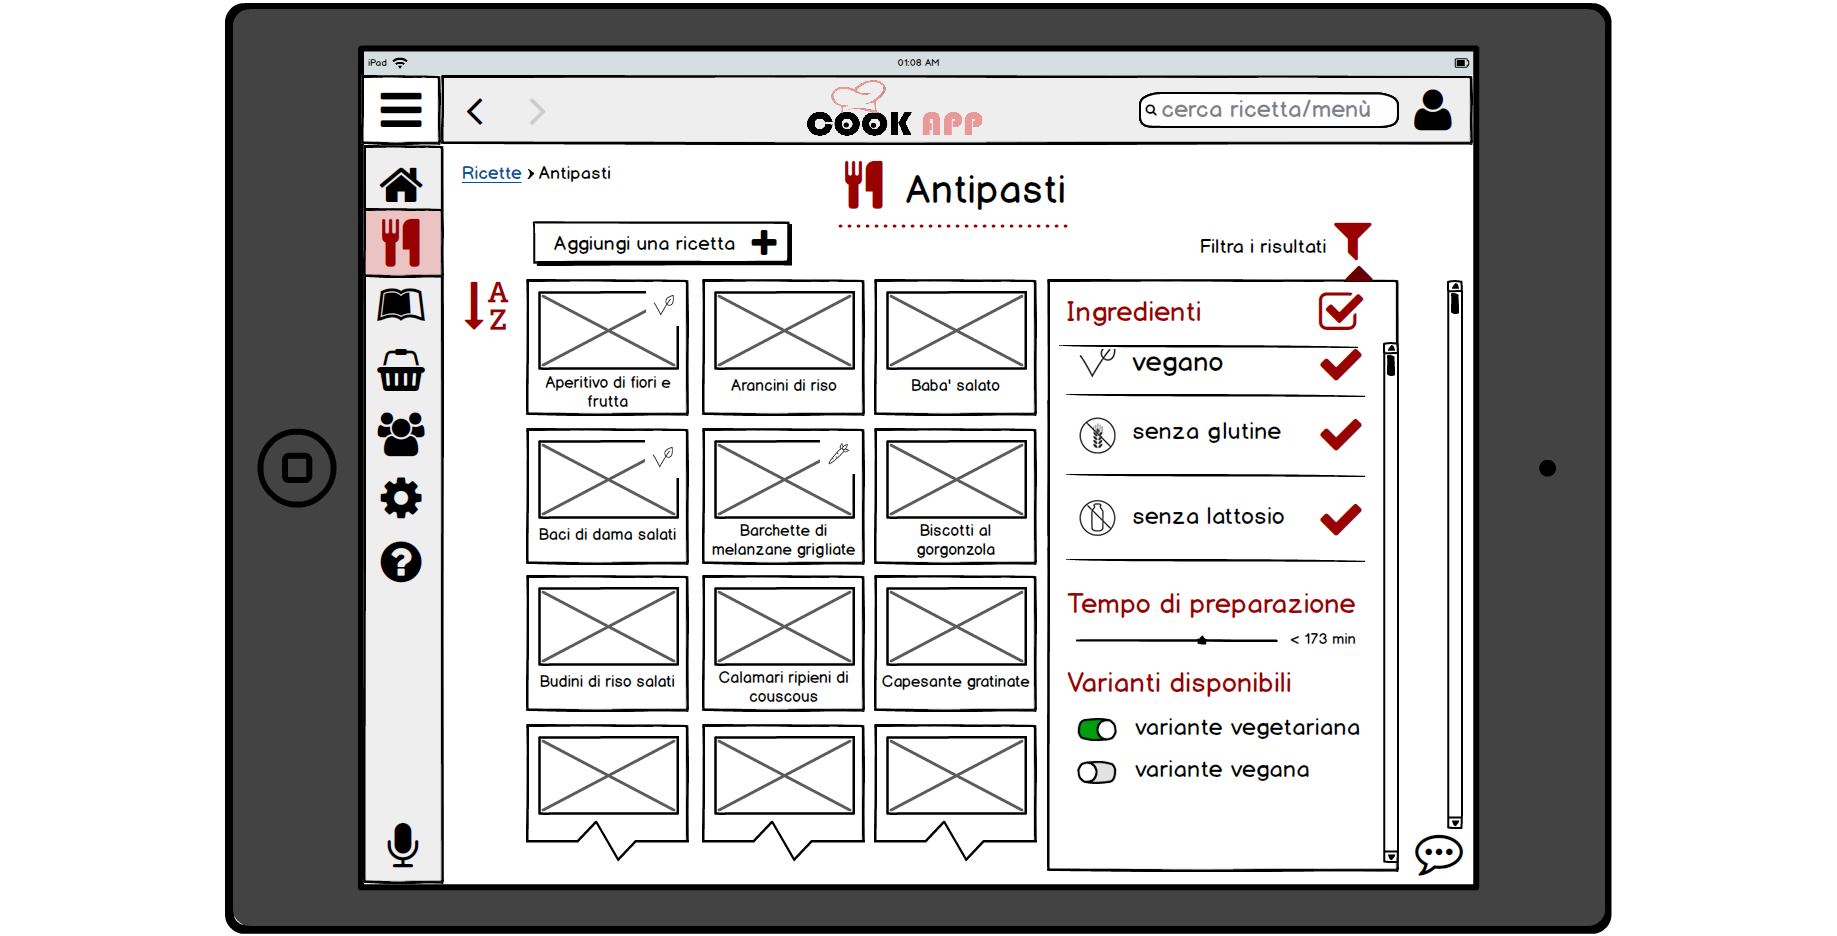
\includegraphics[width=0.95\linewidth]{img/mockup/Ricettario-antipasti-filtro2.png}
\end{figure}
\begin{figure}[H]
	\centering
	
\includegraphics[width=0.95\linewidth]{img/mockup/Ricettario-antipasti-filtro3.png}
\end{figure}

\subsubsection{Ricetta}
Ogni ricetta presenta una lunga schermata visualizzabile mediante lo swipe verticale della pagina.\\
Il banner iniziale mostra la fotografia di copertina della ricetta scelta dall'utente, insieme alla votazione media delle recensioni espressa su 5 stelle e alla possibilità di eliminare la ricetta dal catalogo se si è l'autore.\\
Tempo di preparazione, di cottura, difficoltà di realizzazione e costo delle materie prime, sono ben visibili affianco alla galleria di fotografie della ricette; sempre qui è inoltre possibile sapere quanti utenti hanno aggiunto la ricetta ai propri preferiti.\\
La sezione successiva mostra le varie quantità di ingredienti necessari, in sistema metrico (se non diversamente richiesto nelle impostazioni) e permette di adeguare ogni quantità in base alle persone richieste. Tramite l'apposito pulsante è possibile aggiungere tutti gli ingredienti, automaticamente, nella lista della spesa, raggiungibile cliccando sul quarto simbolo a sinistra.\\
La fase di preparazione mostra 3 diverse tipologie di vista, per soddisfare ogni tipologia di utente: da quello che necessita più dettagli e aiuti nella preparazione del piatto, al professionista.\\
\begin{enumerate}
\item La vista "Passo-passo 3D" è una nuova funzionalità esclusiva che permette di interagire a 360 gradi con una riproduzione 3D del piatto che si sta preparando. Ogni fase è accompagnata da un'animazione in tre dimensioni, che permette di verificare la corretta procedura su più punti di visione.
\item La vista "Passo-passo video" affianca la descrizione testuale della ricetta alla visione di un video che mostra la procedura tramite il player. Il sistema è ottimizzato per sincronizzare il tempo di riproduzione del video e la fase del procedimento corrispondente.
\item La "Vista compatta" è quella classica, dove vengono mostrate tutte le fasi di preparazione, lasciando all'utente il compito di sincronizzare lavoro e testo scritto.
\end{enumerate}
Ogni step di preparazione mostra sempre la possibilità di chiedere alla community, aiuto riguardo quel preciso passaggio. Automaticamente verrà creata una nuova voce della sezione "Aiuti live" già descritta in precedenza.\\
Nelle ultime sezioni vi sono i pulsanti di interazione con la ricetta: è qui possibile aggiungere la ricetta ai preferiti, aggiungere la ricetta ad un menù personale (con la possibilità di crearne uno direttamente da qui) e la possibilità di condividere la ricetta sui social network o sui servizi di messaggistica.\\
Infine la sezione "Recensioni" permette sia la scrittura che la lettura delle opinioni di altri utenti sulla ricetta.\\
\begin{figure}[H]
	\centering
	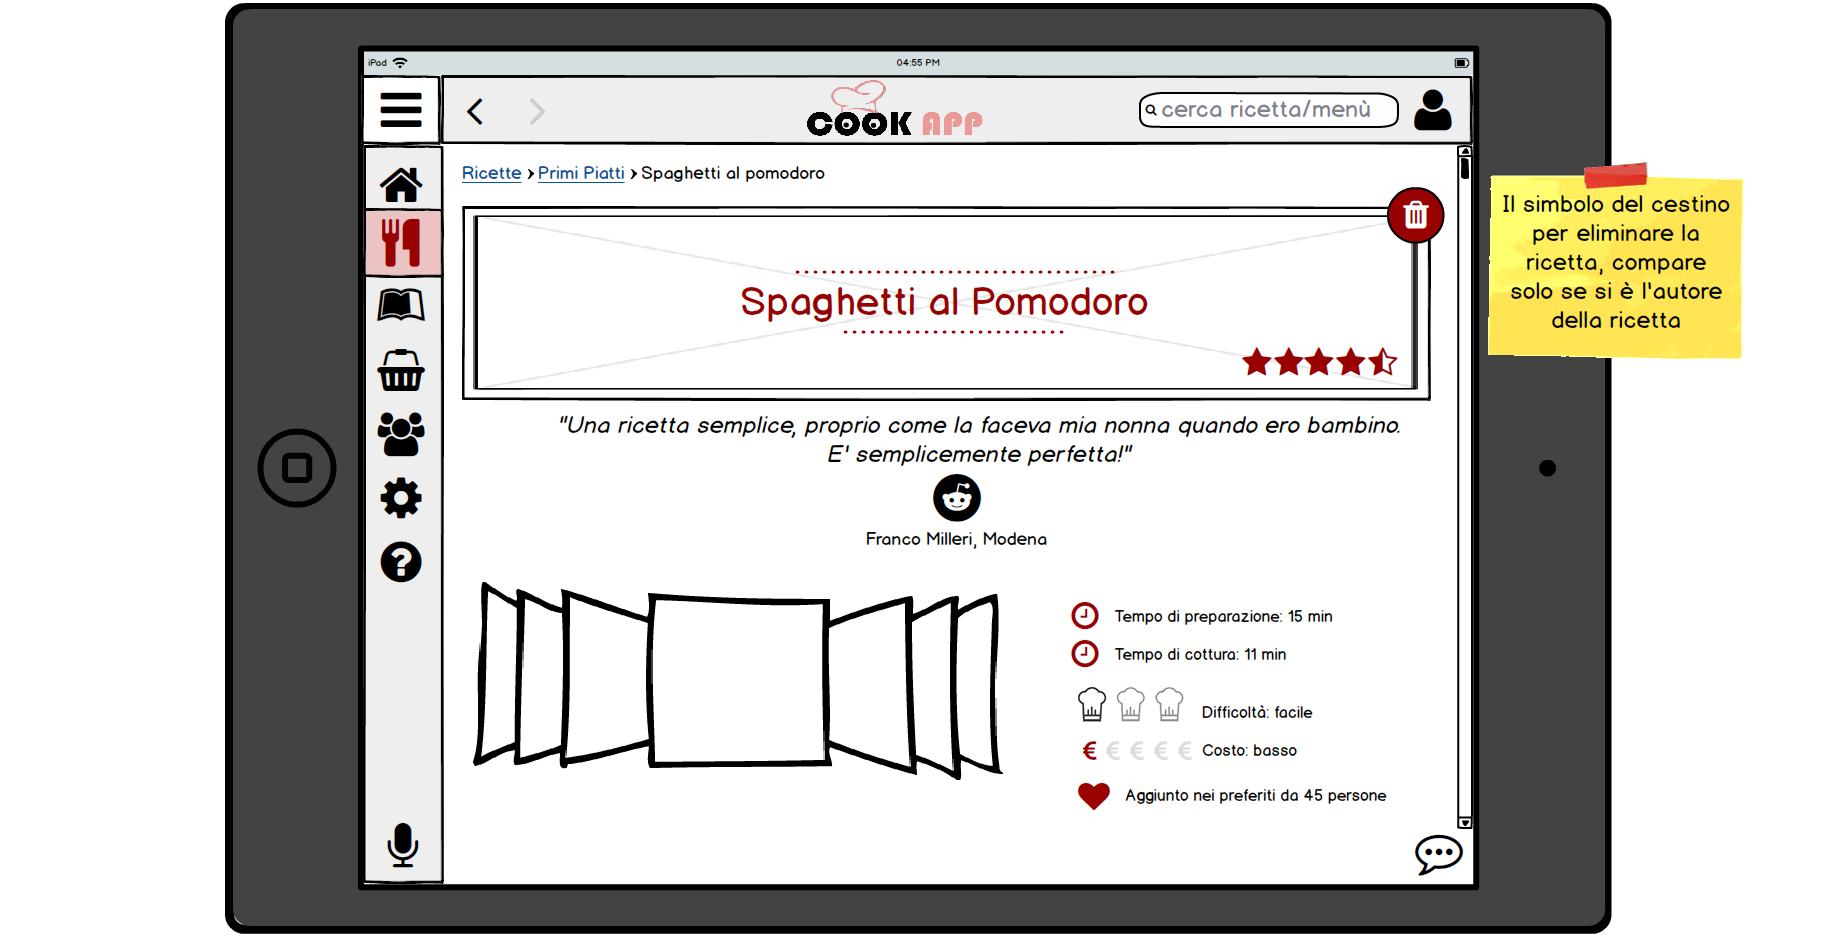
\includegraphics[width=0.95\linewidth]{img/mockup/Ricetta.png}
\end{figure}
\begin{figure}[H]
	\centering
	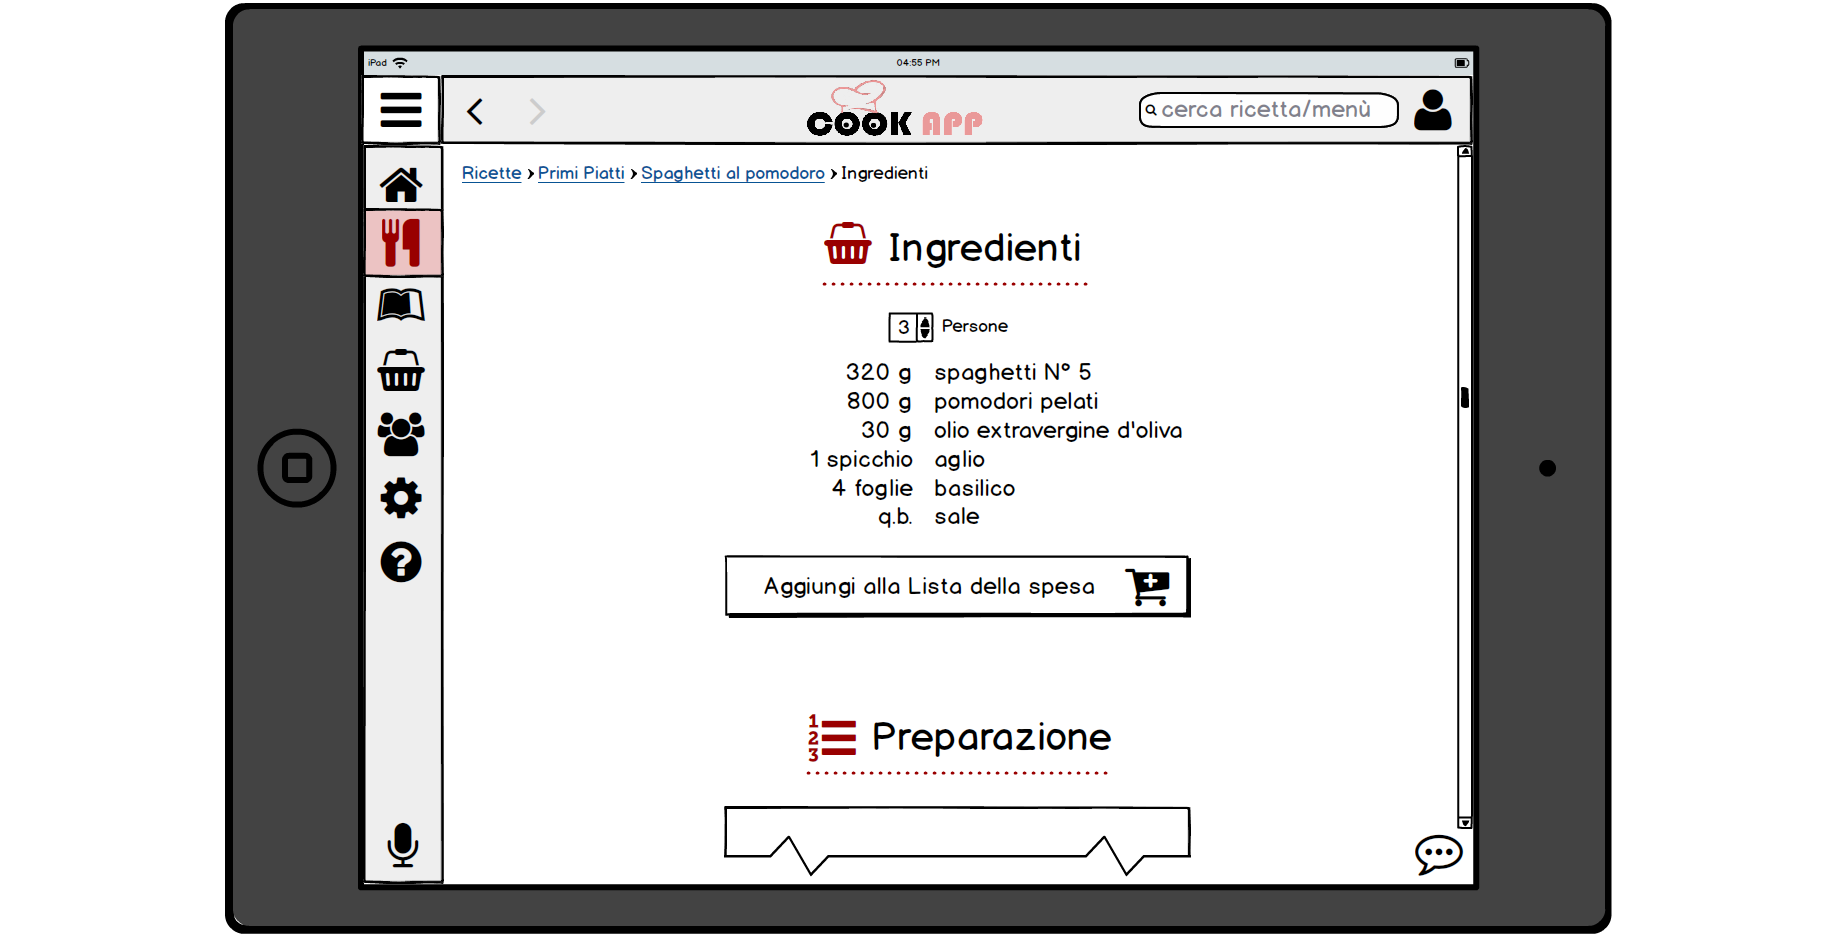
\includegraphics[width=0.95\linewidth]{img/mockup/Ricetta2.png}
\end{figure}
\begin{figure}[H]
	\centering
	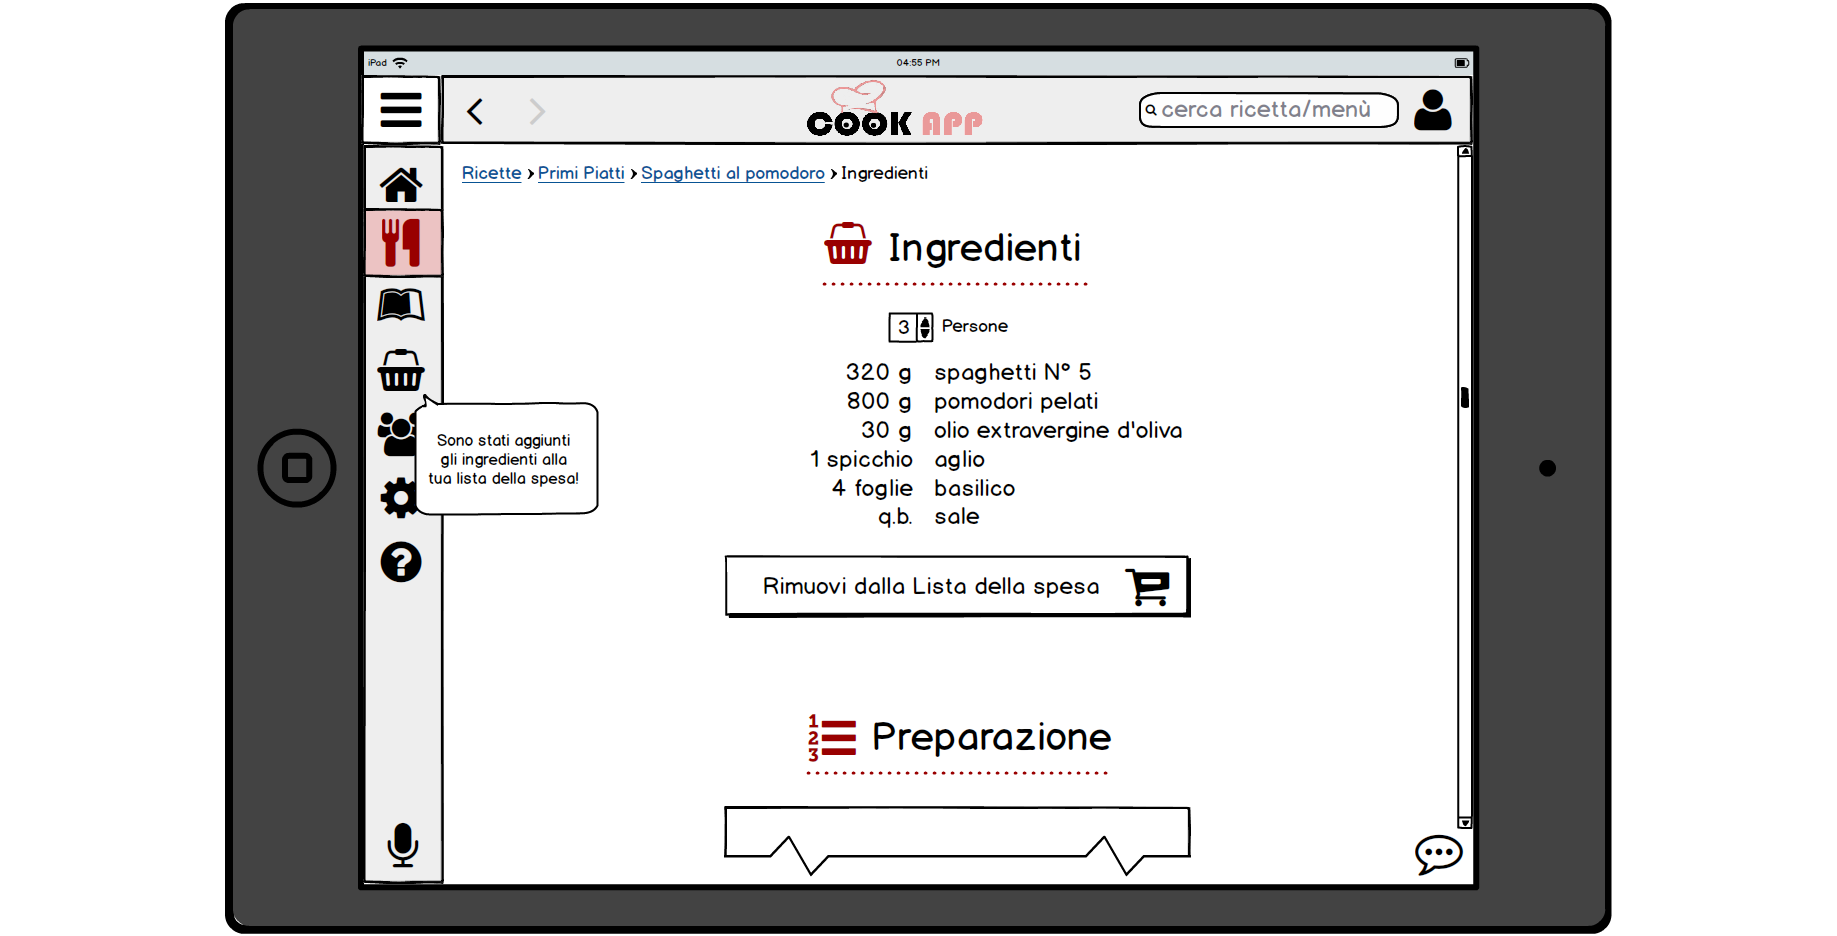
\includegraphics[width=0.95\linewidth]{img/mockup/Ricetta2-spesa.png}
\end{figure}
\begin{figure}[H]
	\centering
	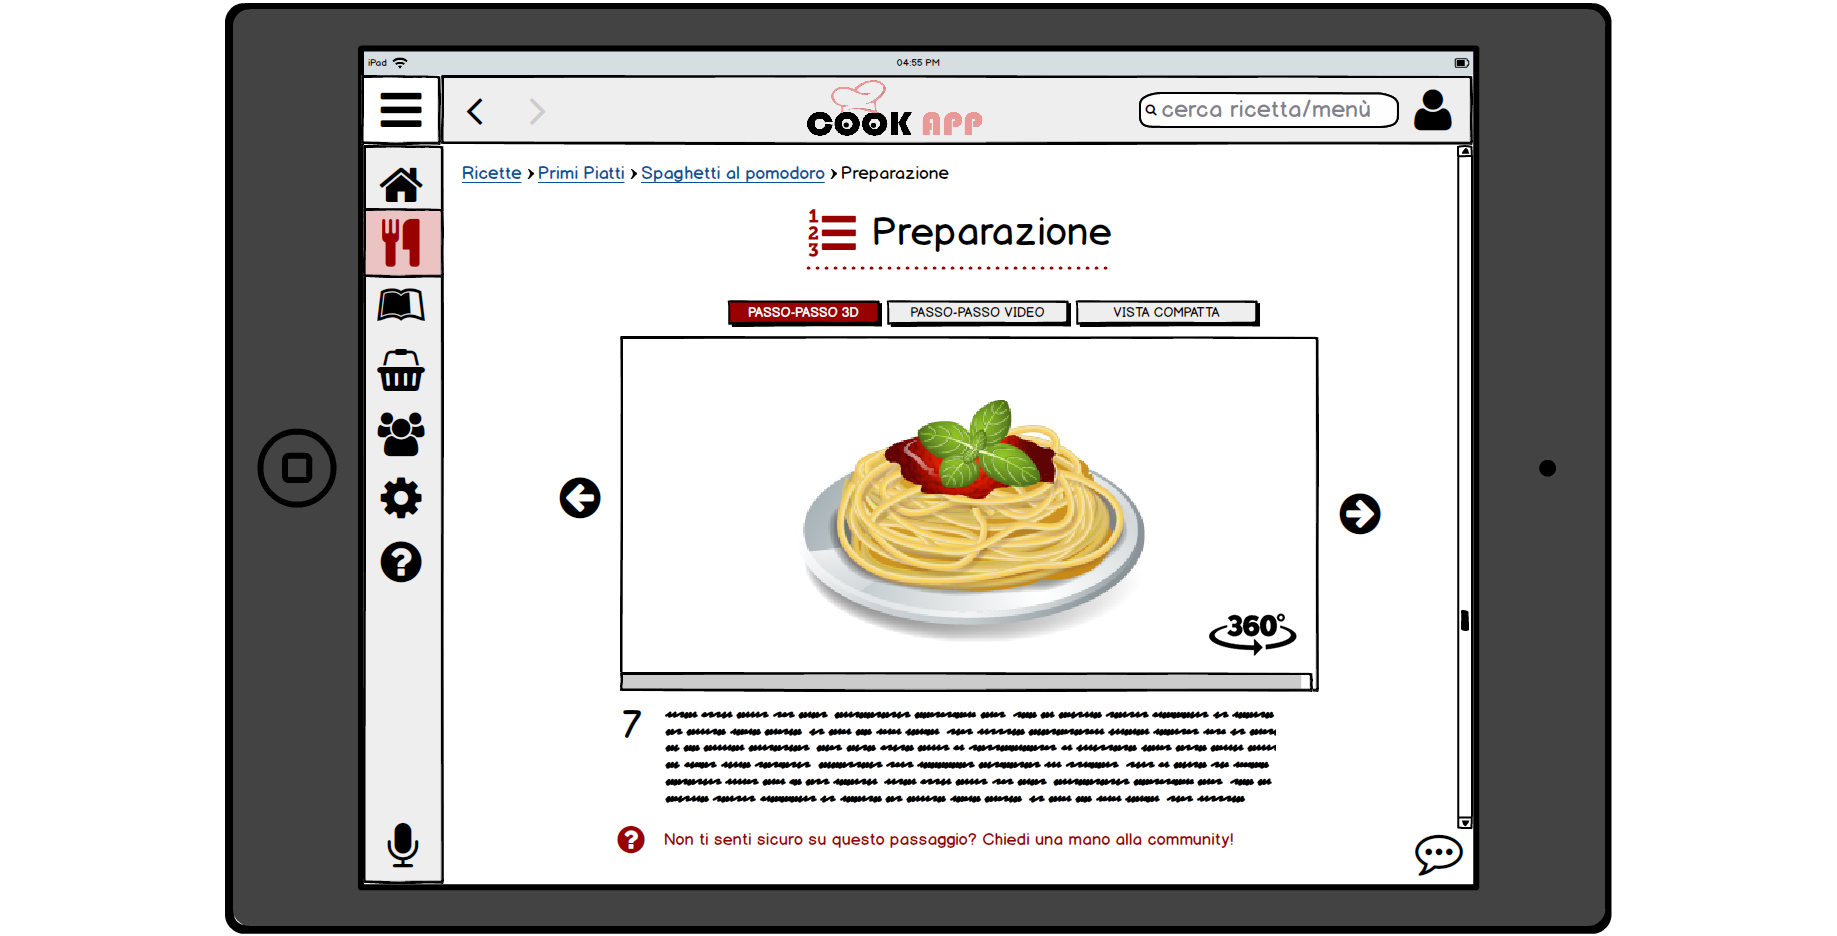
\includegraphics[width=0.95\linewidth]{img/mockup/Ricetta3.png}
\end{figure}
\begin{figure}[H]
	\centering
	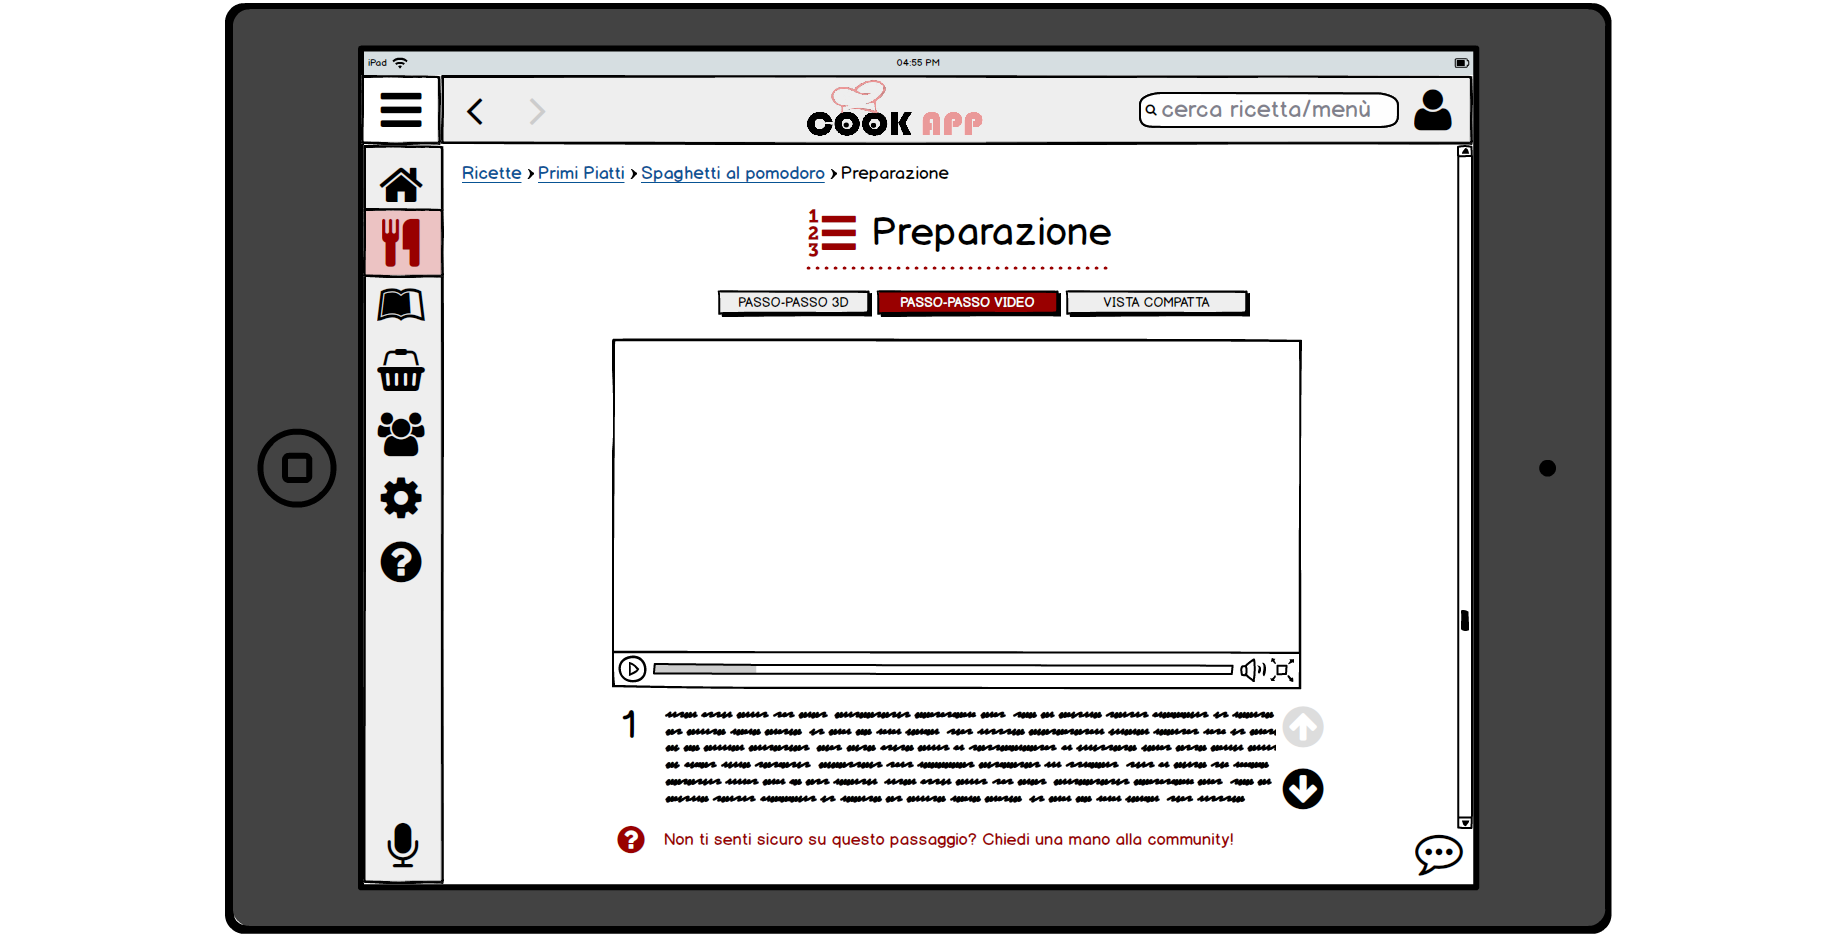
\includegraphics[width=0.95\linewidth]{img/mockup/Ricetta4.png}
\end{figure}
\begin{figure}[H]
	\centering
	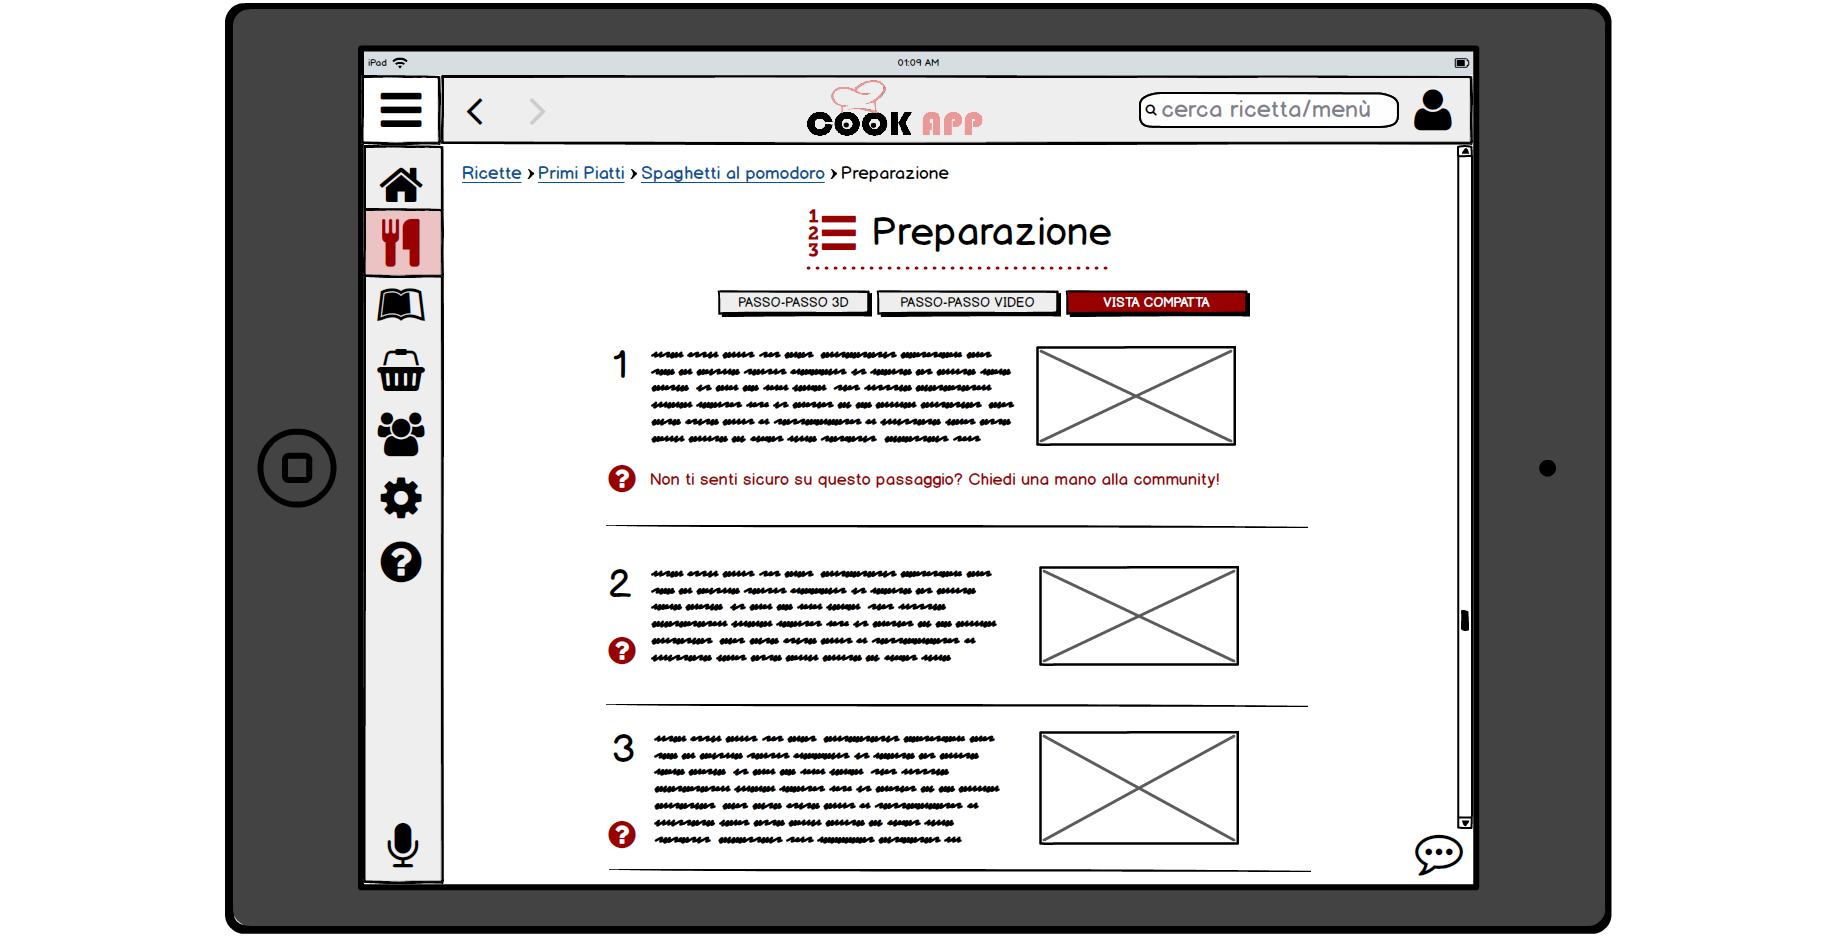
\includegraphics[width=0.95\linewidth]{img/mockup/Ricetta5.png}
\end{figure}
y\begin{figure}[H]
	\centering
	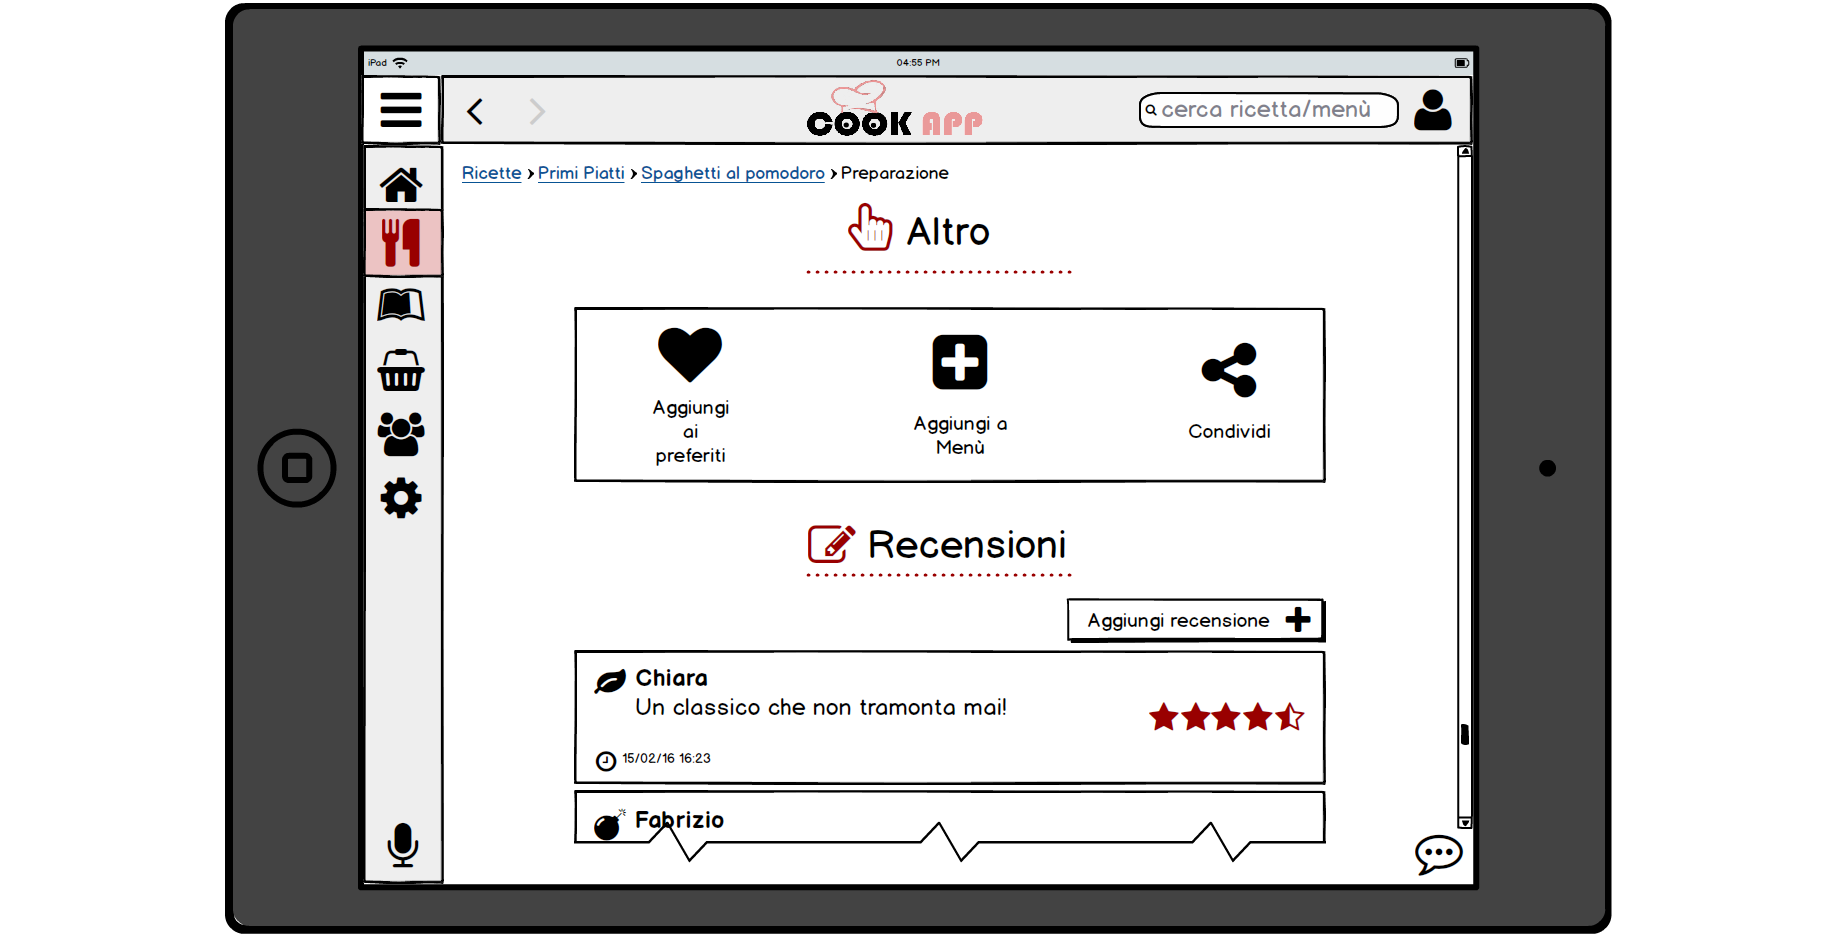
\includegraphics[width=0.95\linewidth]{img/mockup/Ricetta6.png}
\end{figure}
\begin{figure}[H]
	\centering
	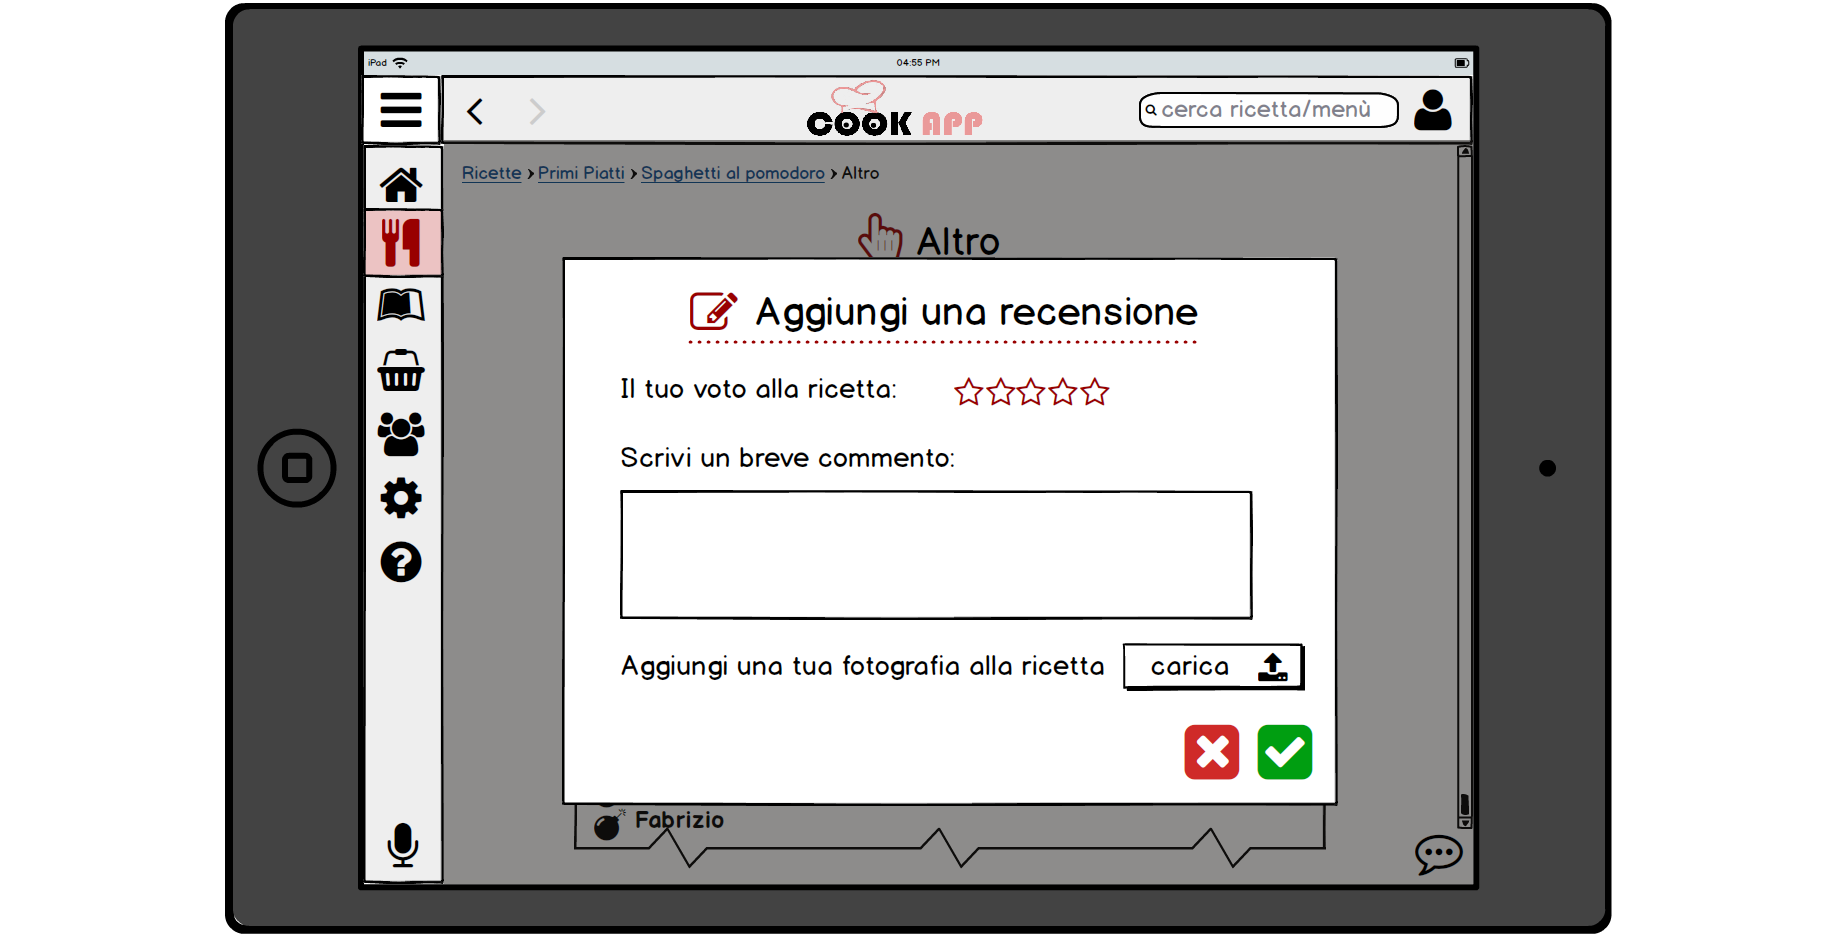
\includegraphics[width=0.95\linewidth]{img/mockup/Ricetta7.png}
\end{figure}
\begin{figure}[H]
	\centering
	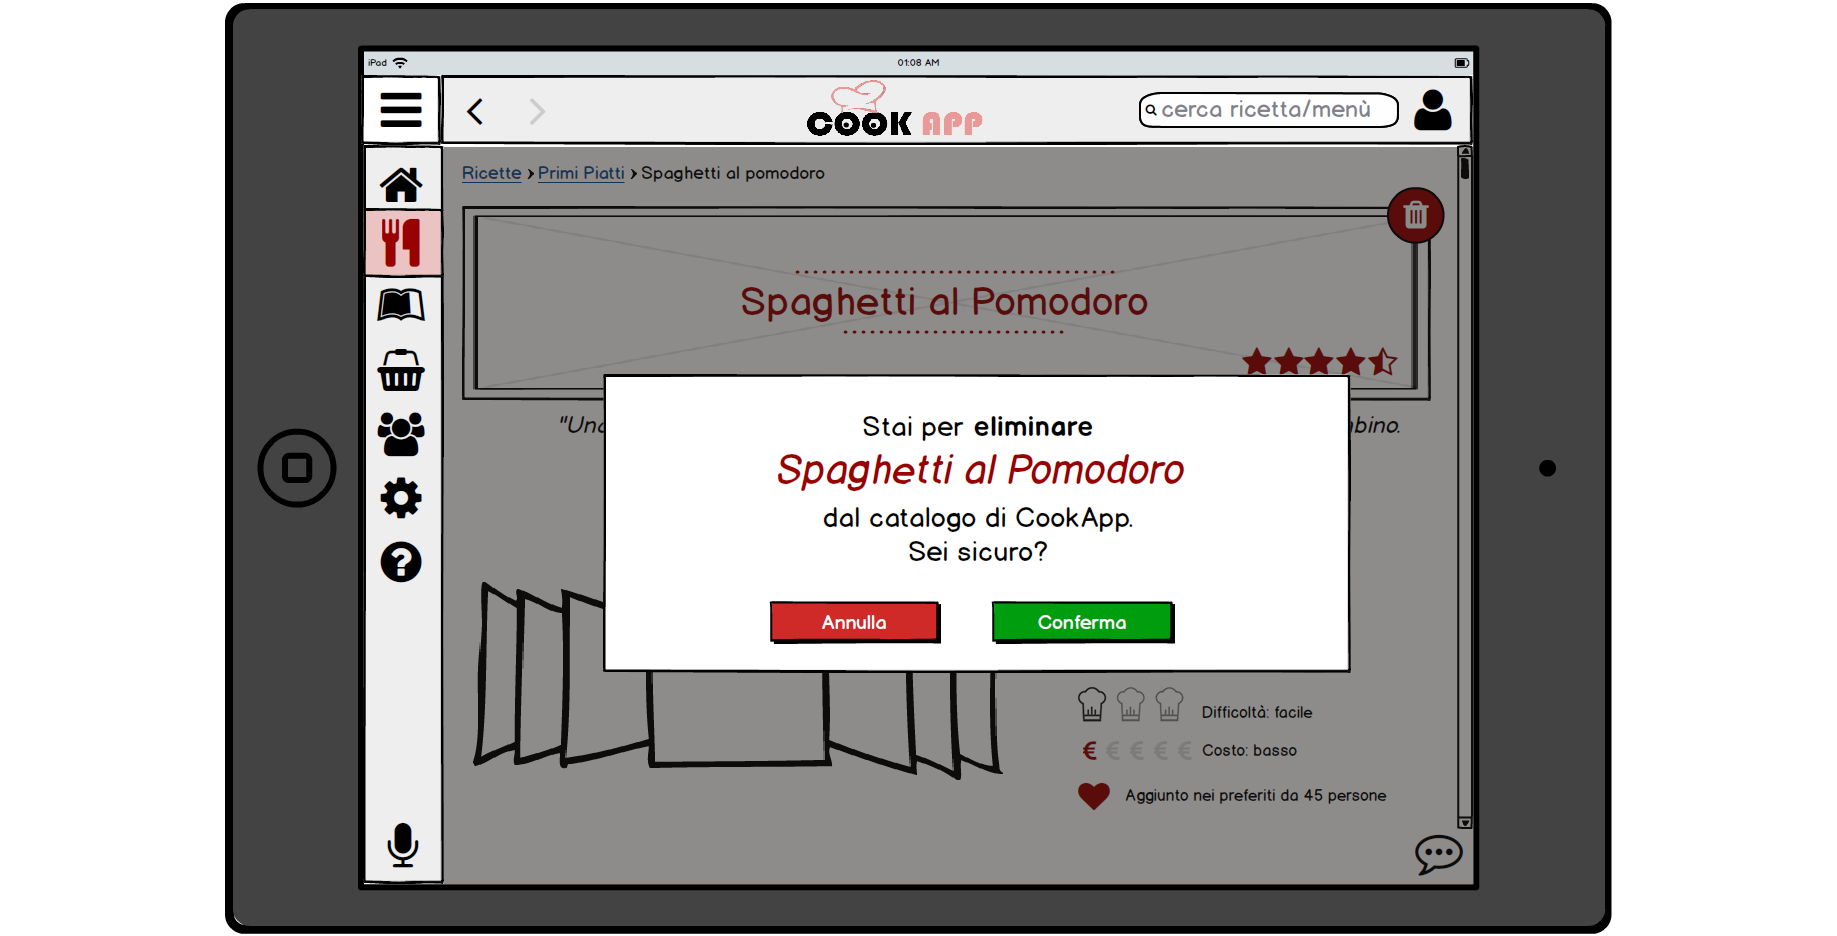
\includegraphics[width=0.95\linewidth]{img/mockup/Ricetta-remove.png}
\end{figure}


\subsubsection{Aggiunta di una ricetta}
Mediante all'apposito pulsante "Aggiungi una ricetta" è possibile arricchire il catalogo di CookApp.\\
Si interagisce quindi con una serie di fasi che guidano passo-passo l'utente all'inserimento di tutte le informazioni necessarie: qui vi si trova la possibilità di inserire tutte i dati visti in precedenza nella sezione "Ricette".\\
Si noti come, nella fase 3, è possibile abbinare a ogni descrizione di fase di preparazione, una fotografia esplicativa o un video. Sempre in questa sezione, il tasto "Aggiungi un'altra fase" permette di inserire qualsiasi numero di step necessari al completamento della ricetta.\\
L'ultima fase, ovvero la quarta, permette all'utente di indicare se il piatto è vegetariano e se è rappresenta una variante a un piatto simile, ma contenente carne. Stessa procedura è prevista se è un piatto vegano.\\
Dopo aver impostato difficoltà, costo e numero di persone, si invita l'utente a inserire un set di tag per classificare correttamente la ricetta: se il tag inserito è riconosciuto dal sistema, verrà visualizzato in un riquadro colorato.\\
Completato l'inserimento di tutti i dati richieste l'utente non deve fare altro che confermare l'inserimento della ricetta.\\
Il sistema conclude l'operazione assegnando un quantitativo di punti esperienza permettendo all'utente di avanzare di livello (vedi sez. Gamification).\\
\begin{figure}[H]
	\centering
	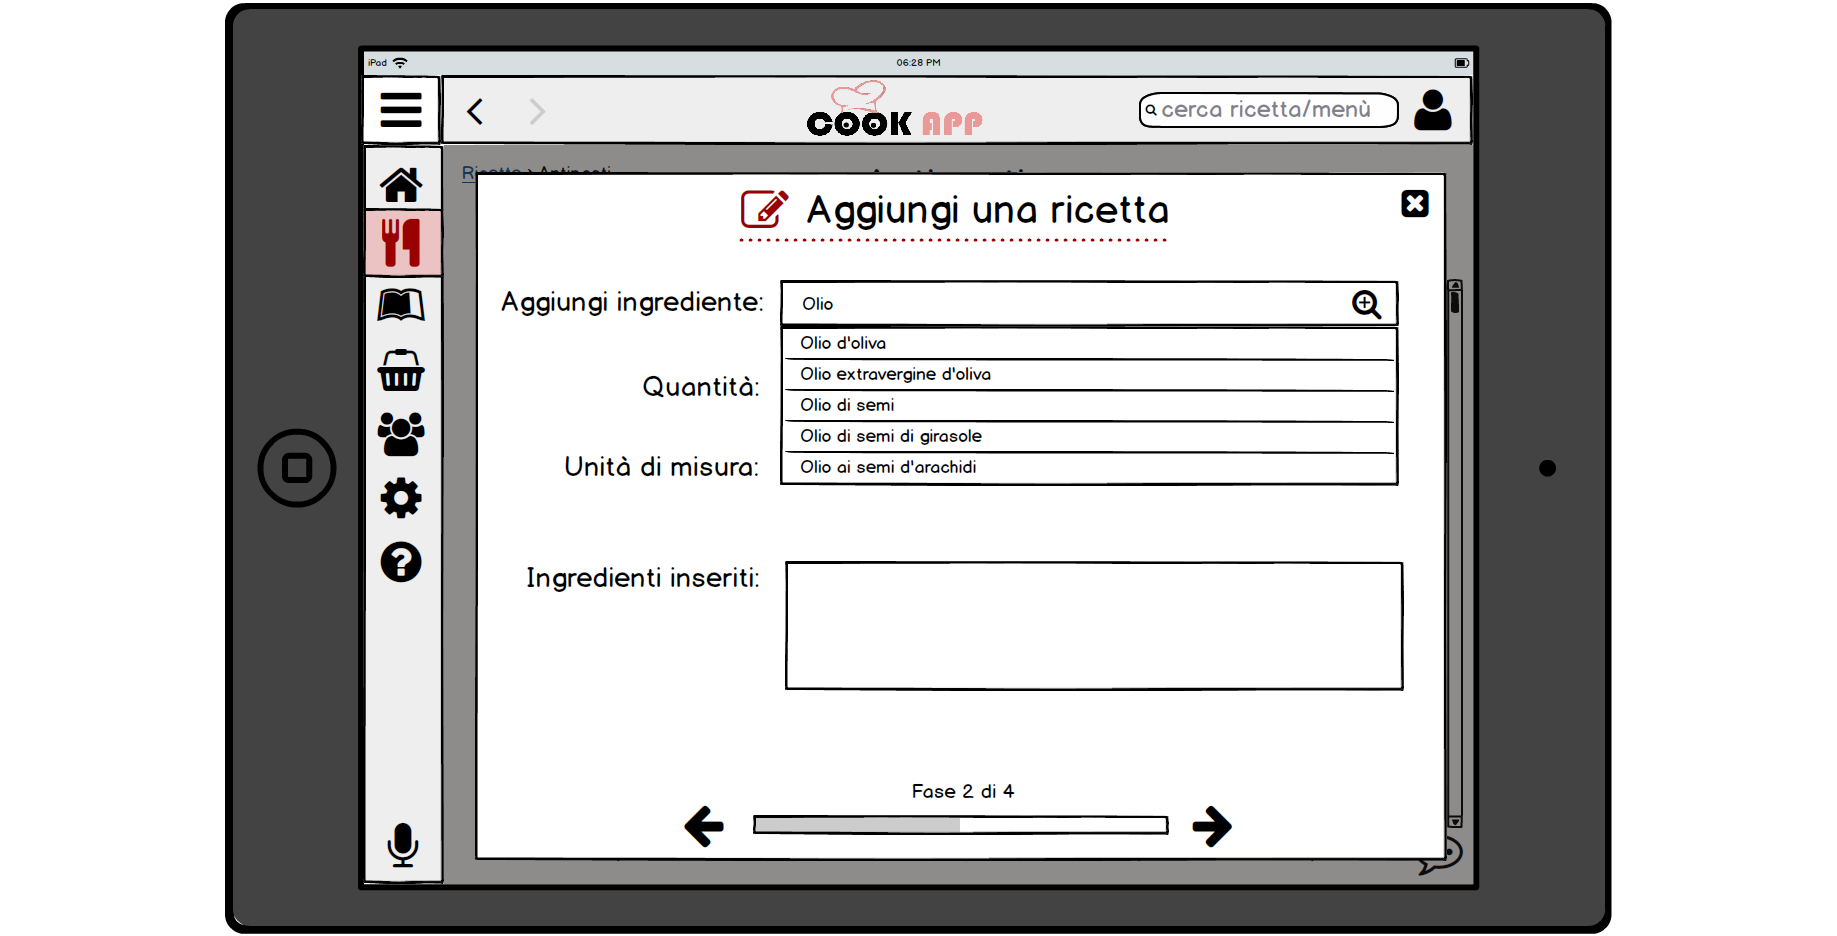
\includegraphics[width=0.95\linewidth]{img/mockup/Aggiungi-ricetta.png}
\end{figure}
\begin{figure}[H]
	\centering
	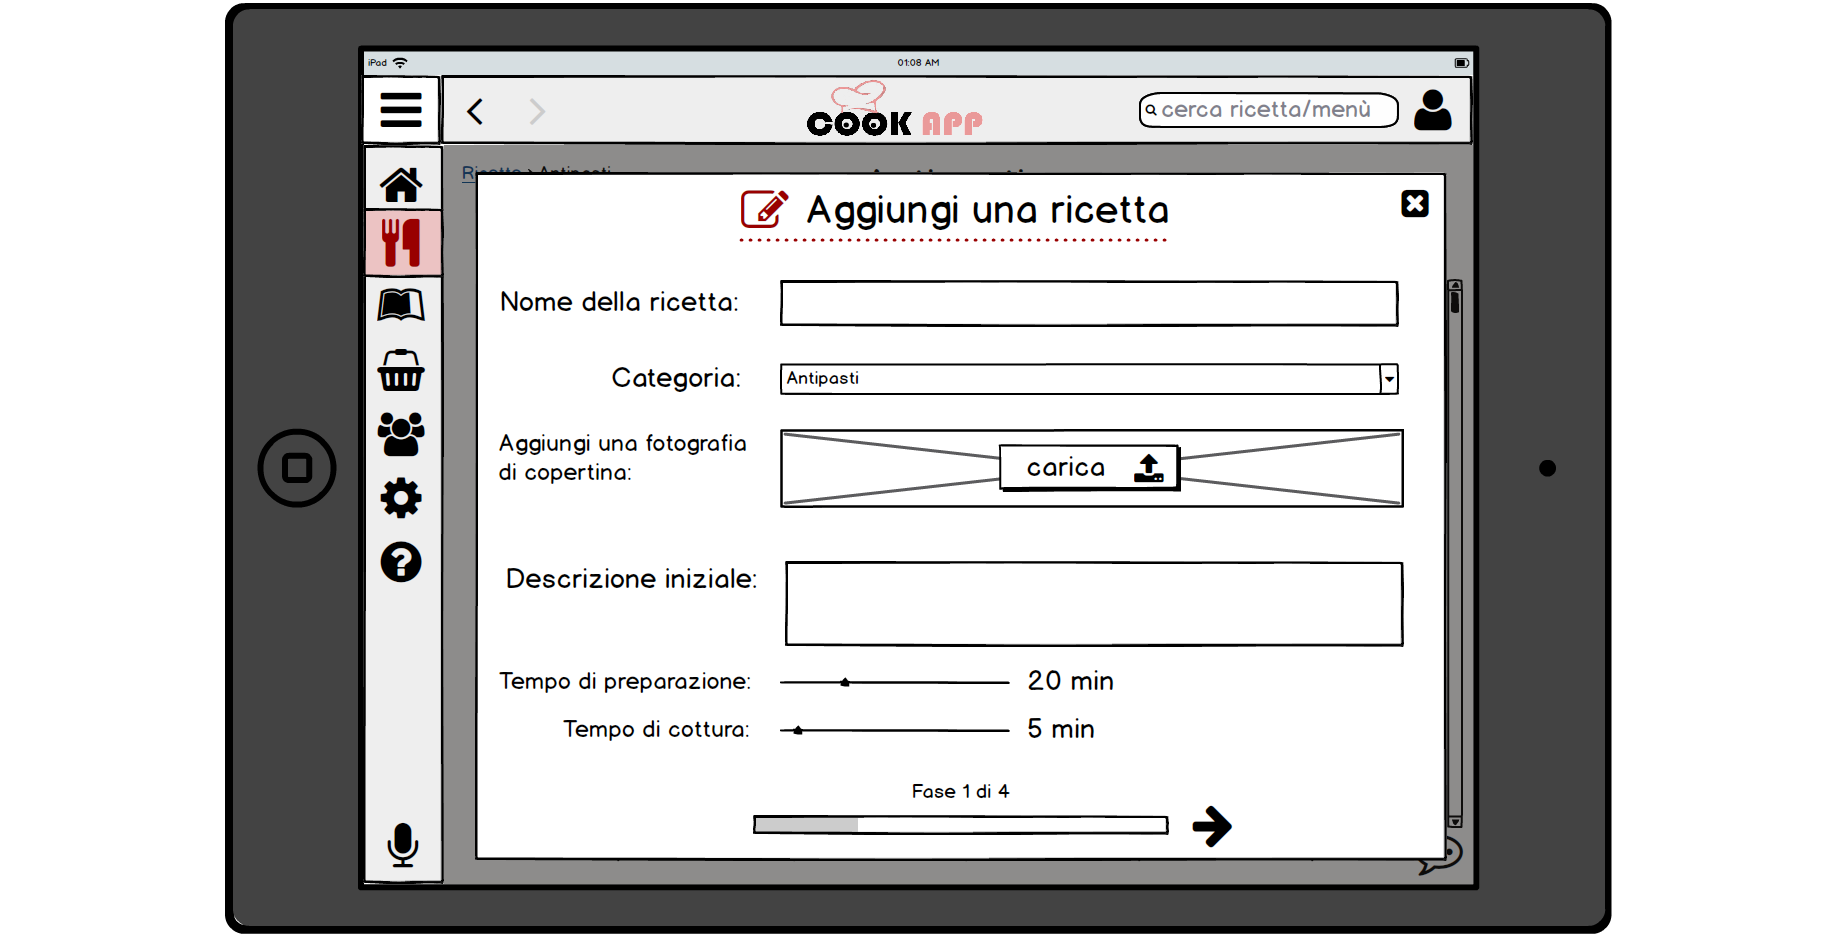
\includegraphics[width=0.95\linewidth]{img/mockup/Aggiungi-ricetta1.png}
\end{figure}
\begin{figure}[H]
	\centering
	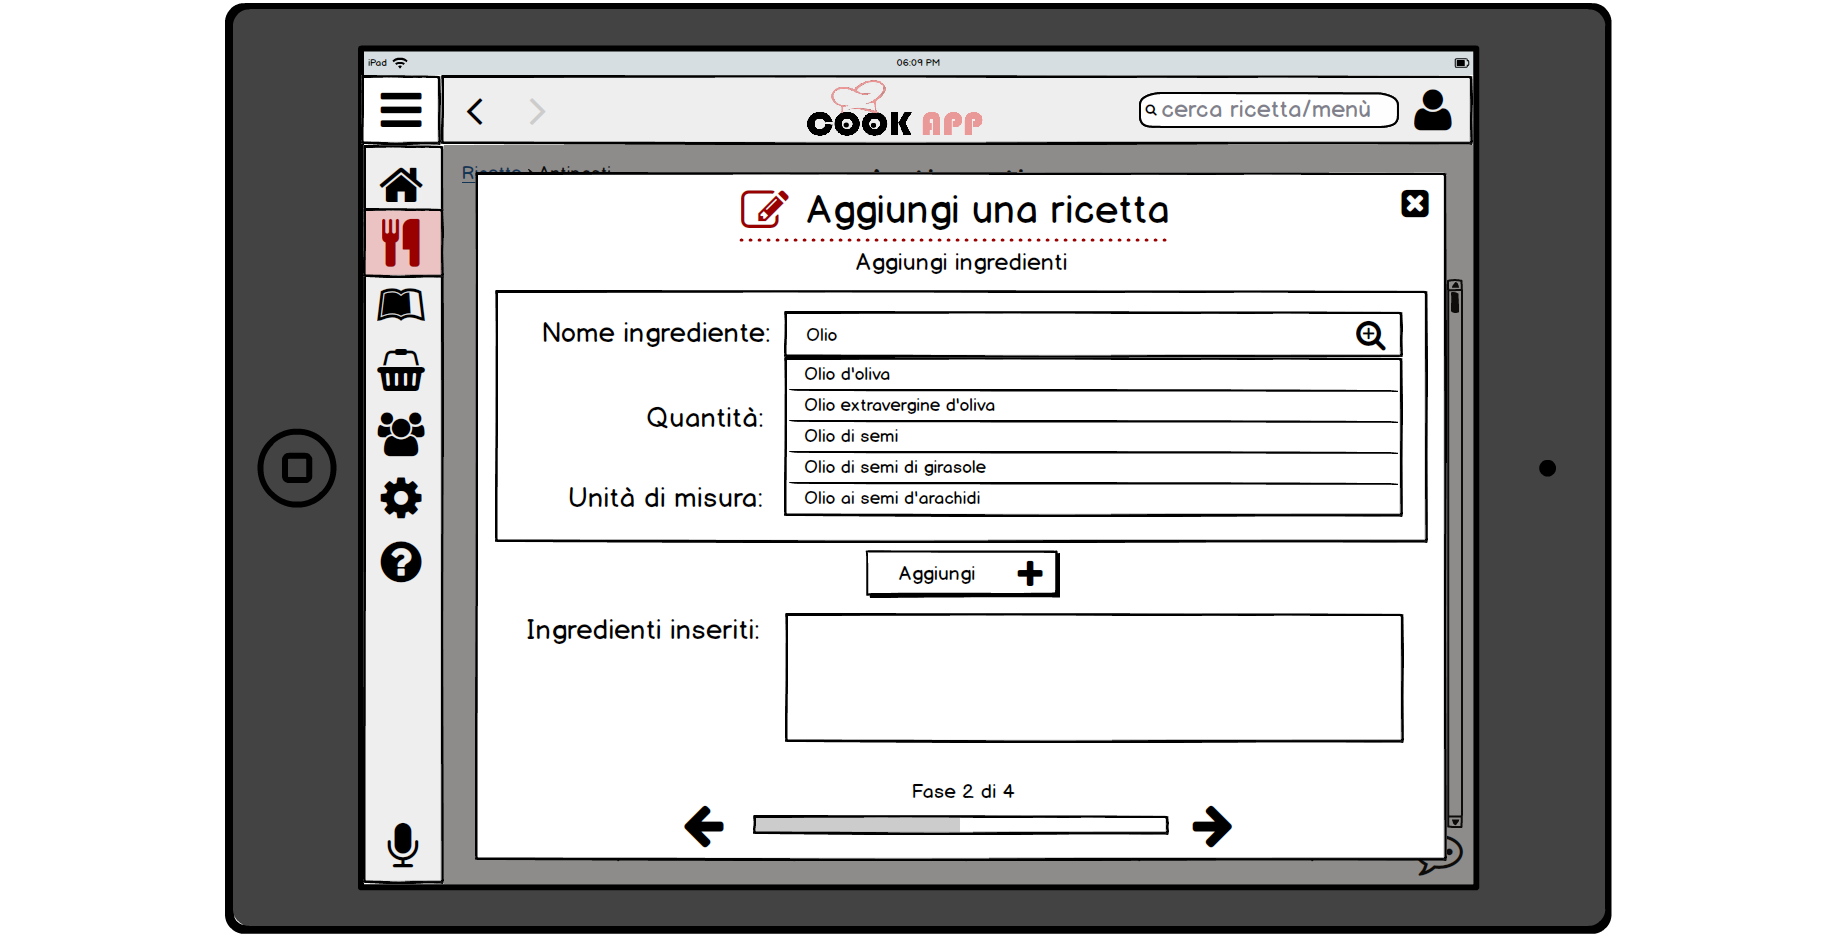
\includegraphics[width=0.95\linewidth]{img/mockup/Aggiungi-ricetta2.png}
\end{figure}
\begin{figure}[H]
	\centering
	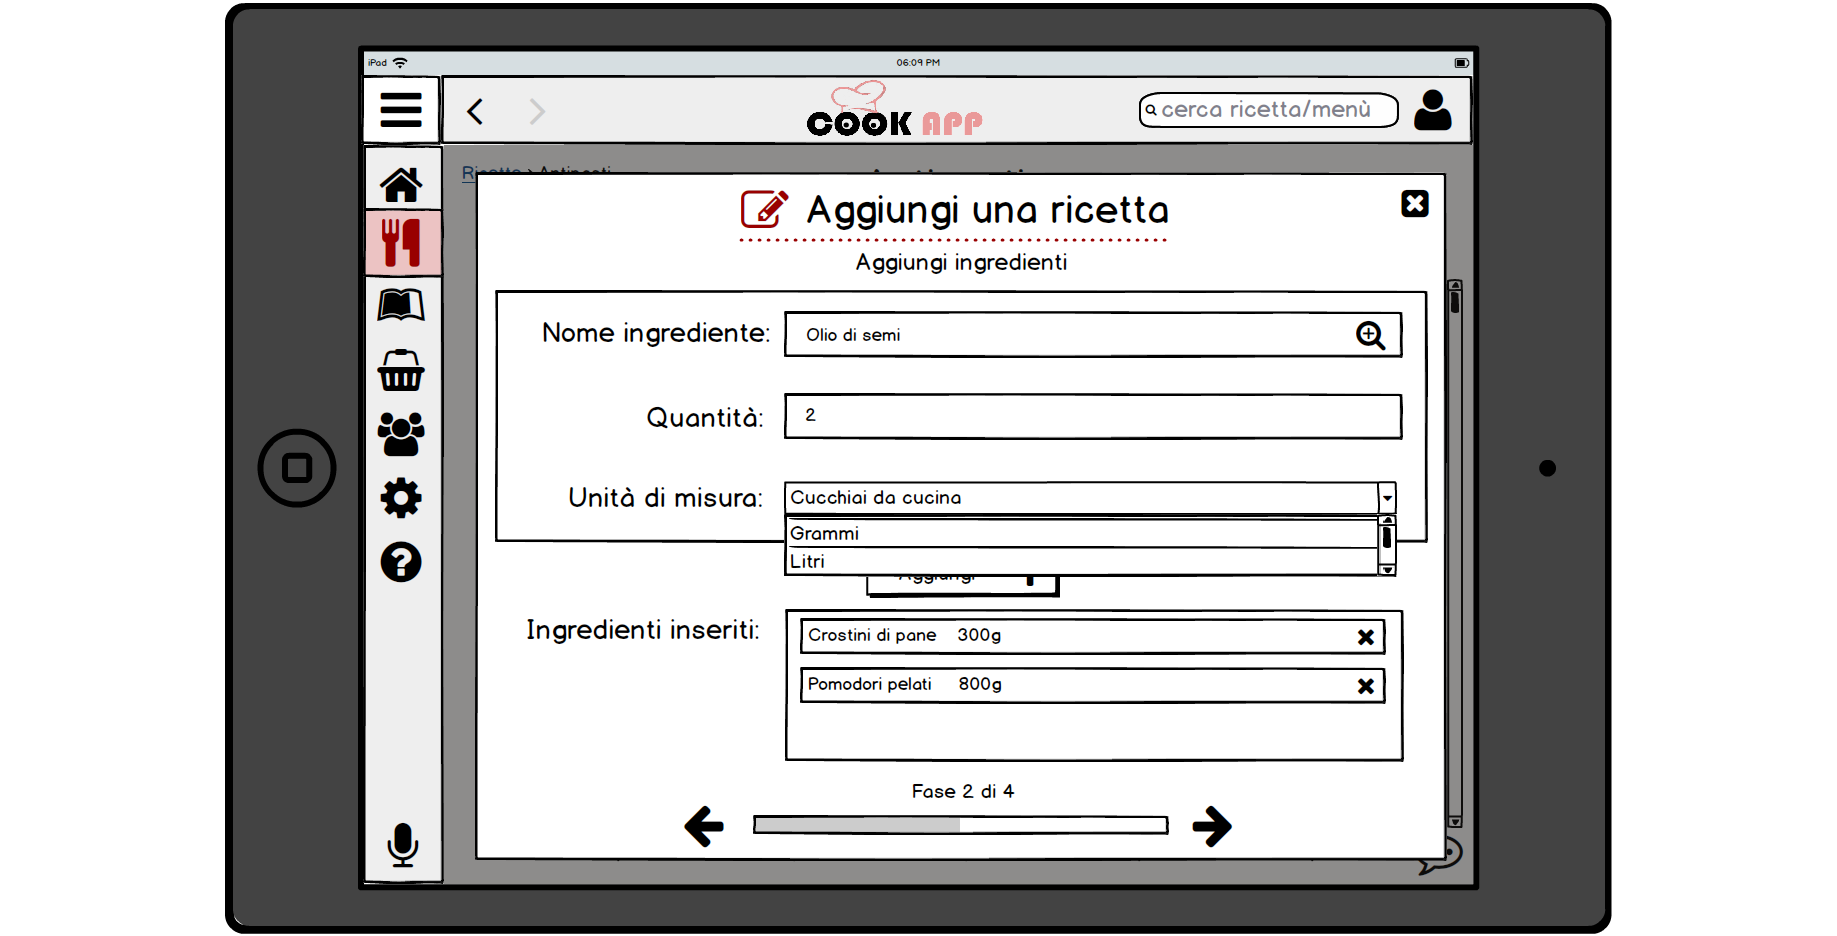
\includegraphics[width=0.95\linewidth]{img/mockup/Aggiungi-ricetta3.png}
\end{figure}
\begin{figure}[H]
	\centering
	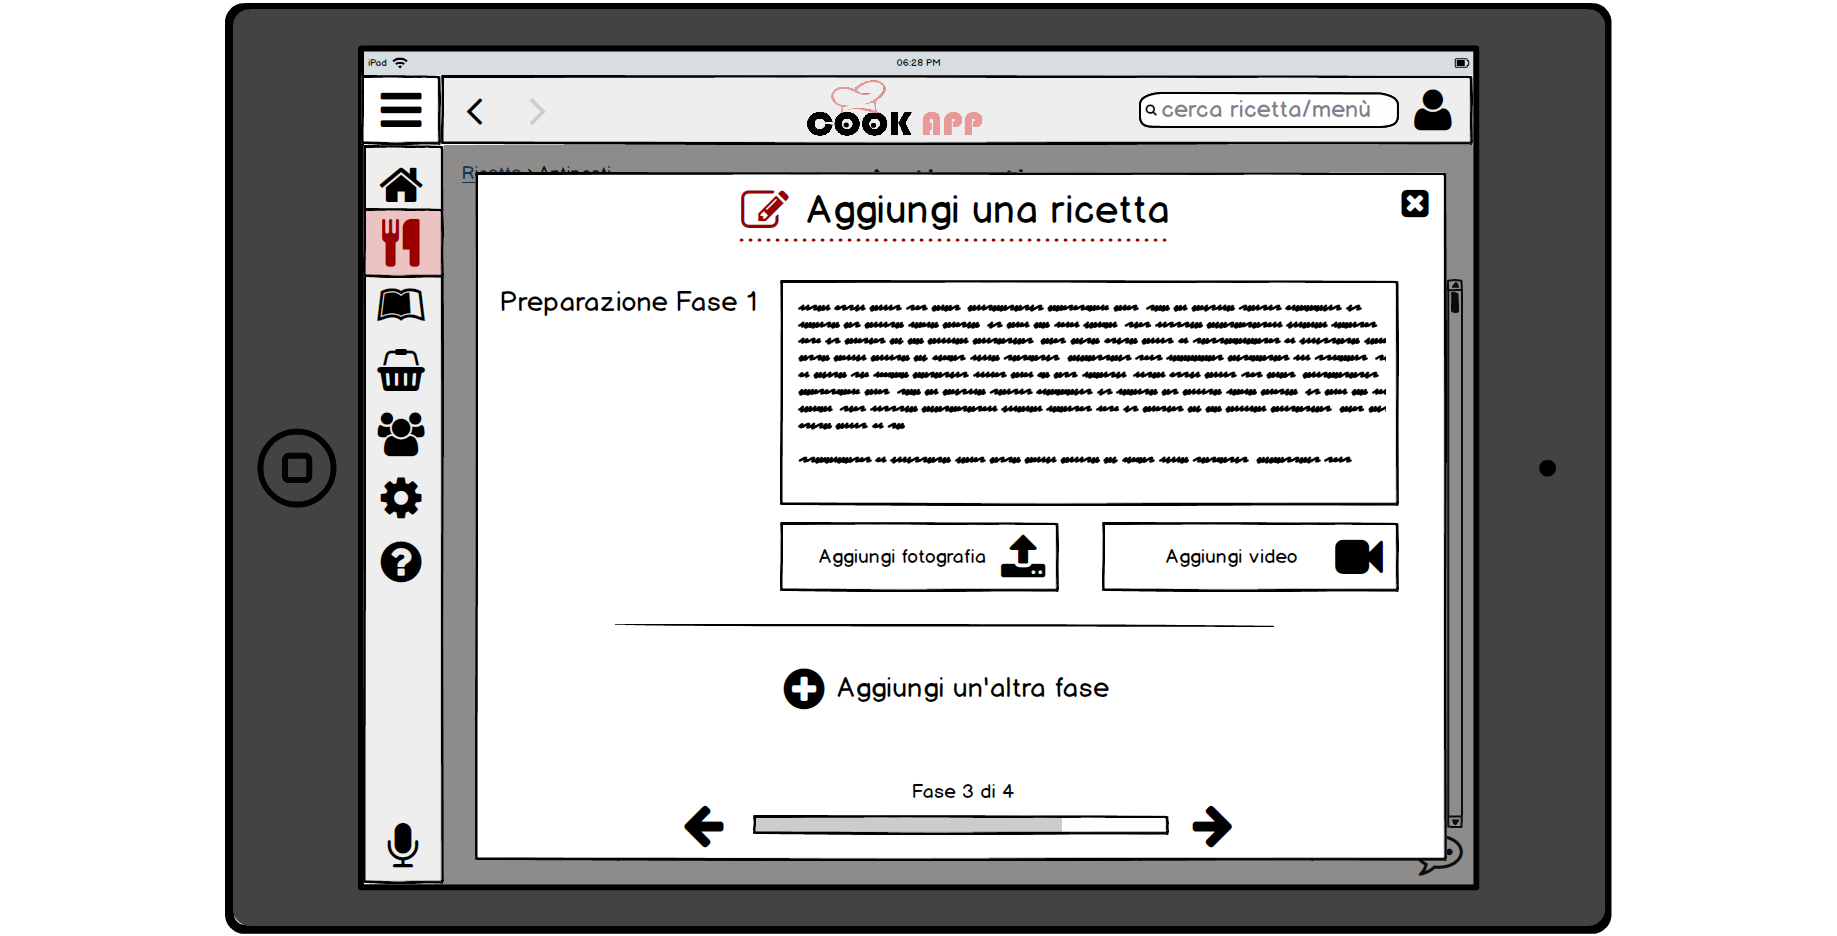
\includegraphics[width=0.95\linewidth]{img/mockup/Aggiungi-ricetta4.png}
\end{figure}
\begin{figure}[H]
	\centering
	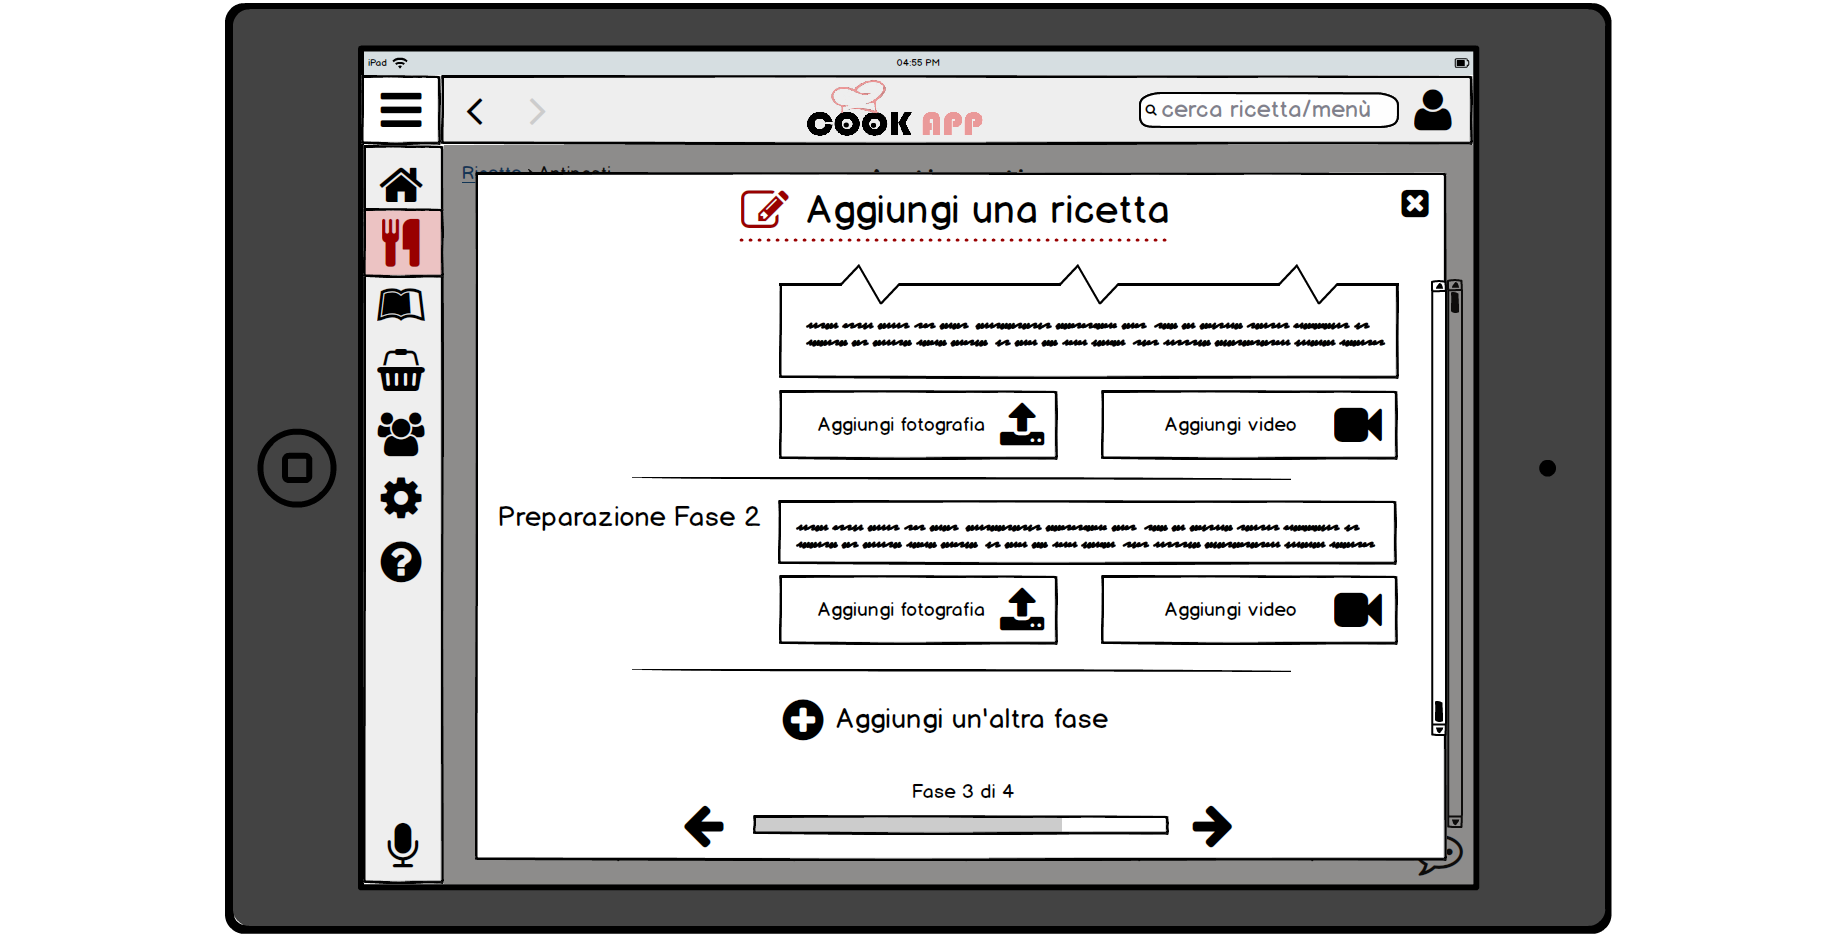
\includegraphics[width=0.95\linewidth]{img/mockup/Aggiungi-ricetta5.png}
\end{figure}
\begin{figure}[H]
	\centering
	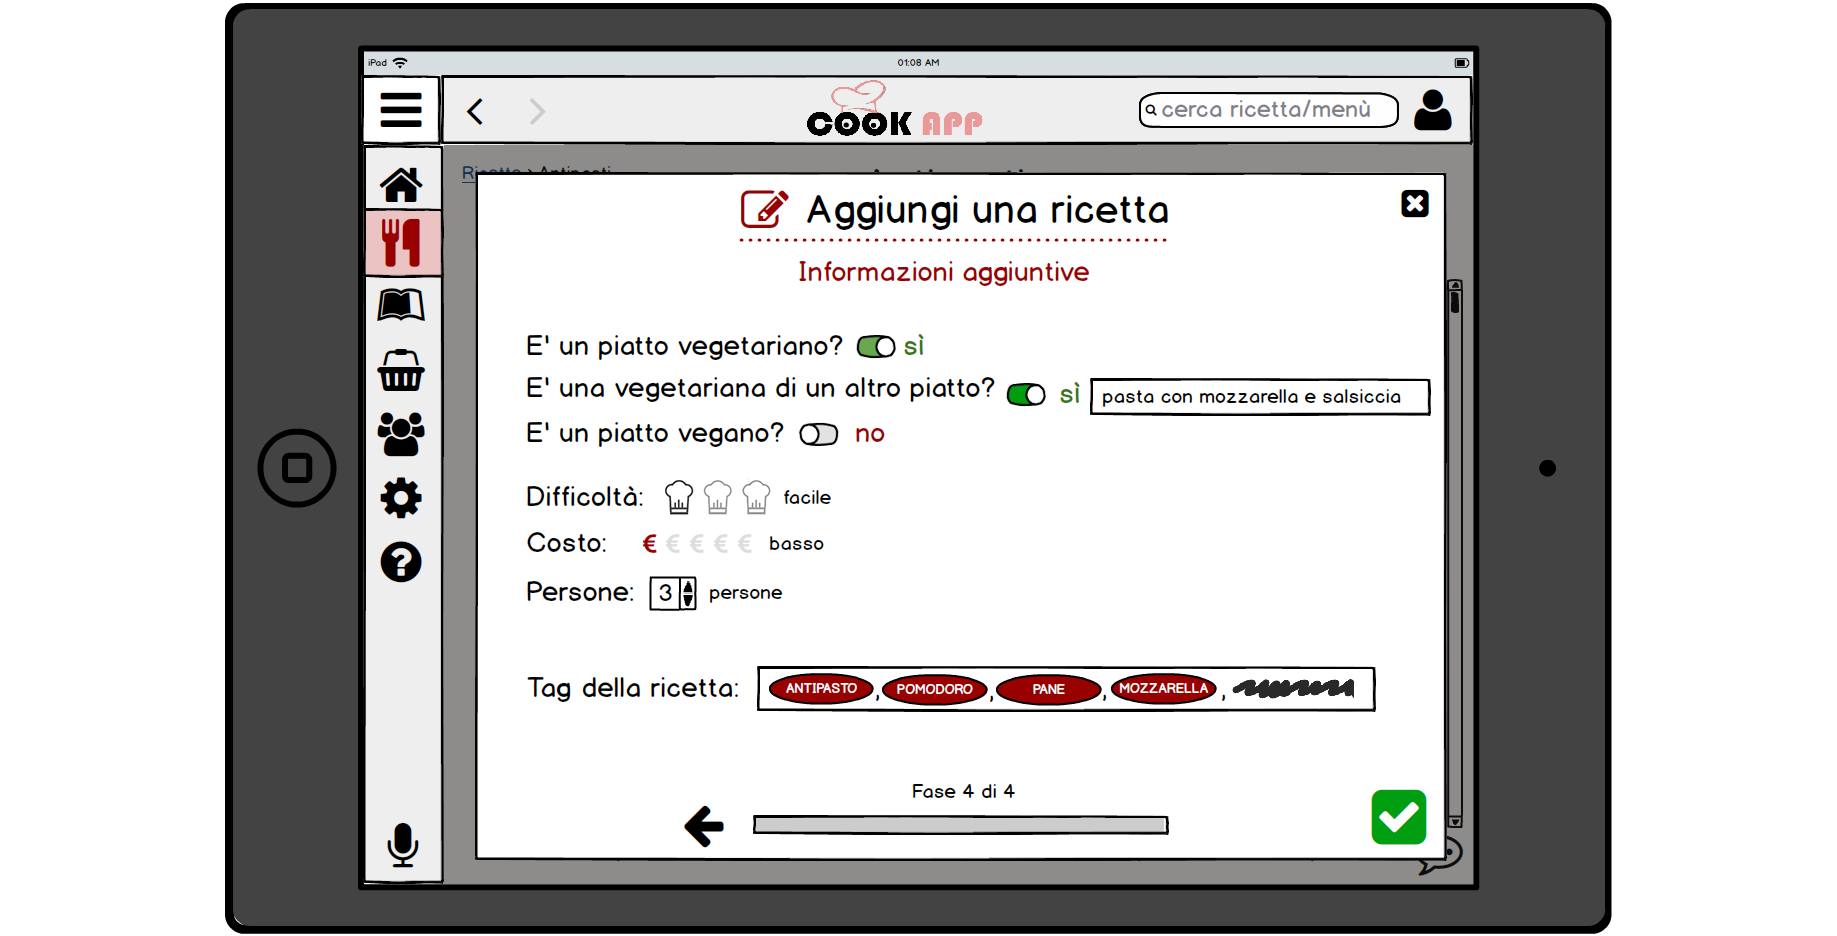
\includegraphics[width=0.95\linewidth]{img/mockup/Aggiungi-ricetta6.png}
\end{figure}
\begin{figure}[H]
	\centering
	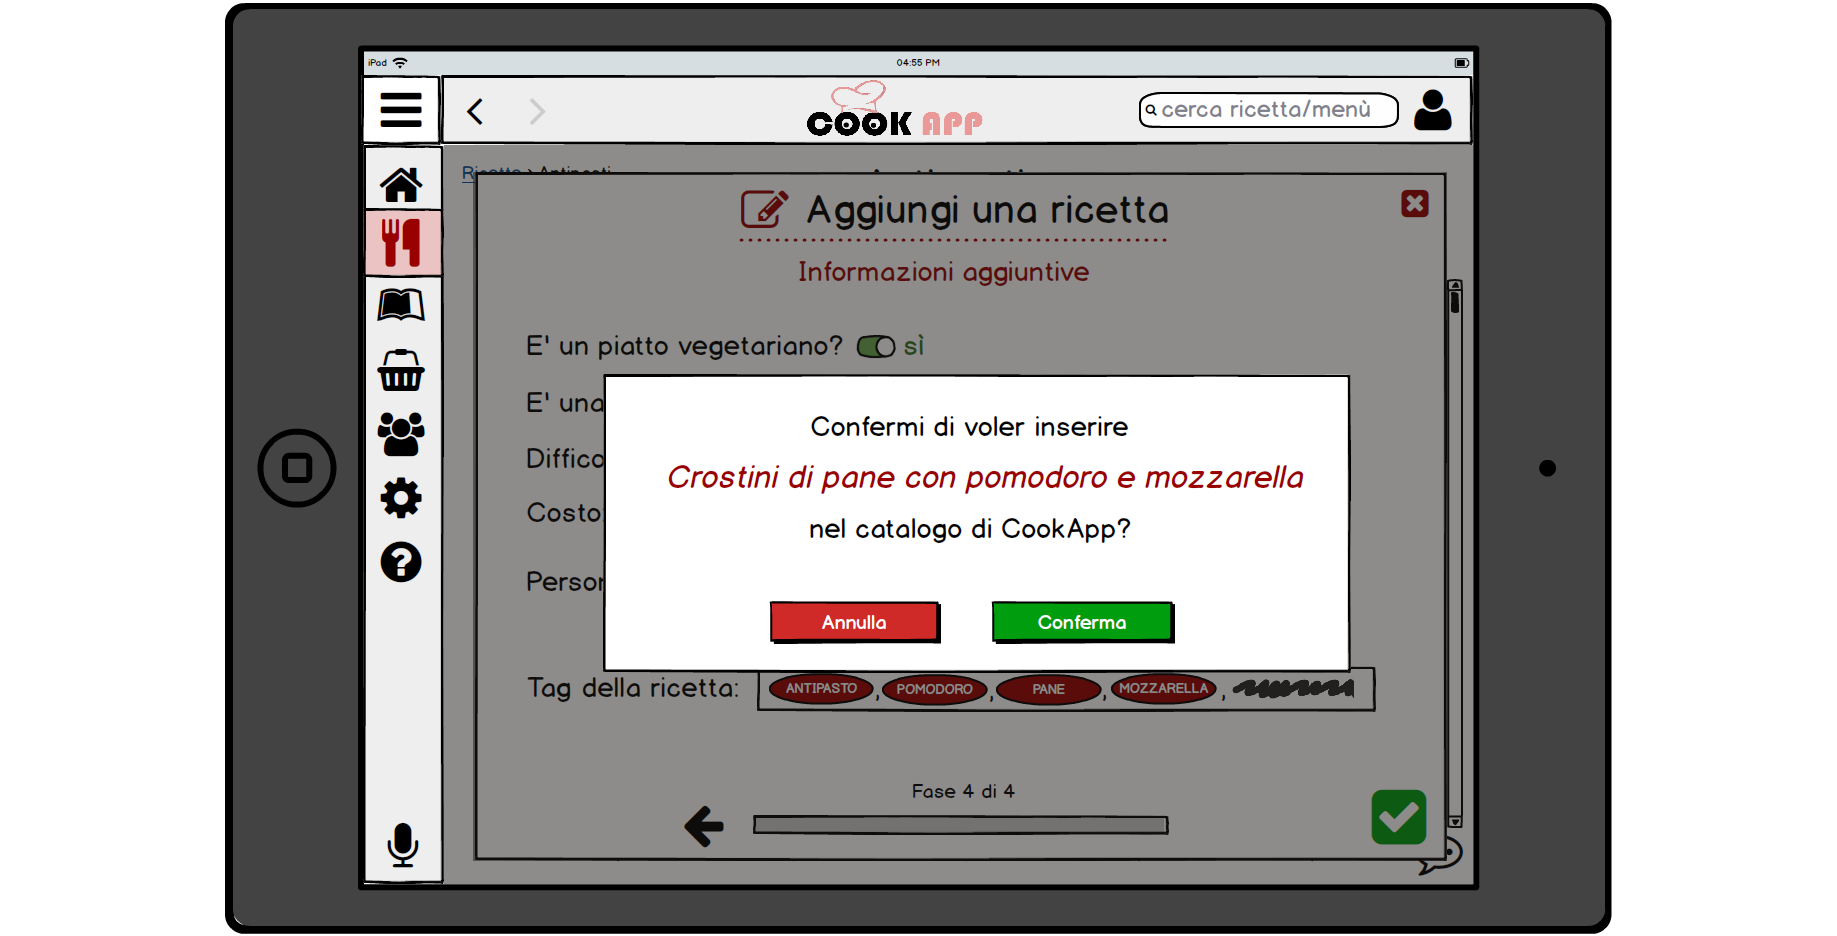
\includegraphics[width=0.95\linewidth]{img/mockup/Aggiungi-ricetta7.png}
\end{figure}
\begin{figure}[H]
	\centering
	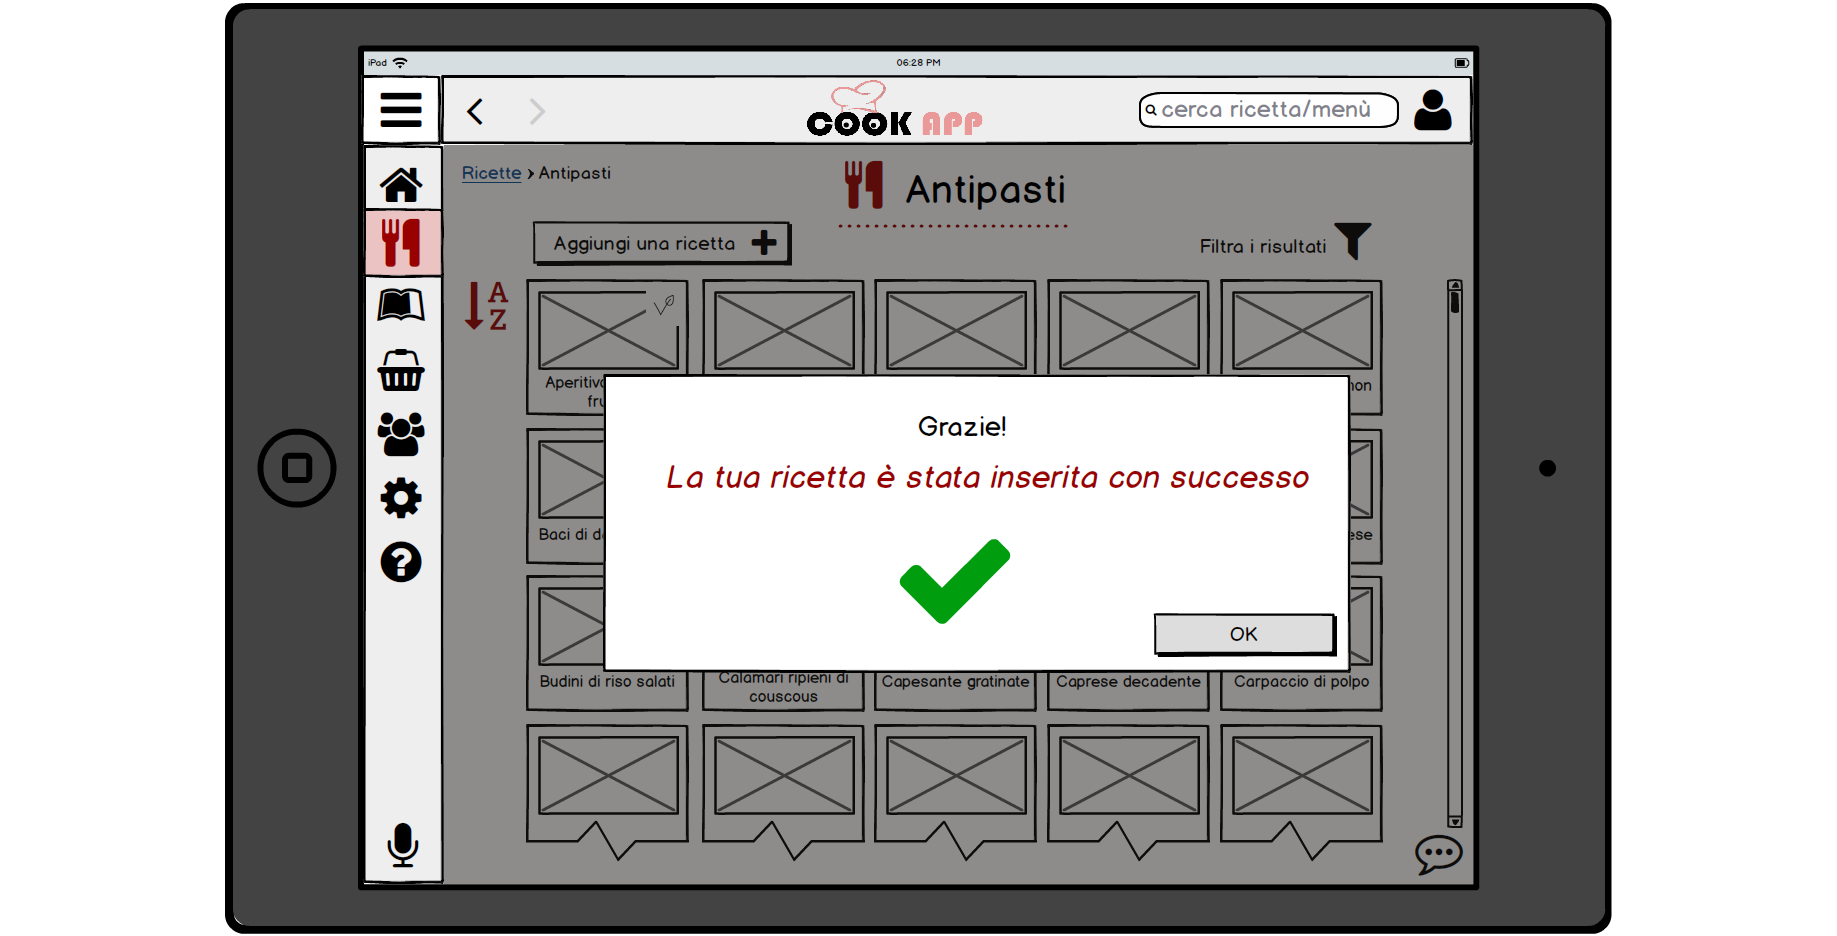
\includegraphics[width=0.95\linewidth]{img/mockup/Aggiungi-ricetta8.png}
\end{figure}
\begin{figure}[H]
	\centering
	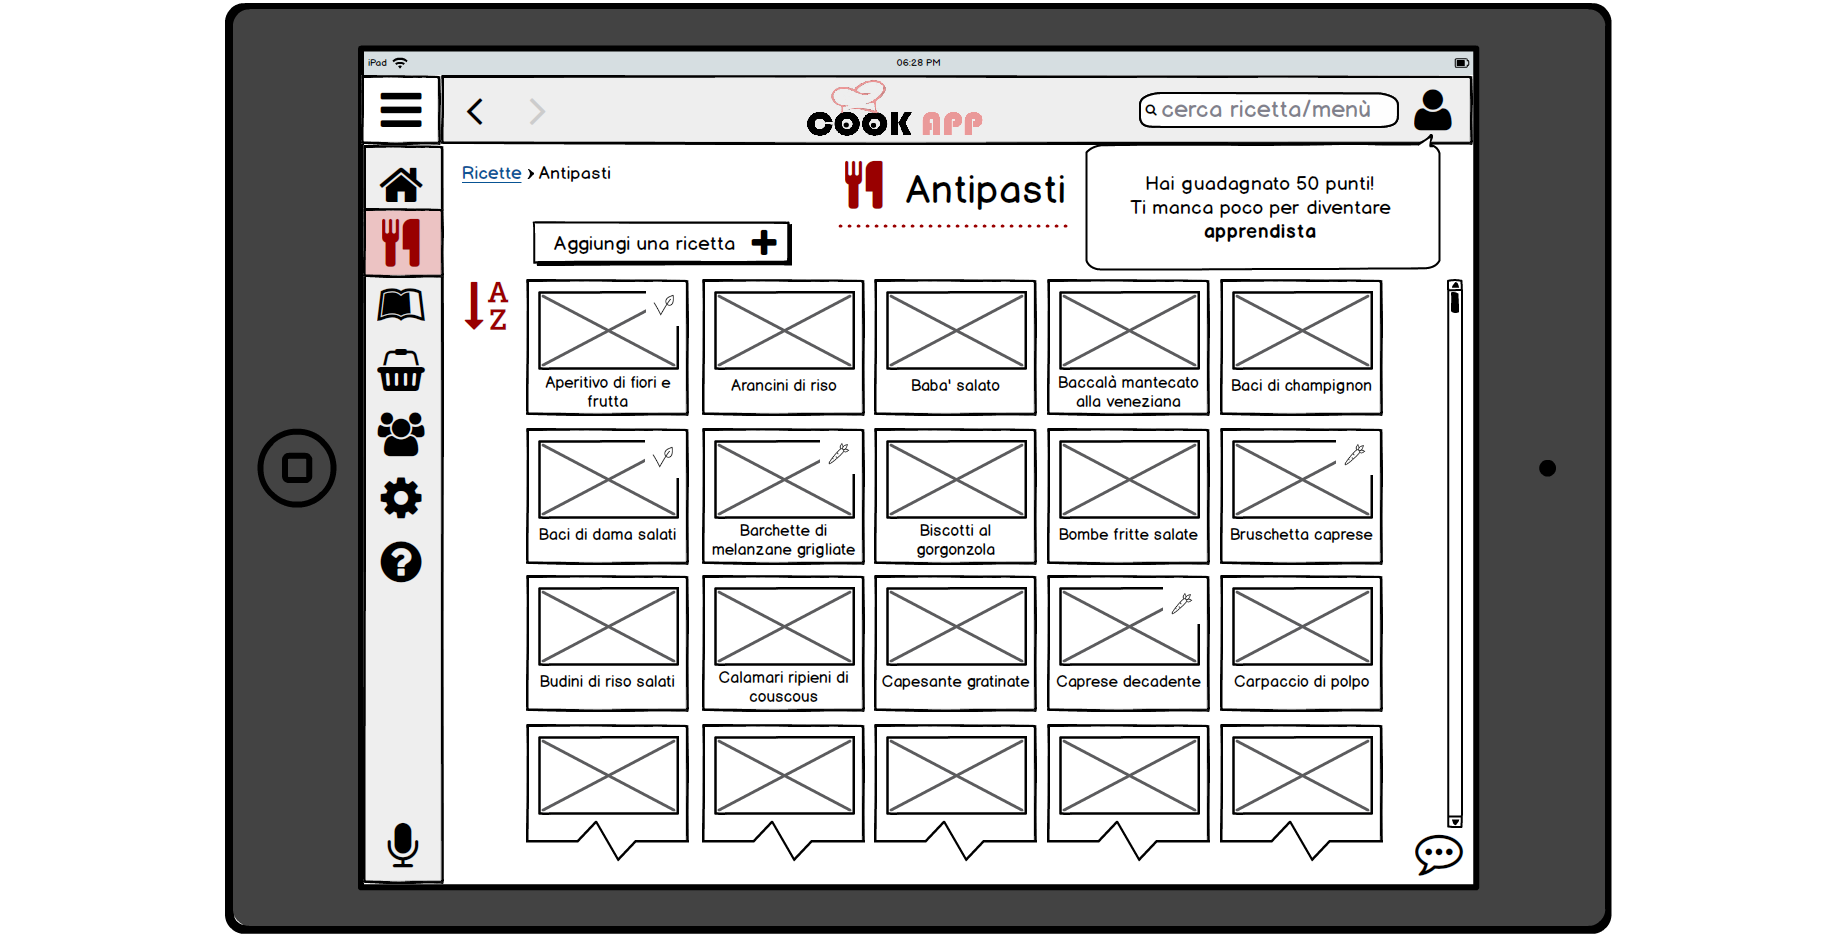
\includegraphics[width=0.95\linewidth]{img/mockup/Aggiungi-ricetta9.png}
\end{figure}


\subsubsection{Catalogo menù}
Il catalogo dei menù offre, in una maniera molto simile al ricettario,
una lista di menù da preparare divisa per categorie. Le categorie sono
diverse: dai menù delle feste, ai pic-nic, ai buffet di diverse
tipologie. La disposizione delle categorie è anche qui organizzata a
mosaico, tramite la quale CookApp da maggiore rilevanza alle catogorie
più votate dalla comunità e selezionate più frequentemente dall'utente.
Dal catologo dei menù, analogalmente al ricettario, è possibile selezionare una categoria di menù,
aggiungere un menù nel catagolo e filtrare i risultati.

\begin{figure}[H]
	\centering
	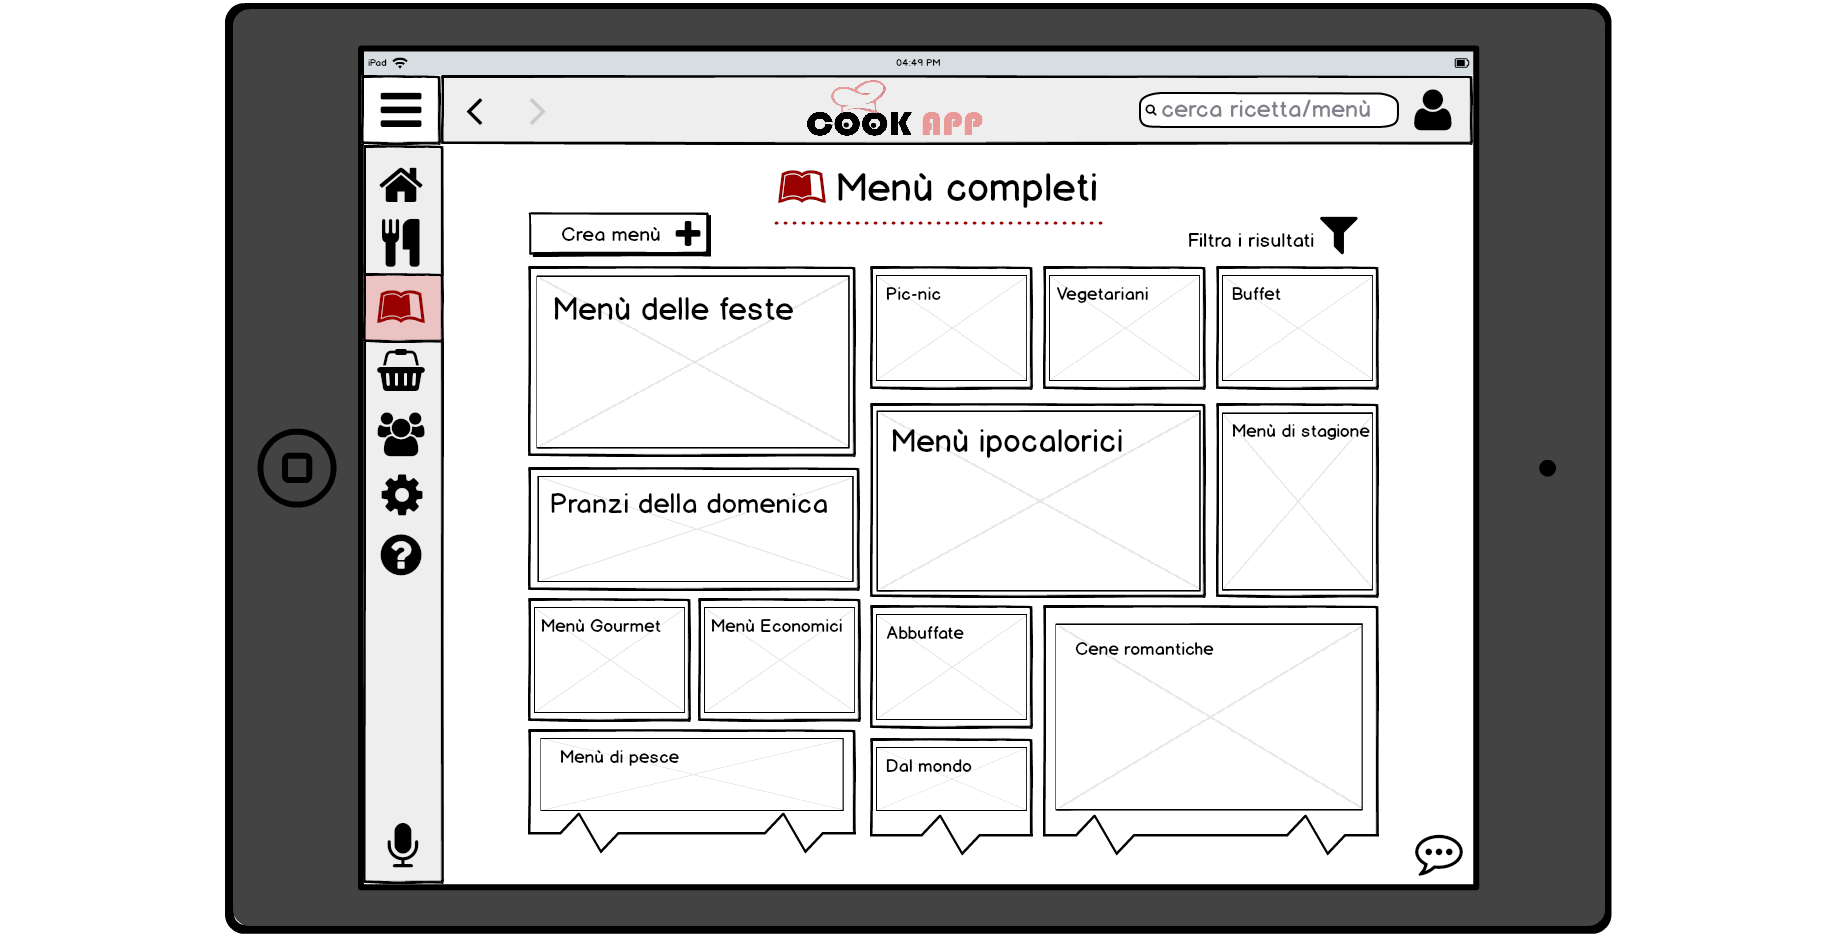
\includegraphics[width=0.95\linewidth]{img/mockup/menu.png}
\end{figure}
\begin{figure}[H]
	\centering
	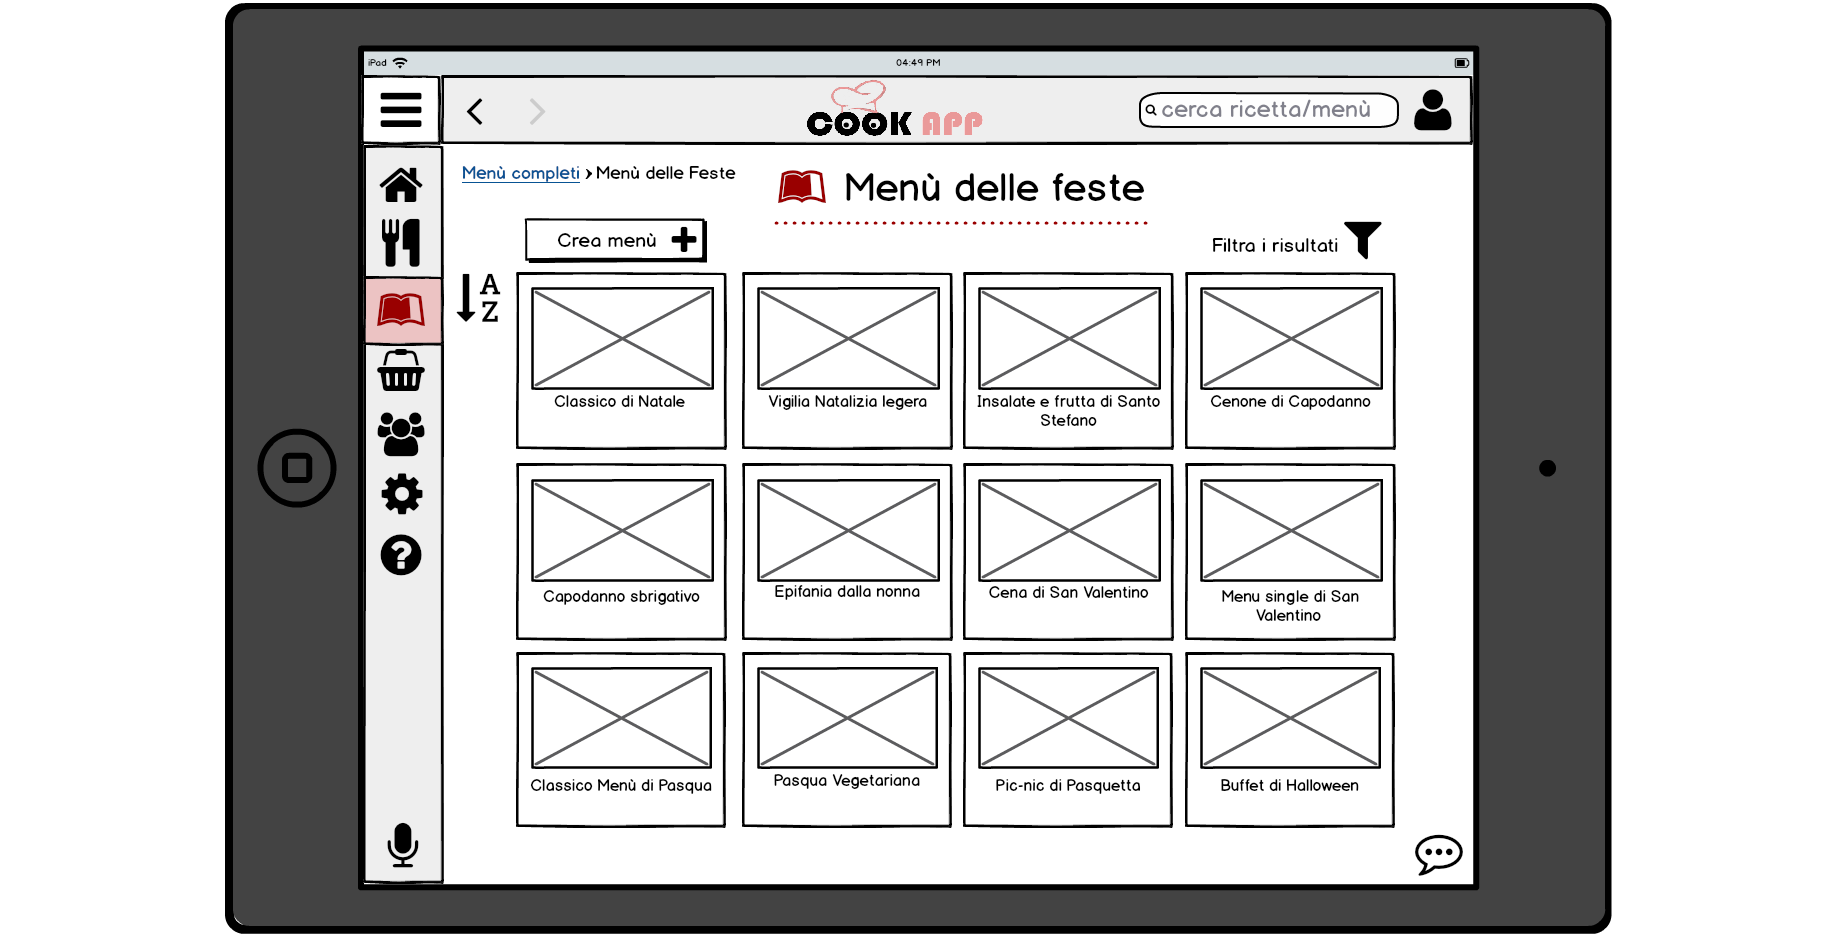
\includegraphics[width=0.95\linewidth]{img/mockup/menu-2.png}
\end{figure}

\subsubsection{Menù}
La schermata di visualizzazione di un menù riprende quella della
visualizzazione di una ricetta.\\ 
Il banner iniziale mostra la fotografia di copertina della menù scelta
dall'utente, insieme alla votazione media delle recensioni e alla
possibilità di eliminare il menù dal catalogo se si è l'autore.\\
Il numero di persone, tempo di preparazione totatle, difficoltà di
realizzazione, costo delle materie prime e numero di persone che hanno
aggiunto la ricetta ai preferiti, sono ben visibili affianco alla
galleria di fotografie della ricette del menù. L'utente ha anche la
possibilità di cambiare il numero di persone del menù. Alla mdifica del
numero di persone del menù, vengono aggiornati i valori del numero di
persone di tutte le ricette del menù e di conseguenza le quantità degli
ingredienti.\\
Scorrendo la schermata, vengono mostrate le ricette che fanno parte del
menù. In fondo alla lista delle ricette c'è un riquadro che permette di
aggiungere/rimuovere un menù ai preferiti, aggiungerne gli ingredienti
alla lista della spesa, personalizzare il menù creandone una copia da 

\begin{figure}[H]
	\centering
	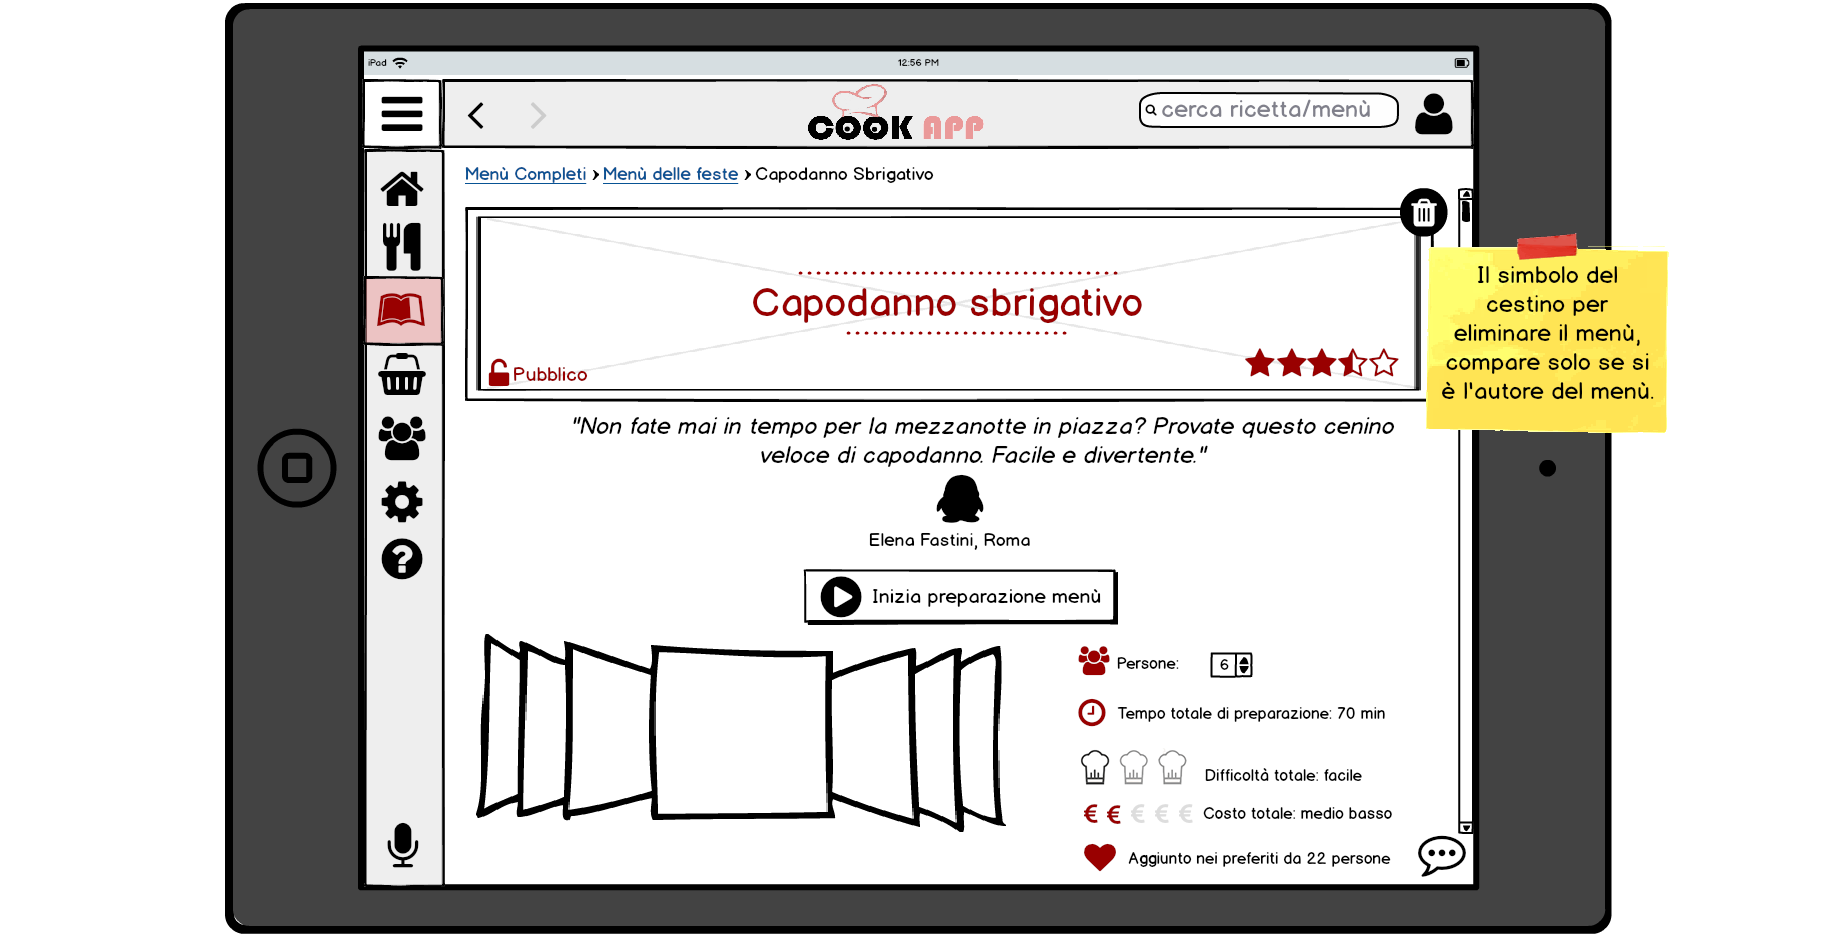
\includegraphics[width=0.95\linewidth]{img/mockup/menu-overview-1.png}
\end{figure}
\begin{figure}[H]
	\centering
	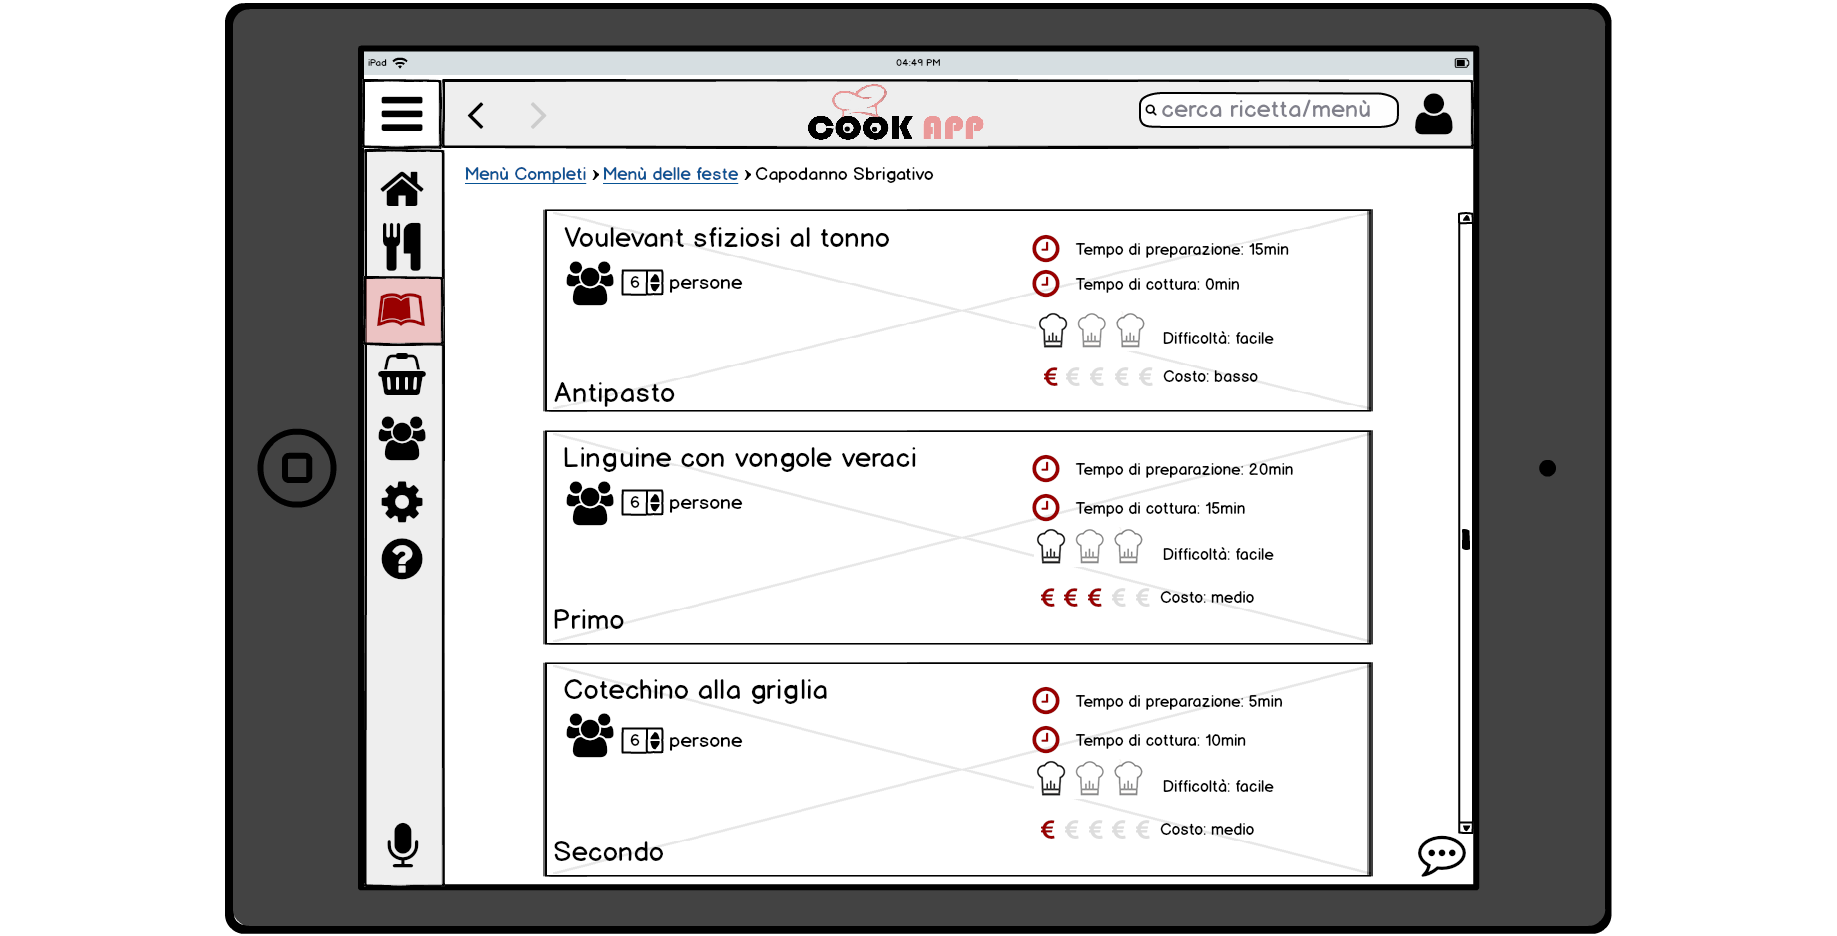
\includegraphics[width=0.95\linewidth]{img/mockup/menu-overview-2.png}
\end{figure}
\begin{figure}[H]
	\centering
	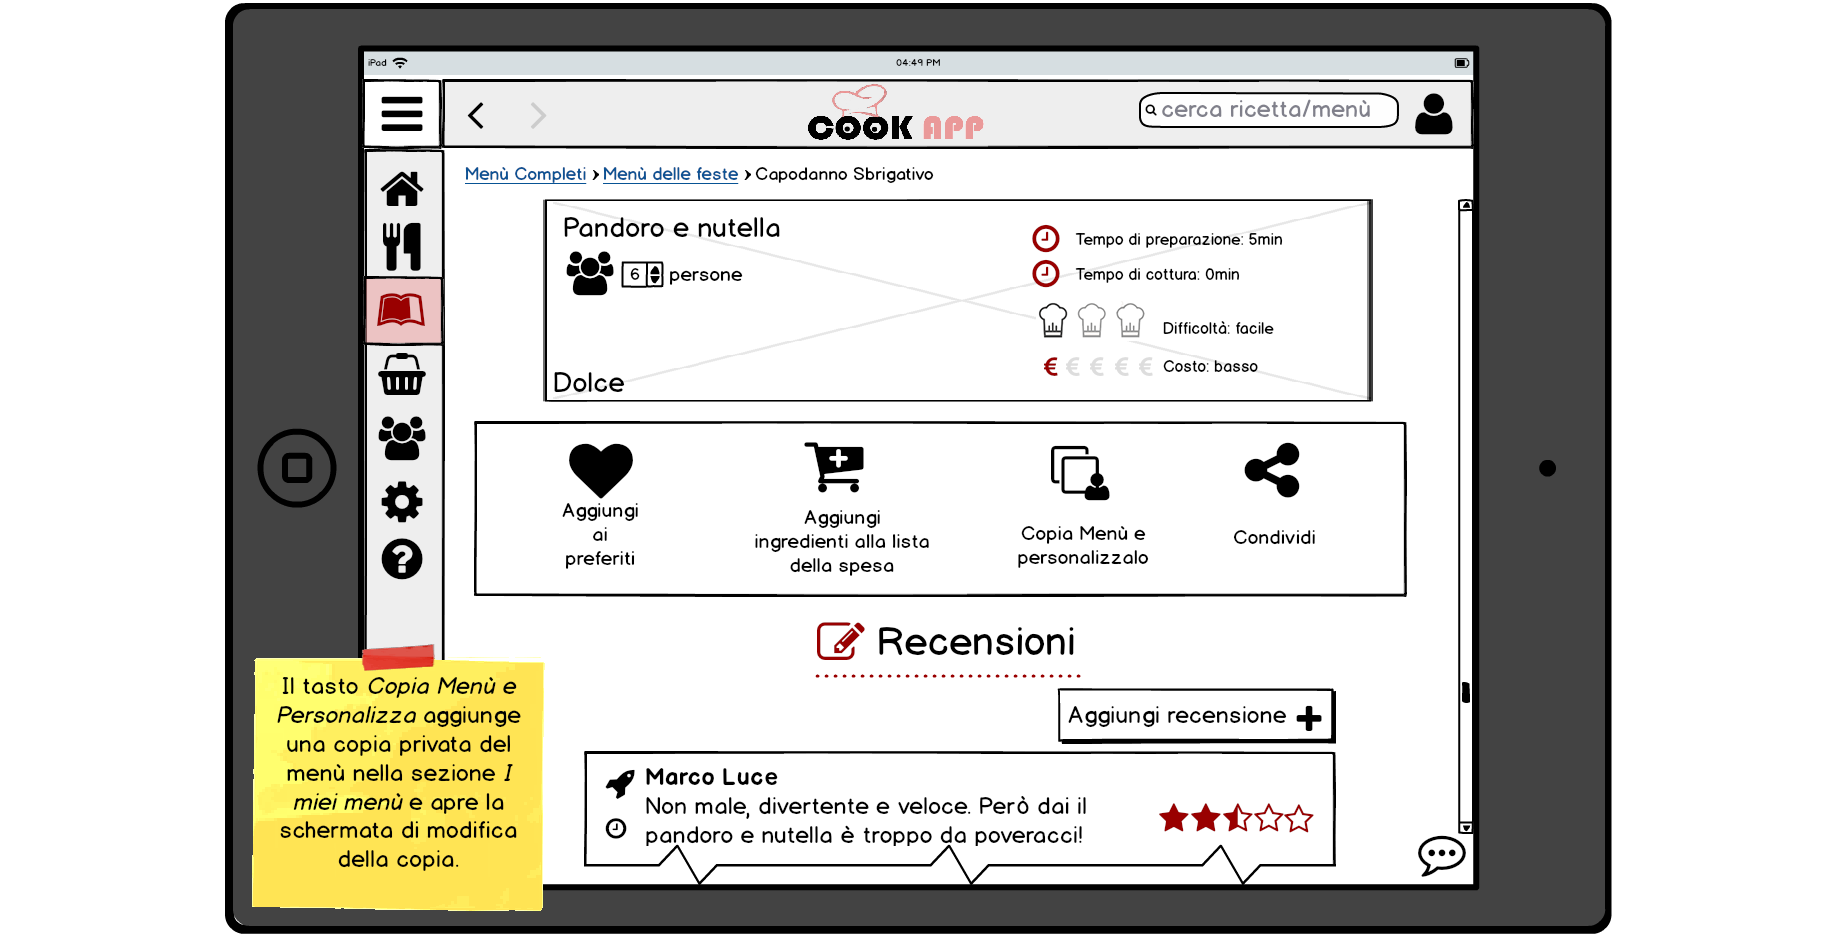
\includegraphics[width=0.95\linewidth]{img/mockup/menu-overview-3.png}
\end{figure}
\begin{figure}[H]
	\centering
	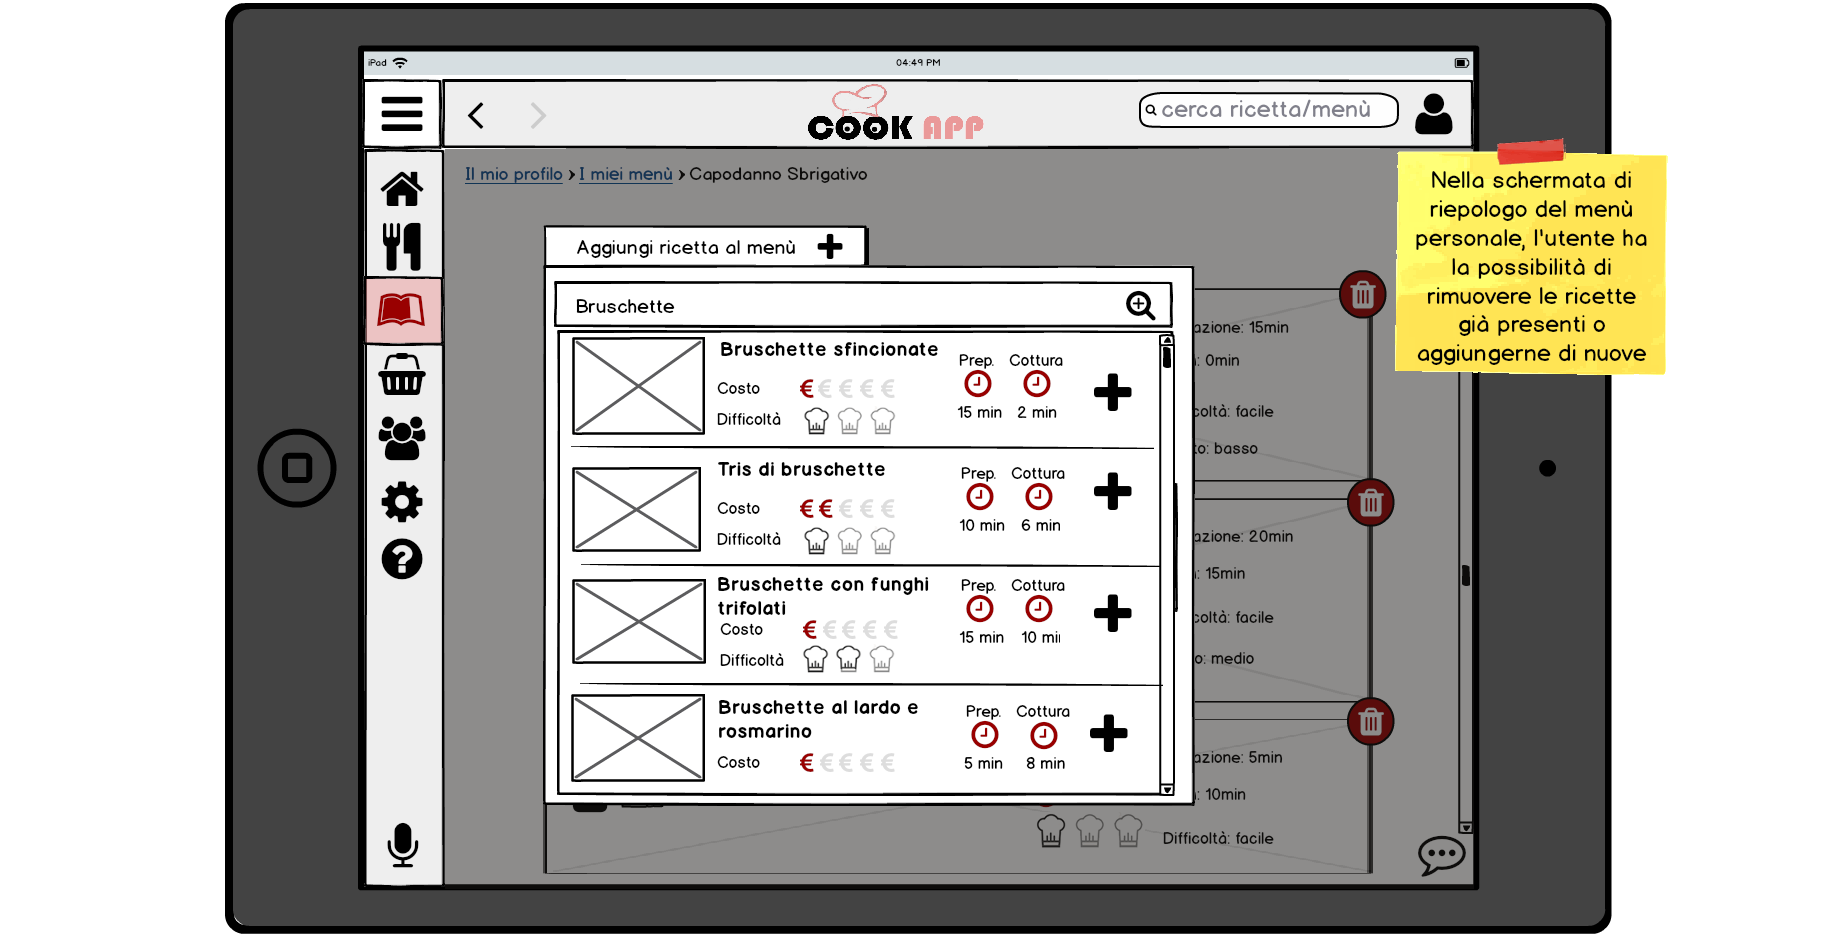
\includegraphics[width=0.95\linewidth]{img/mockup/menu-overview-4.png}
\end{figure}

\subsubsection{Menù preparazione}
TODO

\subsubsection{Menù personale}
\TODO

\subsubsection{Crea menù}
Selezionando il pulsante ``Crea menù'' dalla schermata iniziale del
catalogo dei menù o da una sua categoria, viene aperto un form diviso in
3 fasi che permette di comporre un nuovo menù da un insieme di
ricette.\\
L'utente può scegliere se crearlo ``pubblico'' oppure ``privato''. Nel primo
caso verrà inserito nel catalogo dei menù e sarà visibile da tutti gli
utenti di CookApp, mentre nel secondo caso verrà aggiunto nella sezione
``I miei menù'' all'interno del profilo.\\ 
Il form di creazione è molto simile al form di aggiunta di una ricetta.
Le differenza principale è che in questo caso l'utente può aggiungere
nel menù da creare le ricette già esistenti nel ricettario tramite
l'apposito strumento di ricerca ricette riproposto nel form. Il tempo di
preparazione totale viene calcolato come somma dei tempi di preparazione
delle ricette inserite, ma è comunque modificale dall'utente tramite uno
slider. Il costo, la difficoltà e il numero di persone della fase 3 sono preimpostati
in base alle media dei parametri delle singole ricette inserite, ma
anche in questo caso sono modificabili dall'utente.\\
Una volta terminata la creazione, CookApp assegna 20 punti all'utente
per la creazione di un 
menù privato e 50 per la creazione di un menù pubblico, incentivando
così la creazione di menù da inserire nel catalogo. 

\begin{figure}[H]
	\centering
	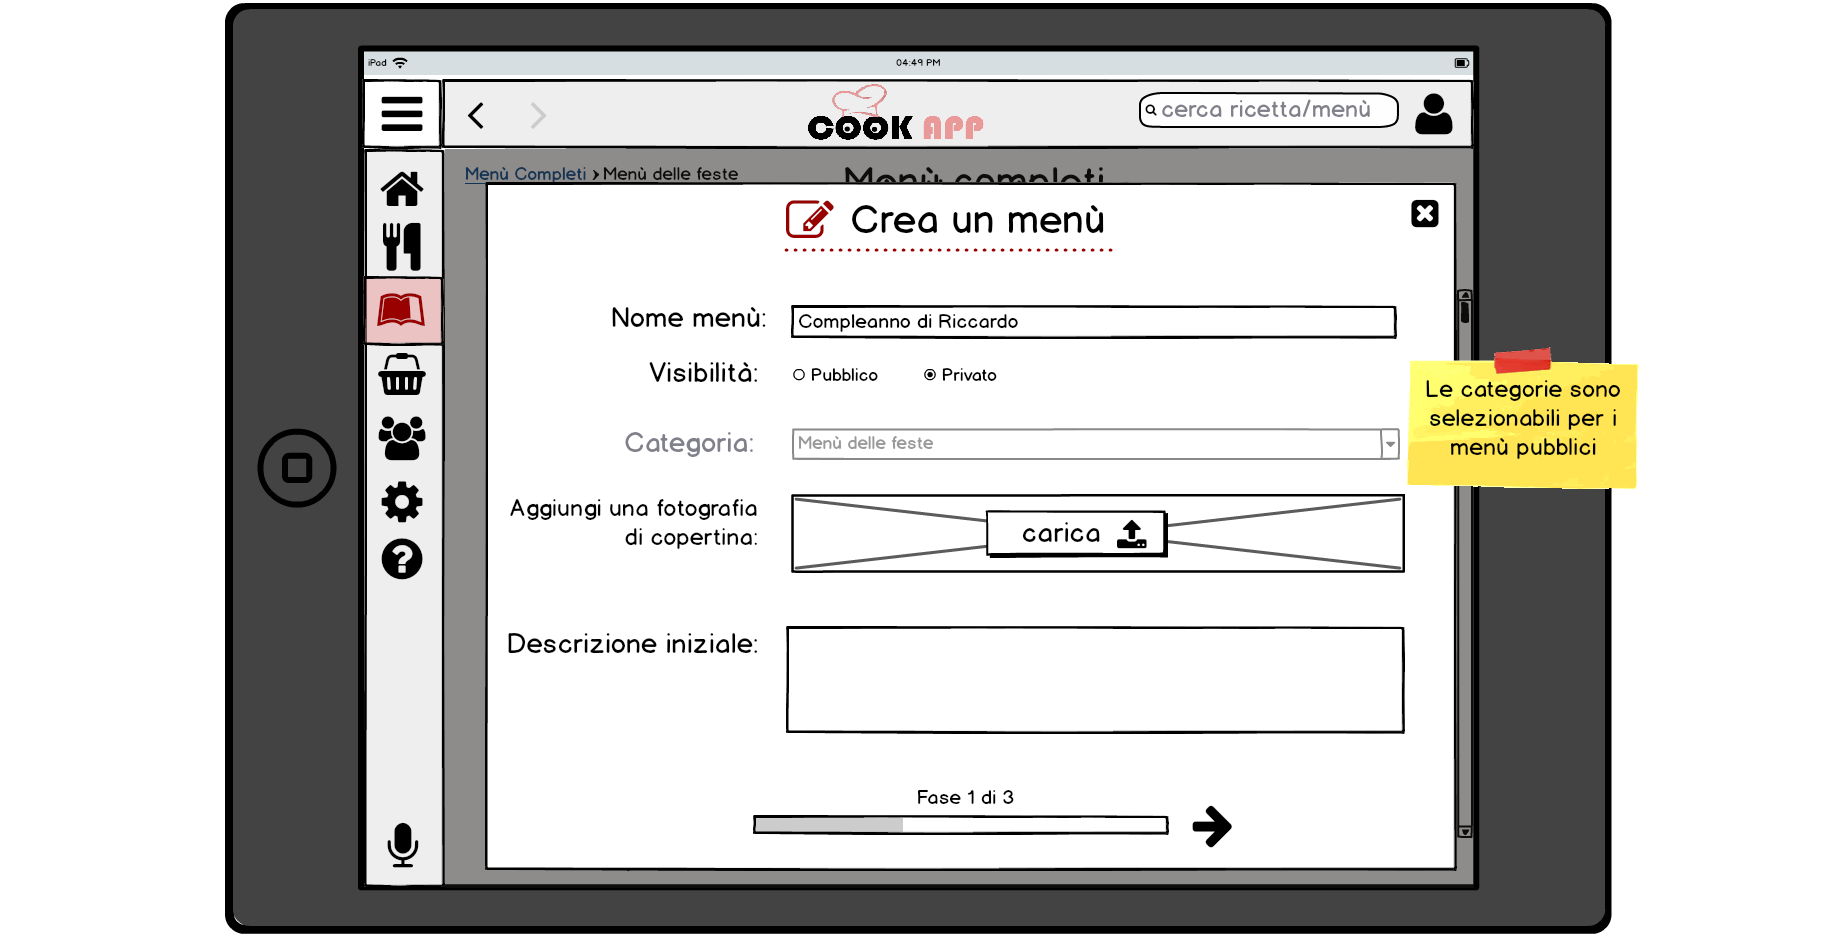
\includegraphics[width=0.95\linewidth]{img/mockup/menu-crea.png}
\end{figure}
\begin{figure}[H]
	\centering
	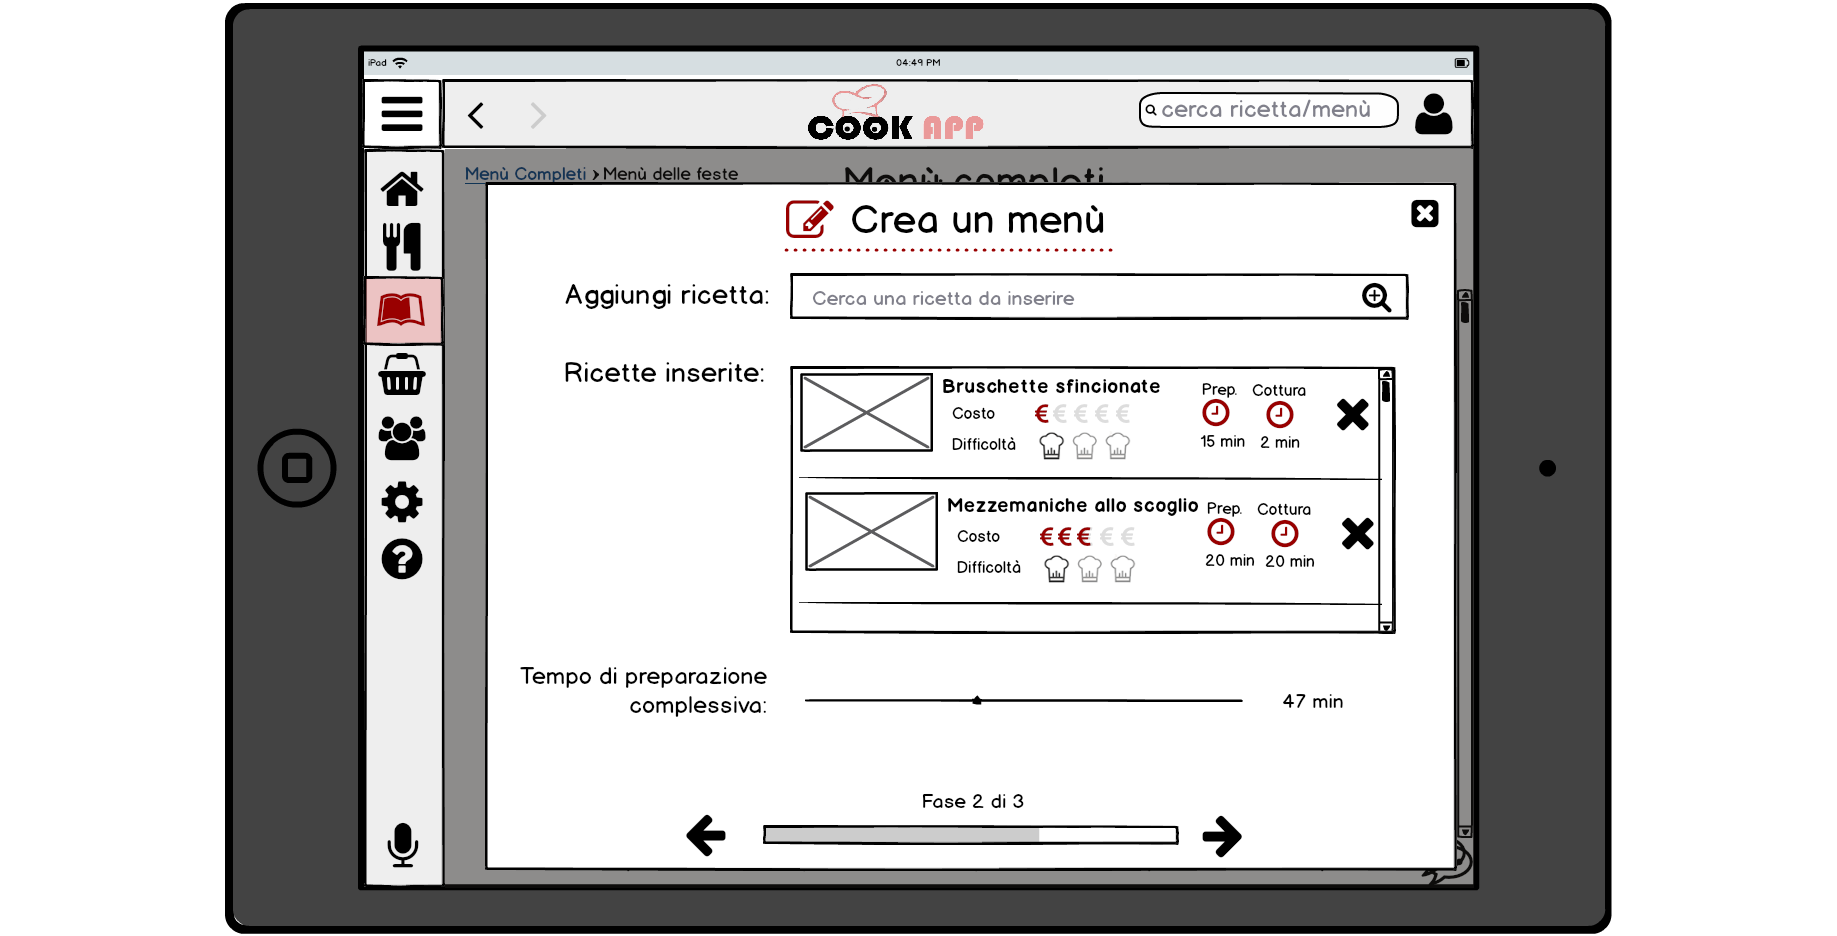
\includegraphics[width=0.95\linewidth]{img/mockup/menu-crea-2.png}
\end{figure}
\begin{figure}[H]
	\centering
	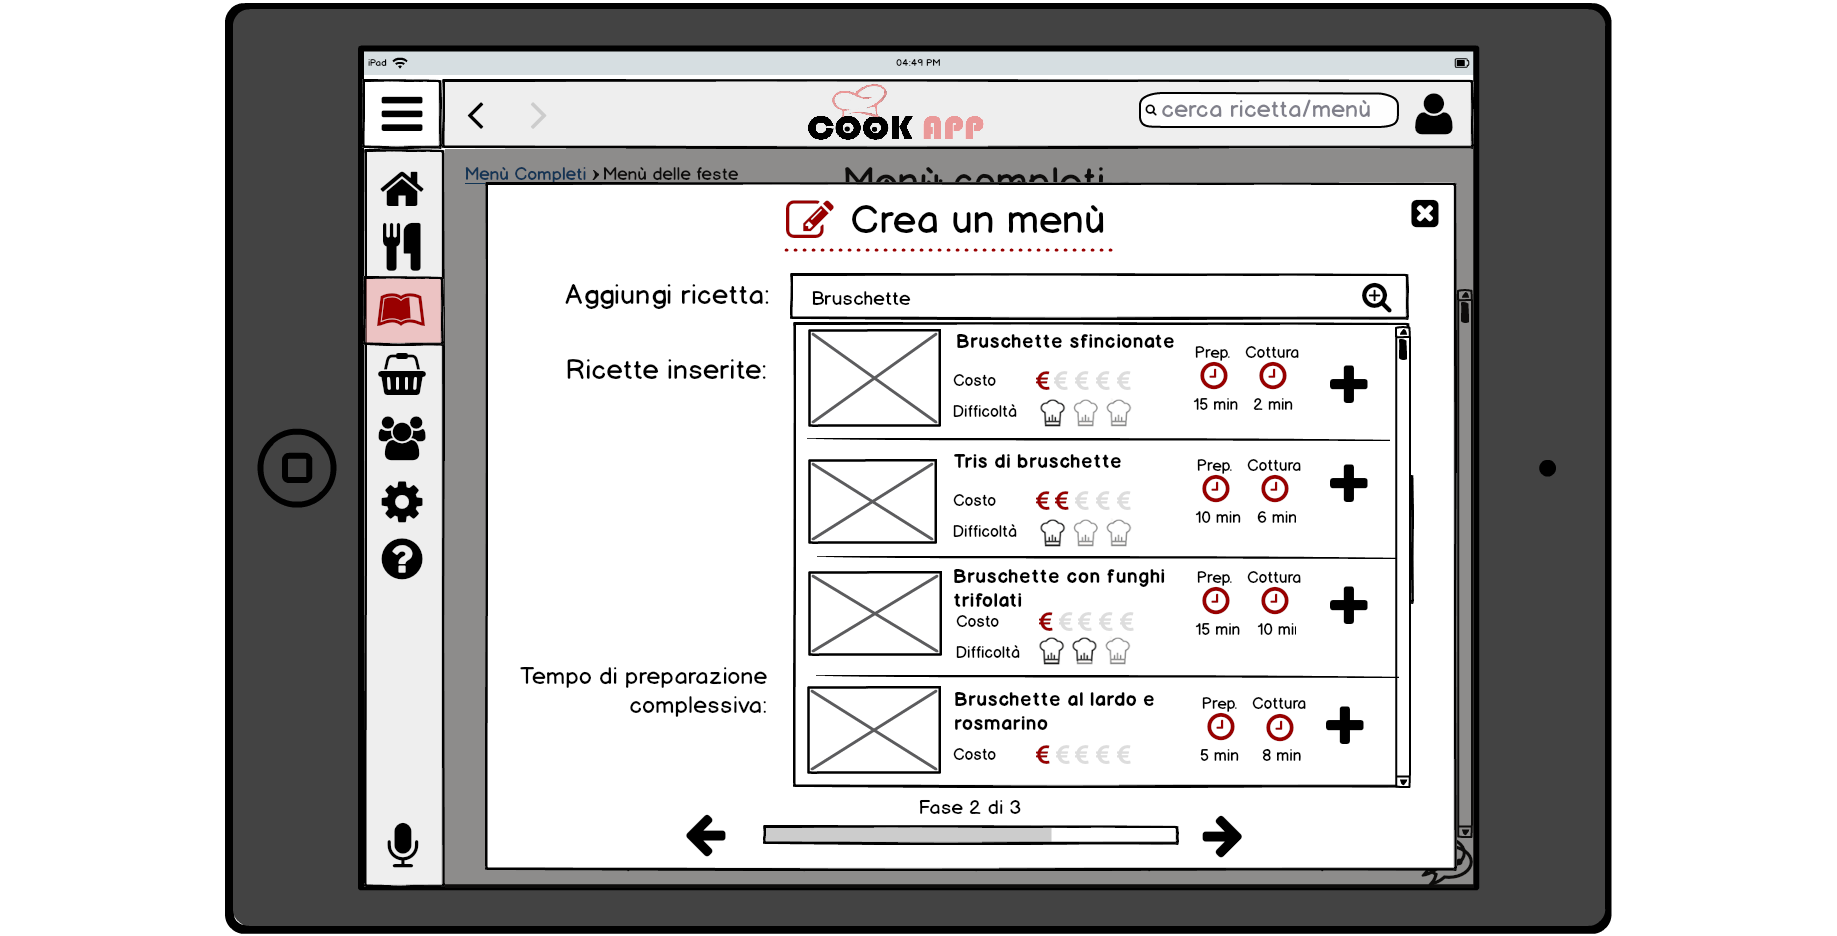
\includegraphics[width=0.95\linewidth]{img/mockup/menu-crea-3.png}
\end{figure}
\begin{figure}[H]
	\centering
	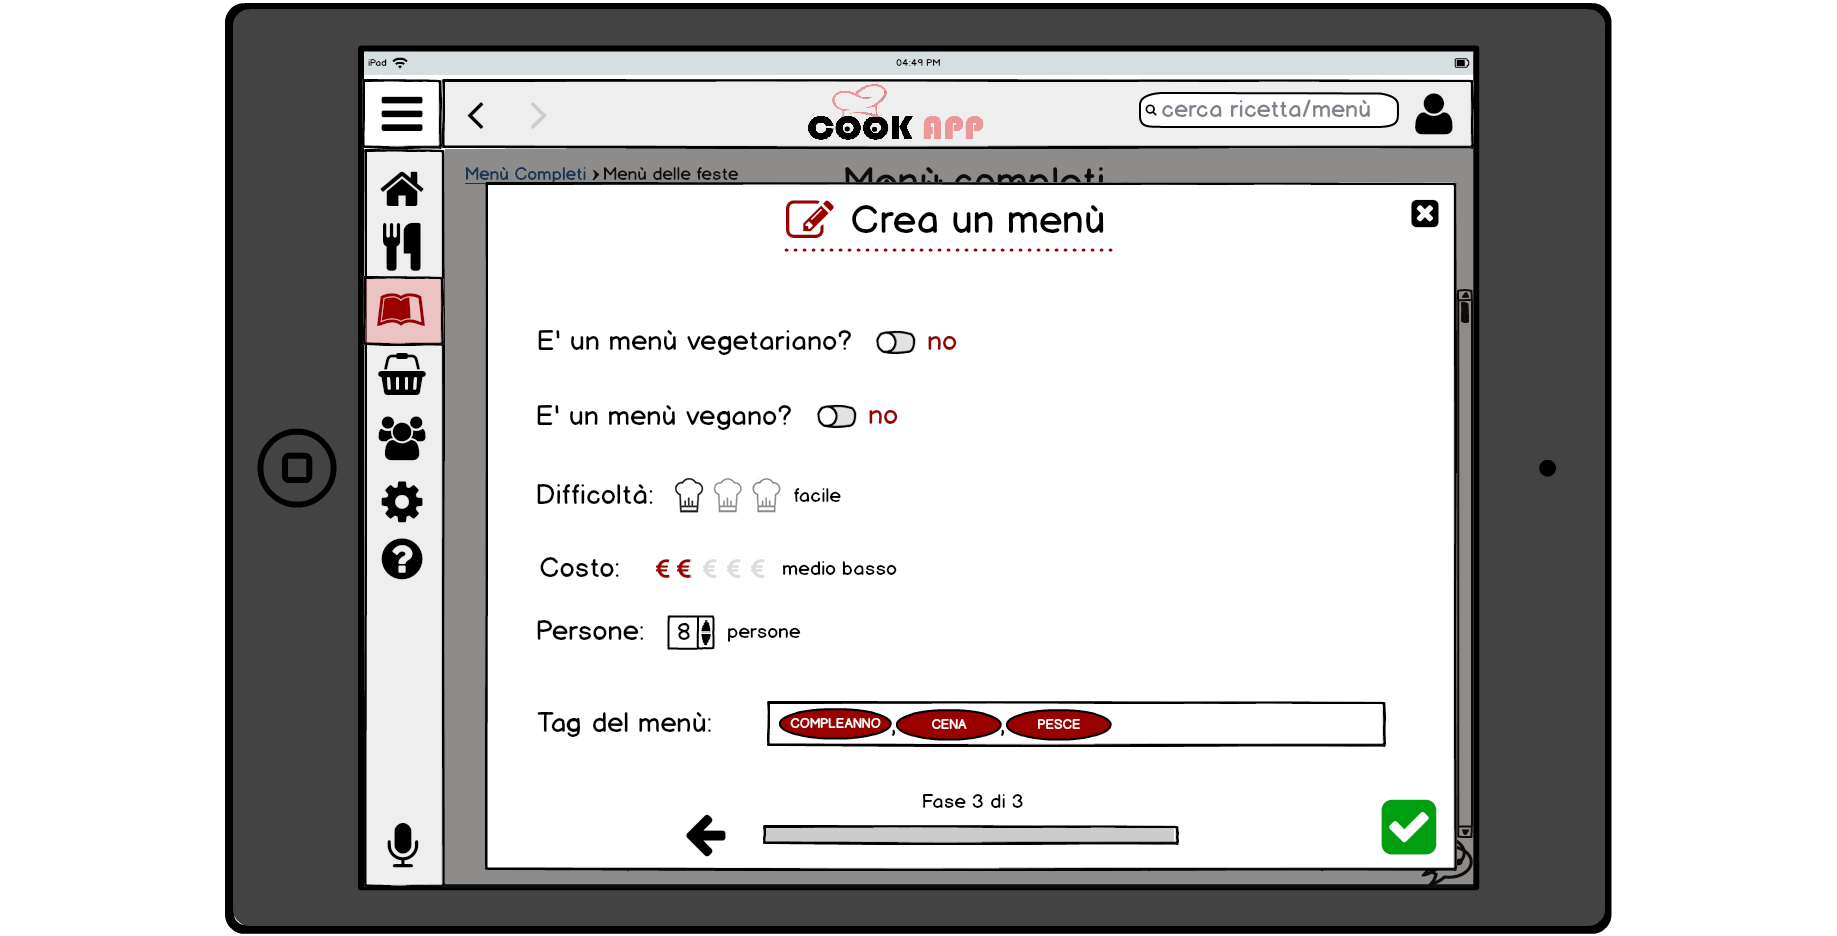
\includegraphics[width=0.95\linewidth]{img/mockup/menu-crea-4.png}
\end{figure}
\begin{figure}[H]
	\centering
	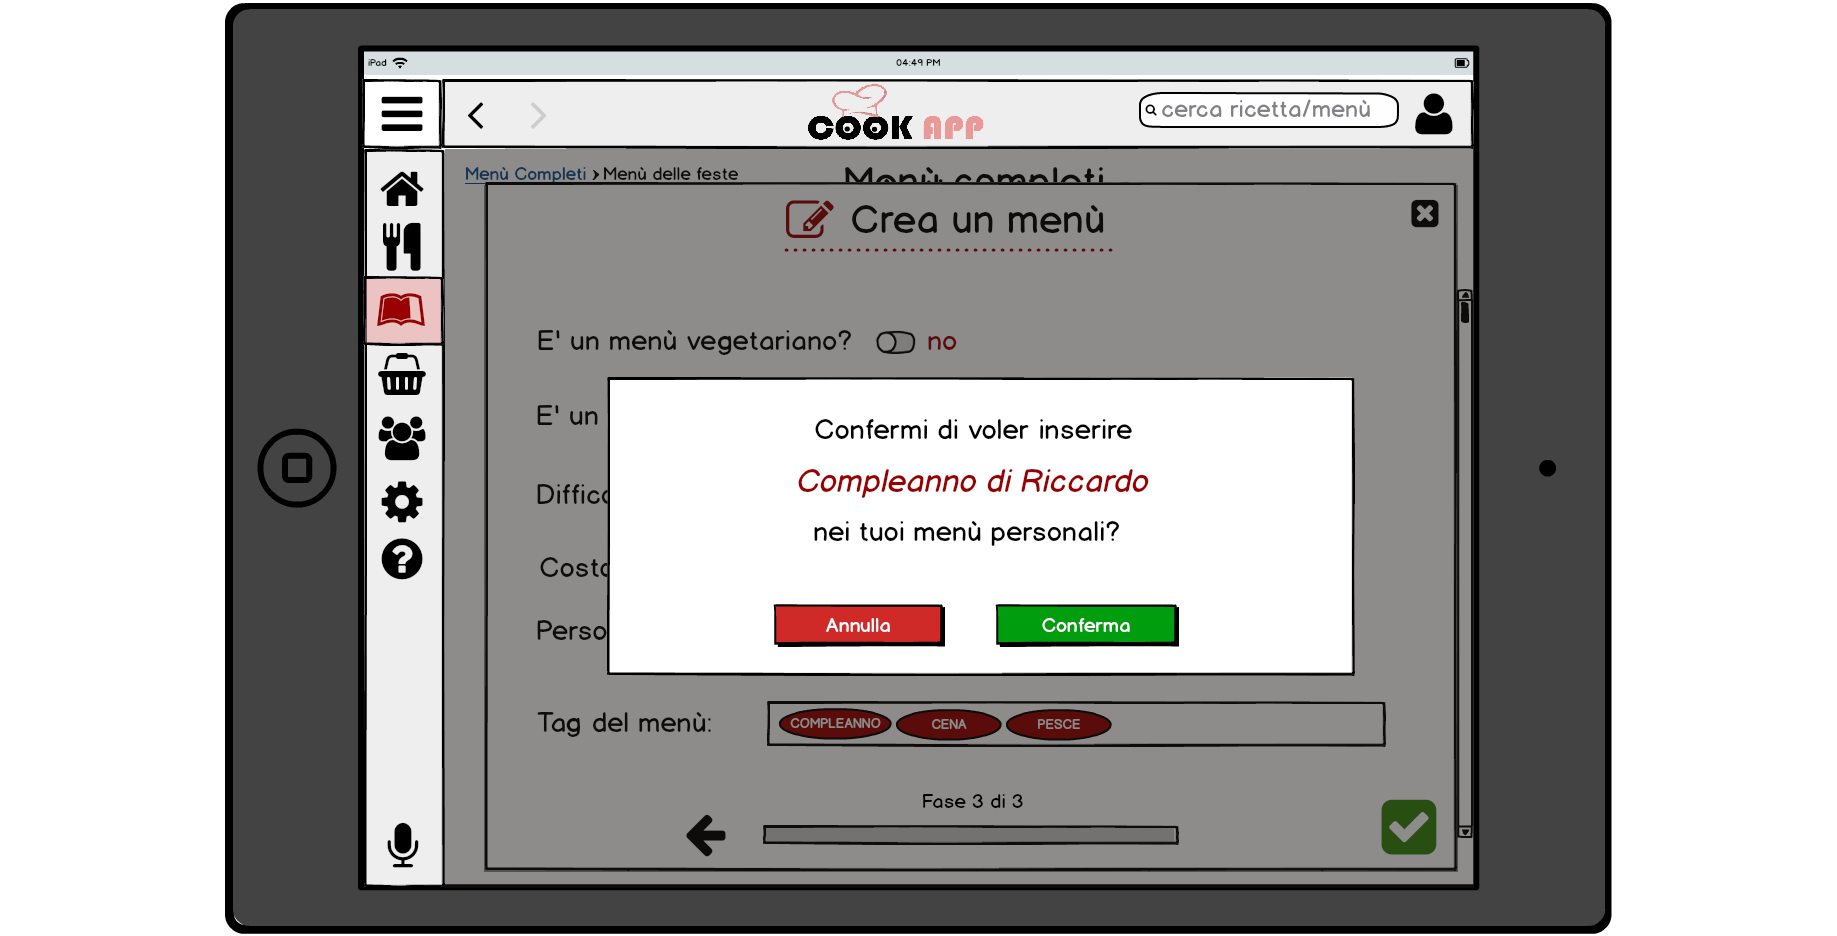
\includegraphics[width=0.95\linewidth]{img/mockup/menu-crea-5.png}
\end{figure}
\begin{figure}[H]
	\centering
	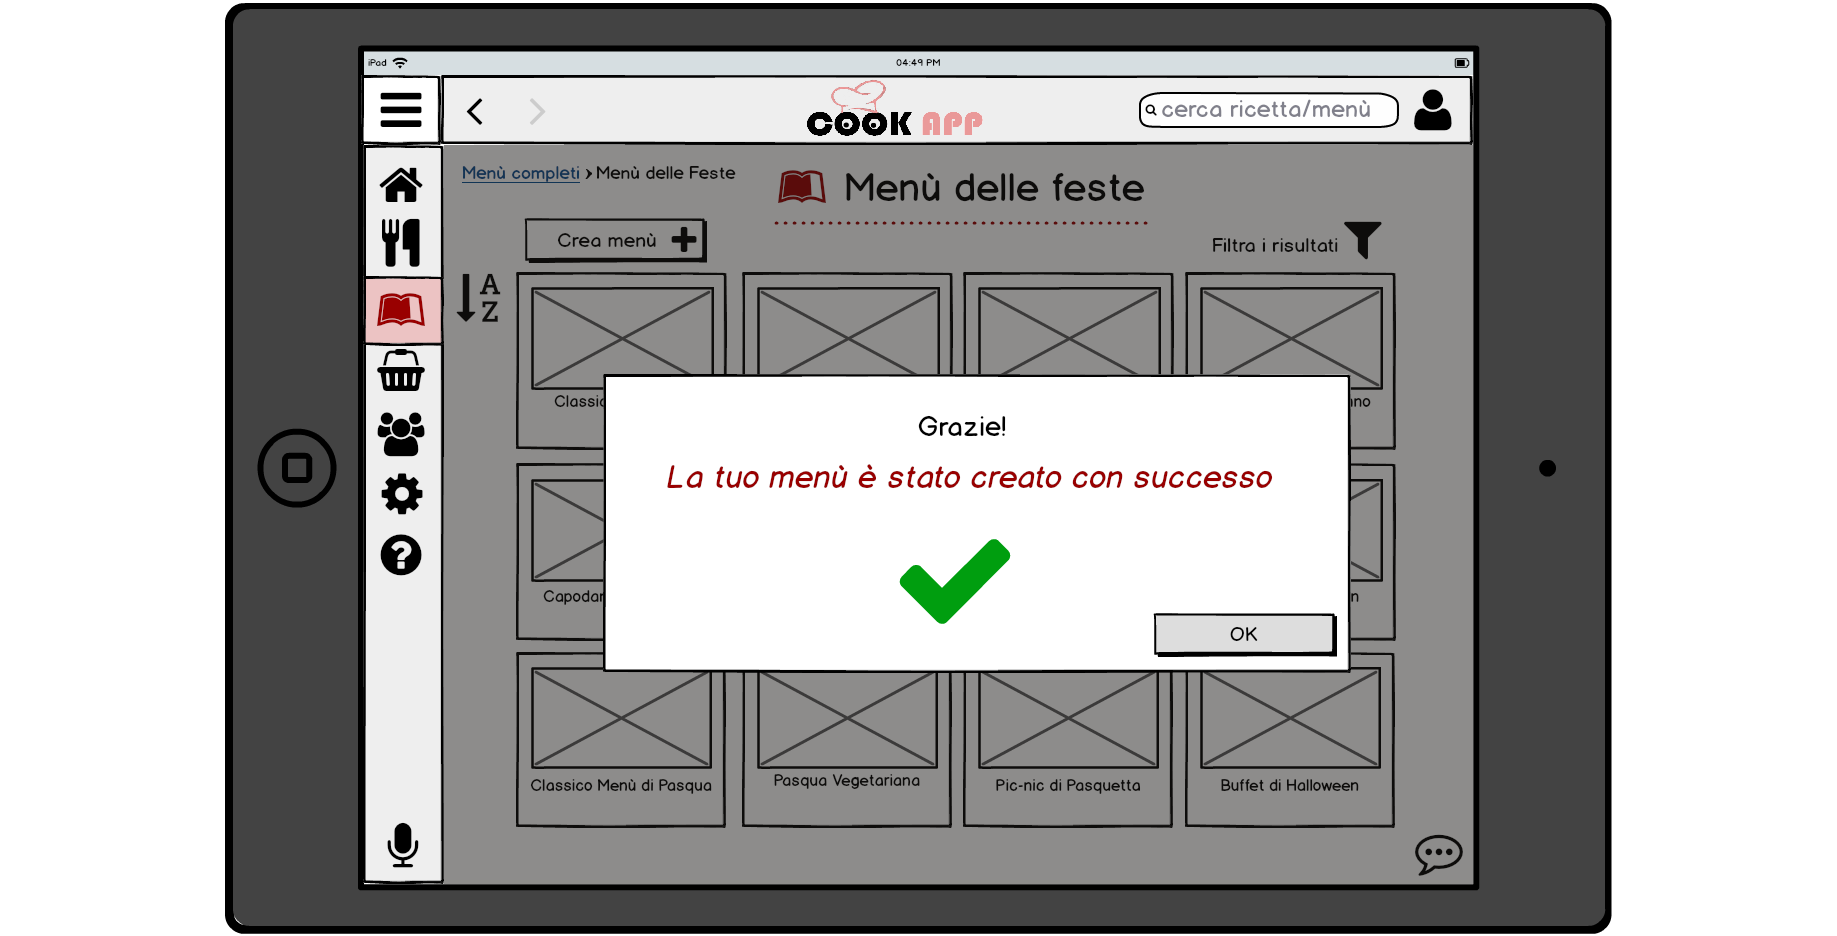
\includegraphics[width=0.95\linewidth]{img/mockup/menu-crea-6.png}
\end{figure}
\begin{figure}[H]
	\centering
	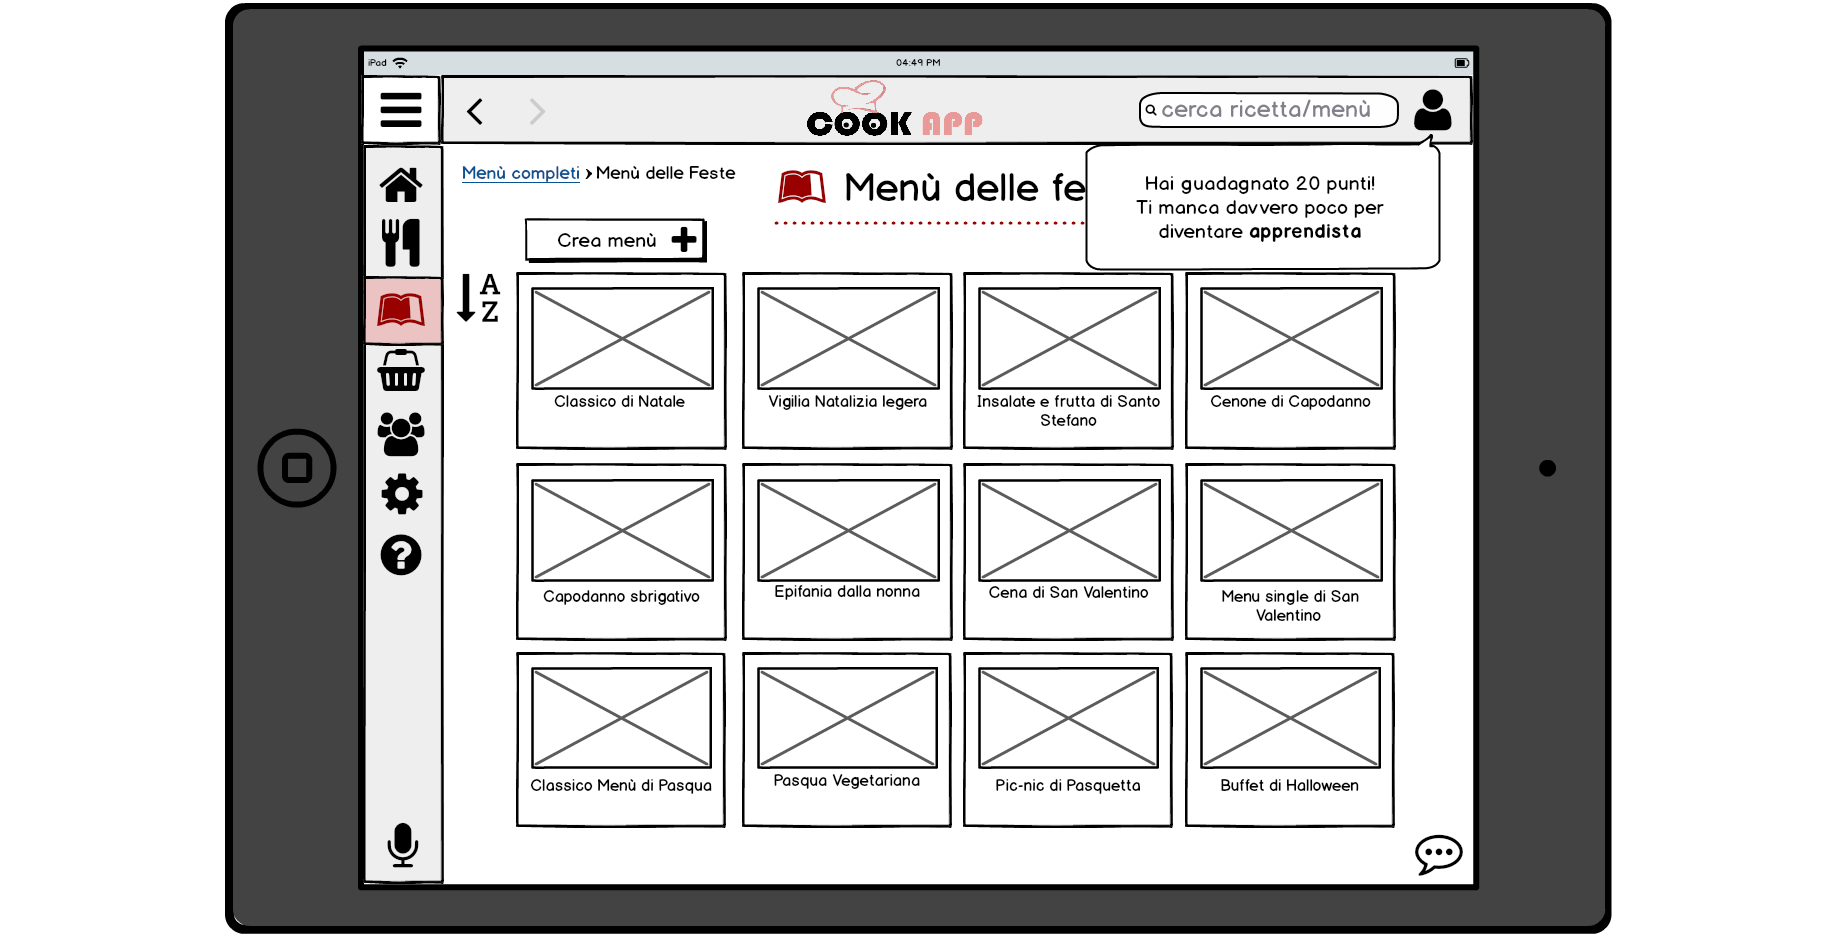
\includegraphics[width=0.95\linewidth]{img/mockup/menu-crea-7.png}
\end{figure}

\subsubsection{Lista della spesa}

TODO
\begin{figure}[H]
	\centering
	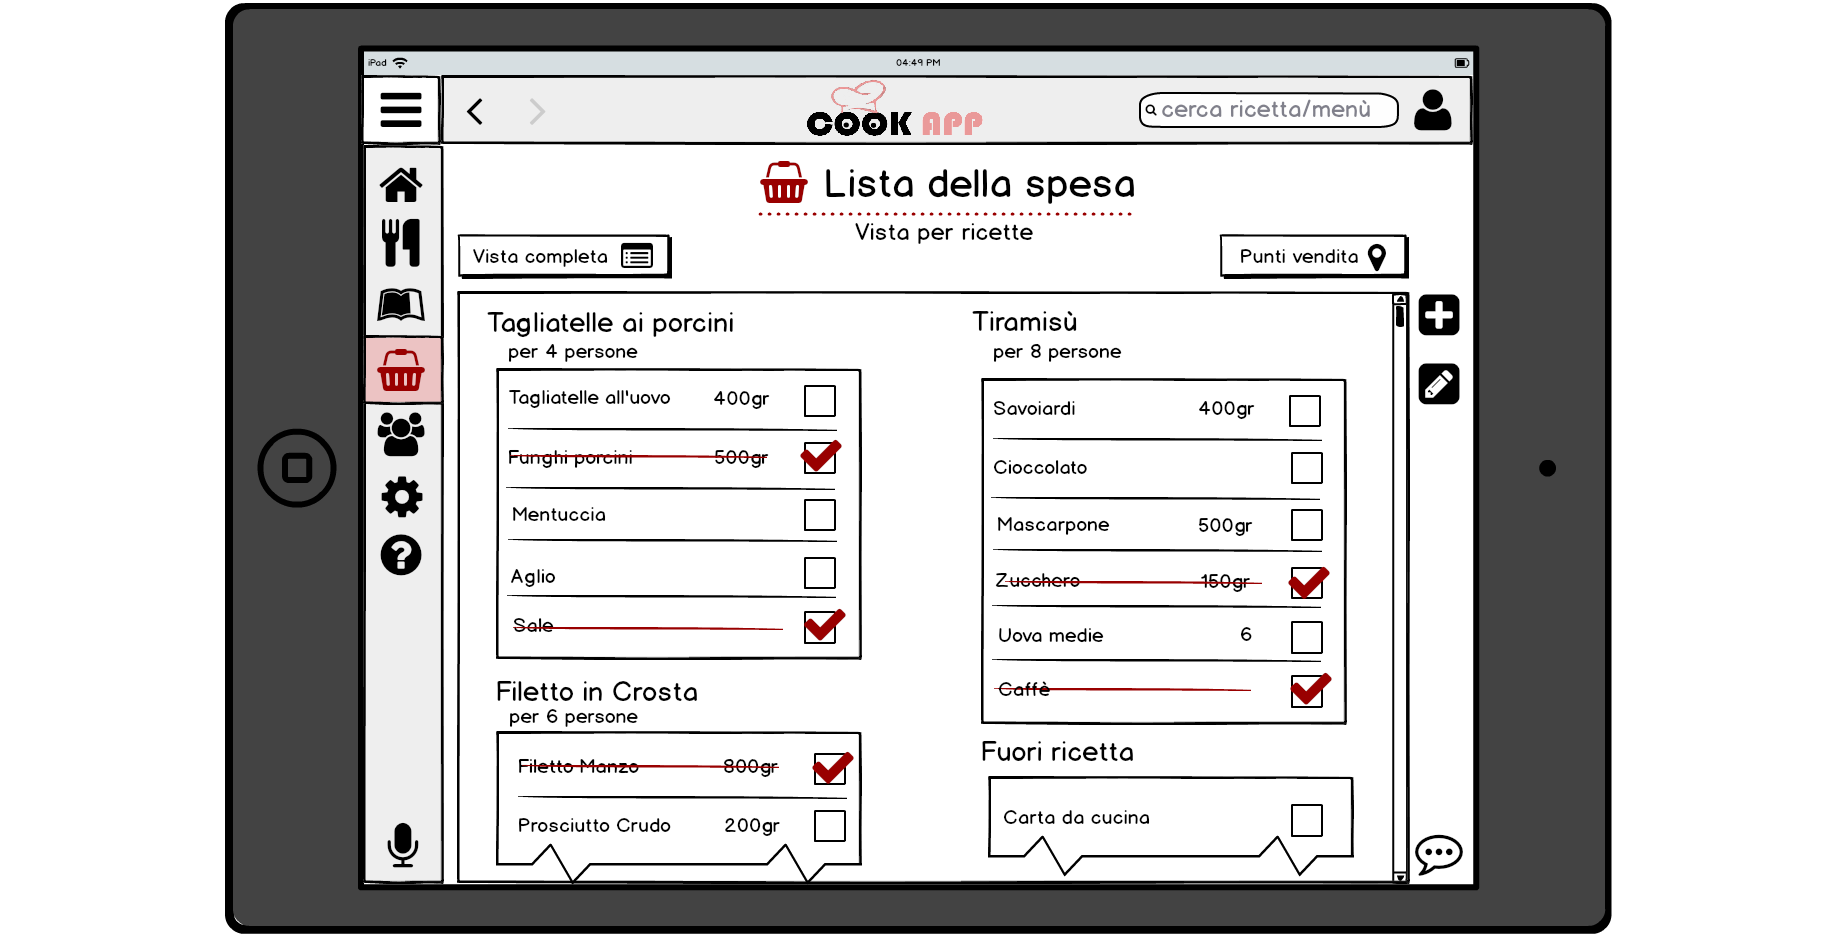
\includegraphics[width=0.95\linewidth]{img/mockup/spesa.png}
\end{figure}
\begin{figure}[H]
	\centering
	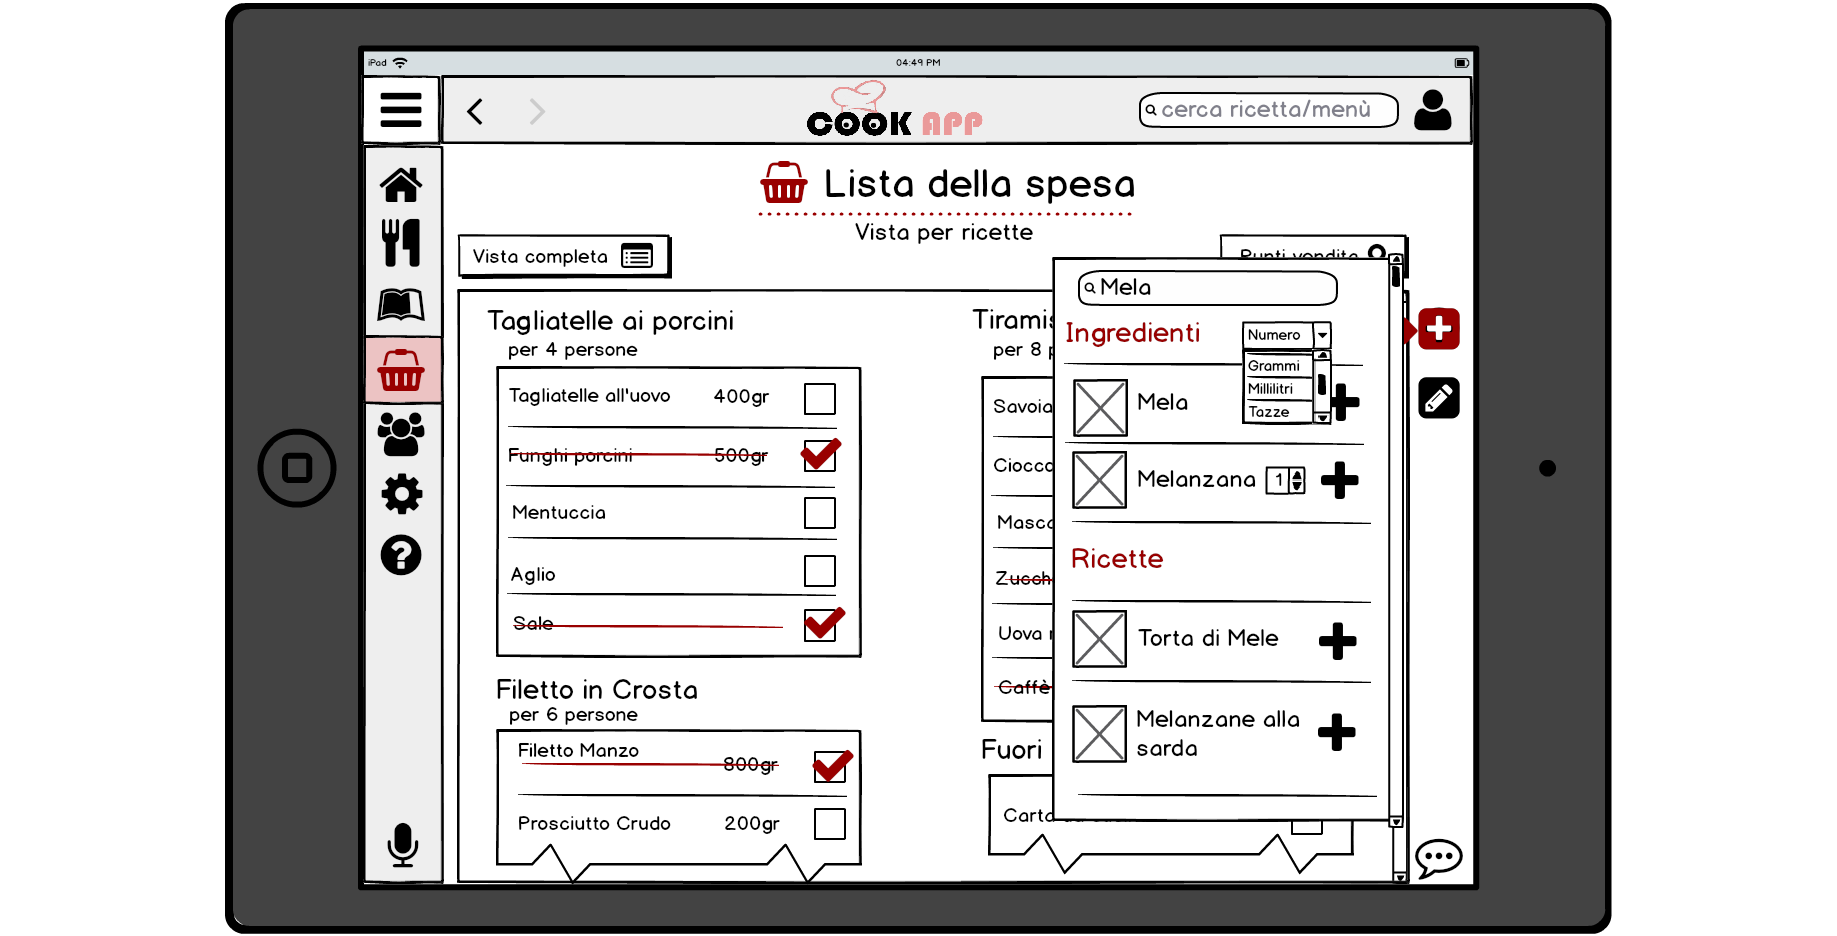
\includegraphics[width=0.95\linewidth]{img/mockup/spesa-add.png}
\end{figure}
\begin{figure}[H]
	\centering
	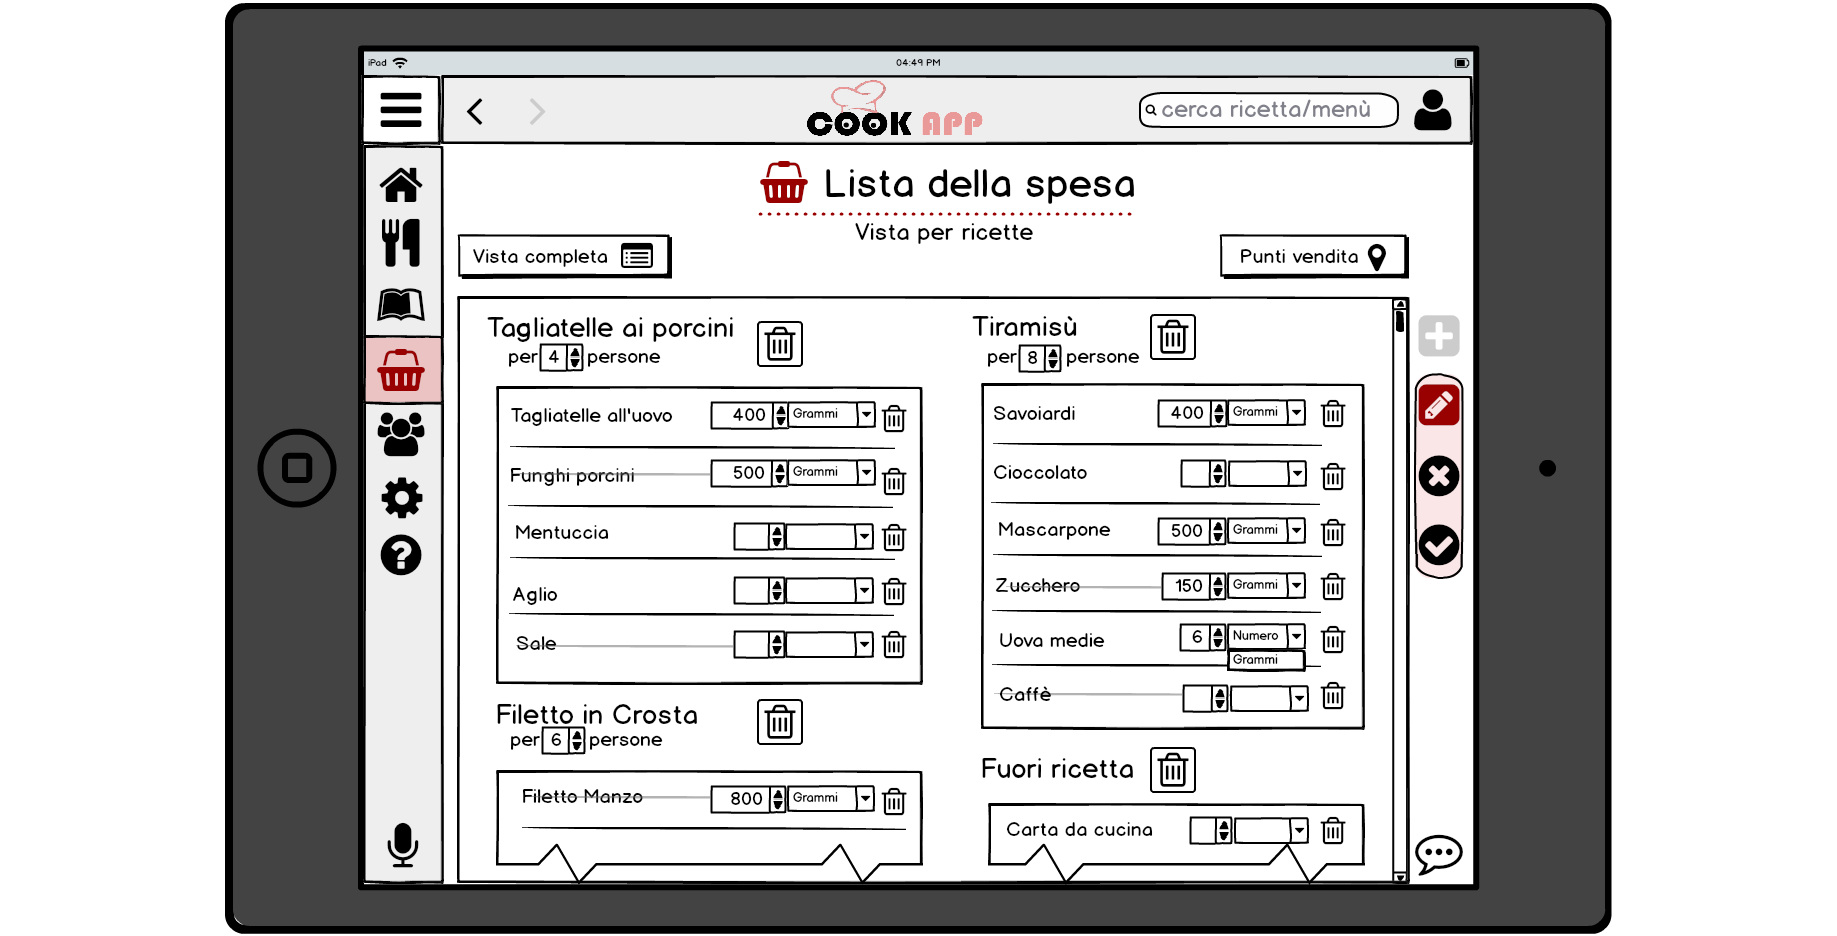
\includegraphics[width=0.95\linewidth]{img/mockup/spesa-edit.png}
\end{figure}
\begin{figure}[H]
	\centering
	\includegraphics[width=0.95\linewidth]{img/mockup/spesa-completa.png}
\end{figure}


\begin{figure}[H]
	\centering
	\includegraphics[width=0.95\linewidth]{img/mockup/punti-vendita.png}
\end{figure}
\begin{figure}[H]
	\centering
	\includegraphics[width=0.95\linewidth]{img/mockup/punti-vendita-2.png}
\end{figure}



\begin{figure}[H]
	\centering
	\includegraphics[width=0.95\linewidth]{img/mockup/zmart.png}
\end{figure}
\begin{figure}[H]
	\centering
	\includegraphics[width=0.95\linewidth]{img/mockup/zmart-vista-ricetta.png}
\end{figure}
\begin{figure}[H]
	\centering
	\includegraphics[width=0.95\linewidth]{img/mockup/zmart-add.png}
\end{figure}
\begin{figure}[H]
	\centering
	\includegraphics[width=0.95\linewidth]{img/mockup/zmart-punti-vendita.png}
\end{figure}





\subsubsection{Community}
TODO

\subsubsection{Profilo}
La sezione profilo mostra inizialmente alcune delle informazioni inserite nella fase di registrazione.\\
Nella sezione "Generale" è inizialmente mostrato un riepilogo delle azioni svolte di recente dall'utente o da altri utenti se questi hanno interagito con ricette/menù pubblicati. Sotto invece è possibile tenere d'occhio i progressi ottenuti nel sistema mediante un indicatore di punti esperienza e dei livelli sbloccati e sbloccabili.\\
Le sezioni "Le mie ricette" e "I miei menù", come suggerisce il nome indica ricette e menù pubblicati nel sistema con una rapida visione del numero di utenti che hanno inserito le ricette nei propri preferiti.\\
I propri preferiti sono archiviati nella sezione apposita: da qui è possibile rimuoverli, semplicemente trascinandoli verso il basso, verso la barra colorata con il simbolo del cestino.\\
Nel pannello di modifica del profilo è possibile modificare molti dei parametri inseriti durante la registrazione, insieme al livello di esperienza:
\begin{itemize}
\item L'utente novizio è quell'utente che non ha esperienza nè in ambito culinario nè in ambito tecnologico; il sistema è progettato per seguire passo-passo l'utente, offrendogli spesso messaggi di aiuto nelle operazioni svolte, come farebbe un amico fidato.
\item L'utente medio è l'utente che sa interagire bene col sistema, ma preferisce mantenere attive le funzionalità social per scambiare opinioni con la comunità ed eventualmente chiedere aiuto durante la preparazione della ricetta.
\item L'utente esperto non ha bisogno di funzionalità social che interferiscono con un uso metodico del sistema. 
\end{itemize}
\begin{figure}[H]
	\centering
	\includegraphics[width=0.95\linewidth]{img/mockup/Profilo-generale.png}
\end{figure}
\begin{figure}[H]
	\centering
	\includegraphics[width=0.95\linewidth]{img/mockup/Profilo-generale2.png}
\end{figure}
\begin{figure}[H]
	\centering
	\includegraphics[width=0.95\linewidth]{img/mockup/Profilo-menu.png}
\end{figure}
\begin{figure}[H]
	\centering
	\includegraphics[width=0.95\linewidth]{img/mockup/Profilo-modifica.png}
\end{figure}
\begin{figure}[H]
	\centering
	\includegraphics[width=0.95\linewidth]{img/mockup/Profilo-modifica2.png}
\end{figure}
\begin{figure}[H]
	\centering
	\includegraphics[width=0.95\linewidth]{img/mockup/Profilo-preferiti.png}
\end{figure}
y\begin{figure}[H]
	\centering
	\includegraphics[width=0.95\linewidth]{img/mockup/Profilo-preferiti2.png}
\end{figure}
\begin{figure}[H]
	\centering
	\includegraphics[width=0.95\linewidth]{img/mockup/Profilo-ricette.png}
\end{figure}
\subsubsection{Impostazioni}
Qui vi sono le principali impostazioni previste dall'applicazione.\\ Normalmente questa imposterà di default la lingua del sistema, ma se si vuole è possibile cambiarla da un apposito menù a tendina.\\
Le difficoltà della lettura possono essere risolte aumentando qui la grande del font.\\
Se i suoni dell'applicazione o delle notifiche provoca disturbo, qui è possibile disattivarle.\\
Infine è possibile definire qual è la visualizzazione preferita dei procedimenti delle ricette, insieme al sistema di misura utilizzato per pesare gli ingredienti.\\
\begin{figure}[H]
	\centering
	\includegraphics[width=0.95\linewidth]{img/mockup/Impostazioni.png}
\end{figure}
\subsubsection{Help}
In questa sezione l'utente troverà, in ogni momento, la possibilità di leggere in modo dettagliato ogni funzionalità dell'applicazione, insieme alle risposte delle domande più frequenti (FAQ).
\begin{figure}[H]
	\centering
	\includegraphics[width=0.95\linewidth]{img/mockup/Help.png}
\end{figure}
